\documentclass[12pt]{article}

\usepackage{fullpage}
\usepackage{graphicx, rotating, booktabs} 
\usepackage{times} 
\usepackage{natbib} 
\usepackage{indentfirst} 
\usepackage{setspace}
\usepackage{grffile} 
\usepackage{hyperref}
\usepackage{adjustbox}
\usepackage{amsmath}
\usepackage{siunitx}
\usepackage{multirow}
\setcitestyle{aysep{}}


\singlespace
\title{\textbf{Appendix: Elite Cues and Public Attitudes Towards Military Alliances}}
\author{}
\date{}

\bibliographystyle{apsr}

\begin{document}

\maketitle 

\doublespace 


In this appendix, I provide further background on the results in the manuscript. 
I start by presenting the conjoint attributes, followed by inferences about alliance characteristics. 
After that, I divide responses to elite cues and alliance characteristics based on foreign policy dispositions and partisanship alone. 
I then analyze responses to an open ended question, and compare results with the rating and choice measures.
Last, I present some descriptive data on key demographics and the experimental treatments. 


\tableofcontents

\newpage

\section{Noteworthy Alliance Characteristics}

Some alliance characteristics influence alliance attitudes as well, as \autoref{fig:joint-plot} shows. 
Allied regime type is particularly consequential. 
Established democracy increases support for alliance formation and maintenance.
The magnitude of the established democracy AMCE is comparable to elite cues.   
Weak democracies are marginally more likely than non-democracies to receive public support for an alliance.


\begin{figure}[htpb]
	\centering
		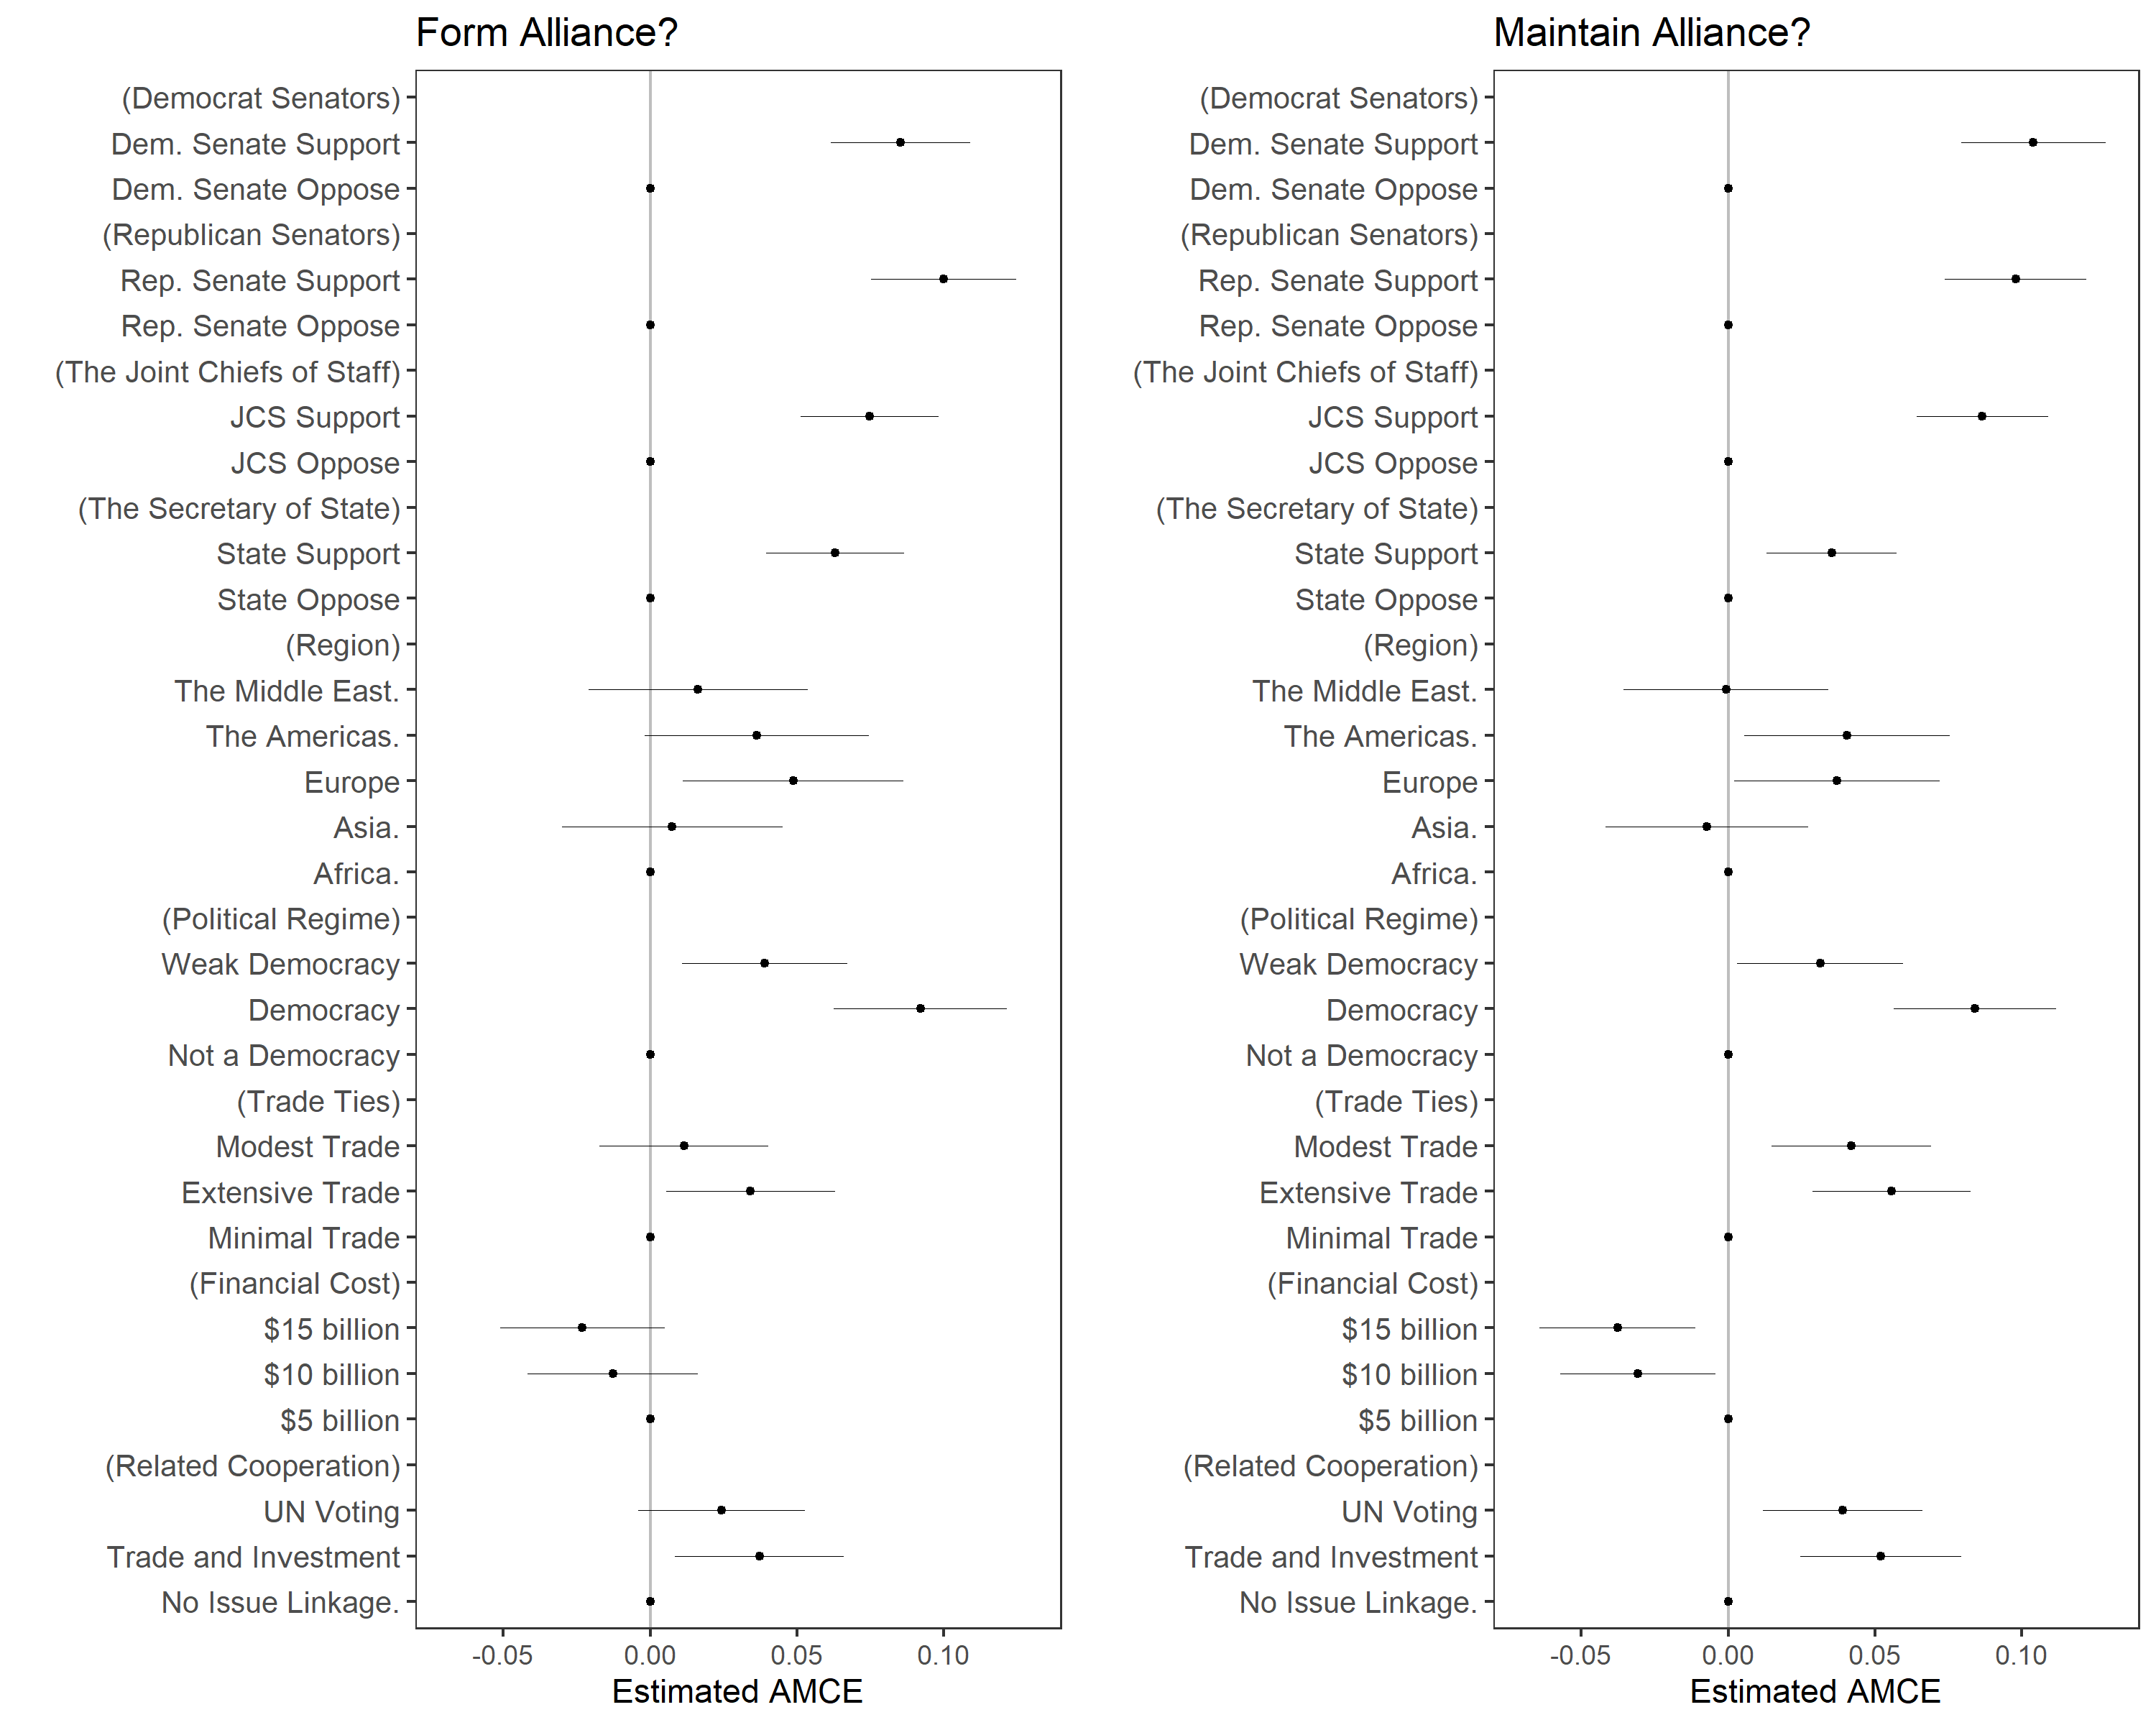
\includegraphics[width=0.95\textwidth]{joint-amce-plots.png}
	\caption{Average marginal component effect of elite cues and alliance characteristics on public support for forming or maintaining a hypothetical military alliance. Feature names in parentheses. Estimates with a dot at zero are the base attribute level. Components marked with abbreviated labels and some attributes omitted to make the plot more legible.}
	\label{fig:joint-plot}
\end{figure}



Issue linkages also encourage support for alliance formation and maintenance. 
Linkages to trade and investment with the United States increase support for alliance participation, relative to an alliance with no linkages. 
Political issue linkages in the United Nations bolster individual support, though this effect is smaller than that of trade. 
This result adds a public opinion mechanism to prior claims that issue linkages can facilitate new alliance agreements \citep{Poast2012} and bolster alliance credibility \citep{Poast2013}. 


Last, alliance context and costs shift public attitudes. 
Trade ties and serious common threat encourage support for alliance maintenance. 
Relative to the lowest annual military spending cost, annual costs of \$10 billion or more decrease support for upholding an alliance.  
Respondents also view alliances in Europe or the Americas more favorably than commitments in Africa. 

%\section{Alliance Characteristics, Partisanship and Foreign Policy Dispositions}


% partisan differences in democracy
As with elite cues, foreign policy dispositions and partisanship mold individual responses to alliance characteristics. 
\autoref{fig:party-dispo-form-char} and \autoref{fig:party-dispo-main-char} summarize partisan and dispositional differences in alliance characteristics treatments from the formation and maintenance experiments. 
Both figures present the marginal mean of alliance support for Republicans and Democrats with different foreign policy dispositions under key alliance characteristics treatments, as well as lines summarizing the overall mean choice in each group. 


Allied democracy is an area of bipartisan agreement among individuals with different foreign policy dispositions.
When allied democracy changes in the alliance formation experiment, Republicans and Democrats with identical foreign policy dispositions shift their attitudes in similar ways. 
Internationalists in both major parties value allied democracy. 


Democrats express strong support for democratic alliance partners in the maintenance experiment. 
Dovish Democrats are skeptical of alliances with non-democracies, relative to other treaties. 
Republicans hold more mixed views of allied political regimes. 
While internationalist Republicans hold similar views to Democrats, isolationist Republicans place less weight on allied democracy, especially in alliance maintenance. 


\begin{figure}[htpb]
	\centering
		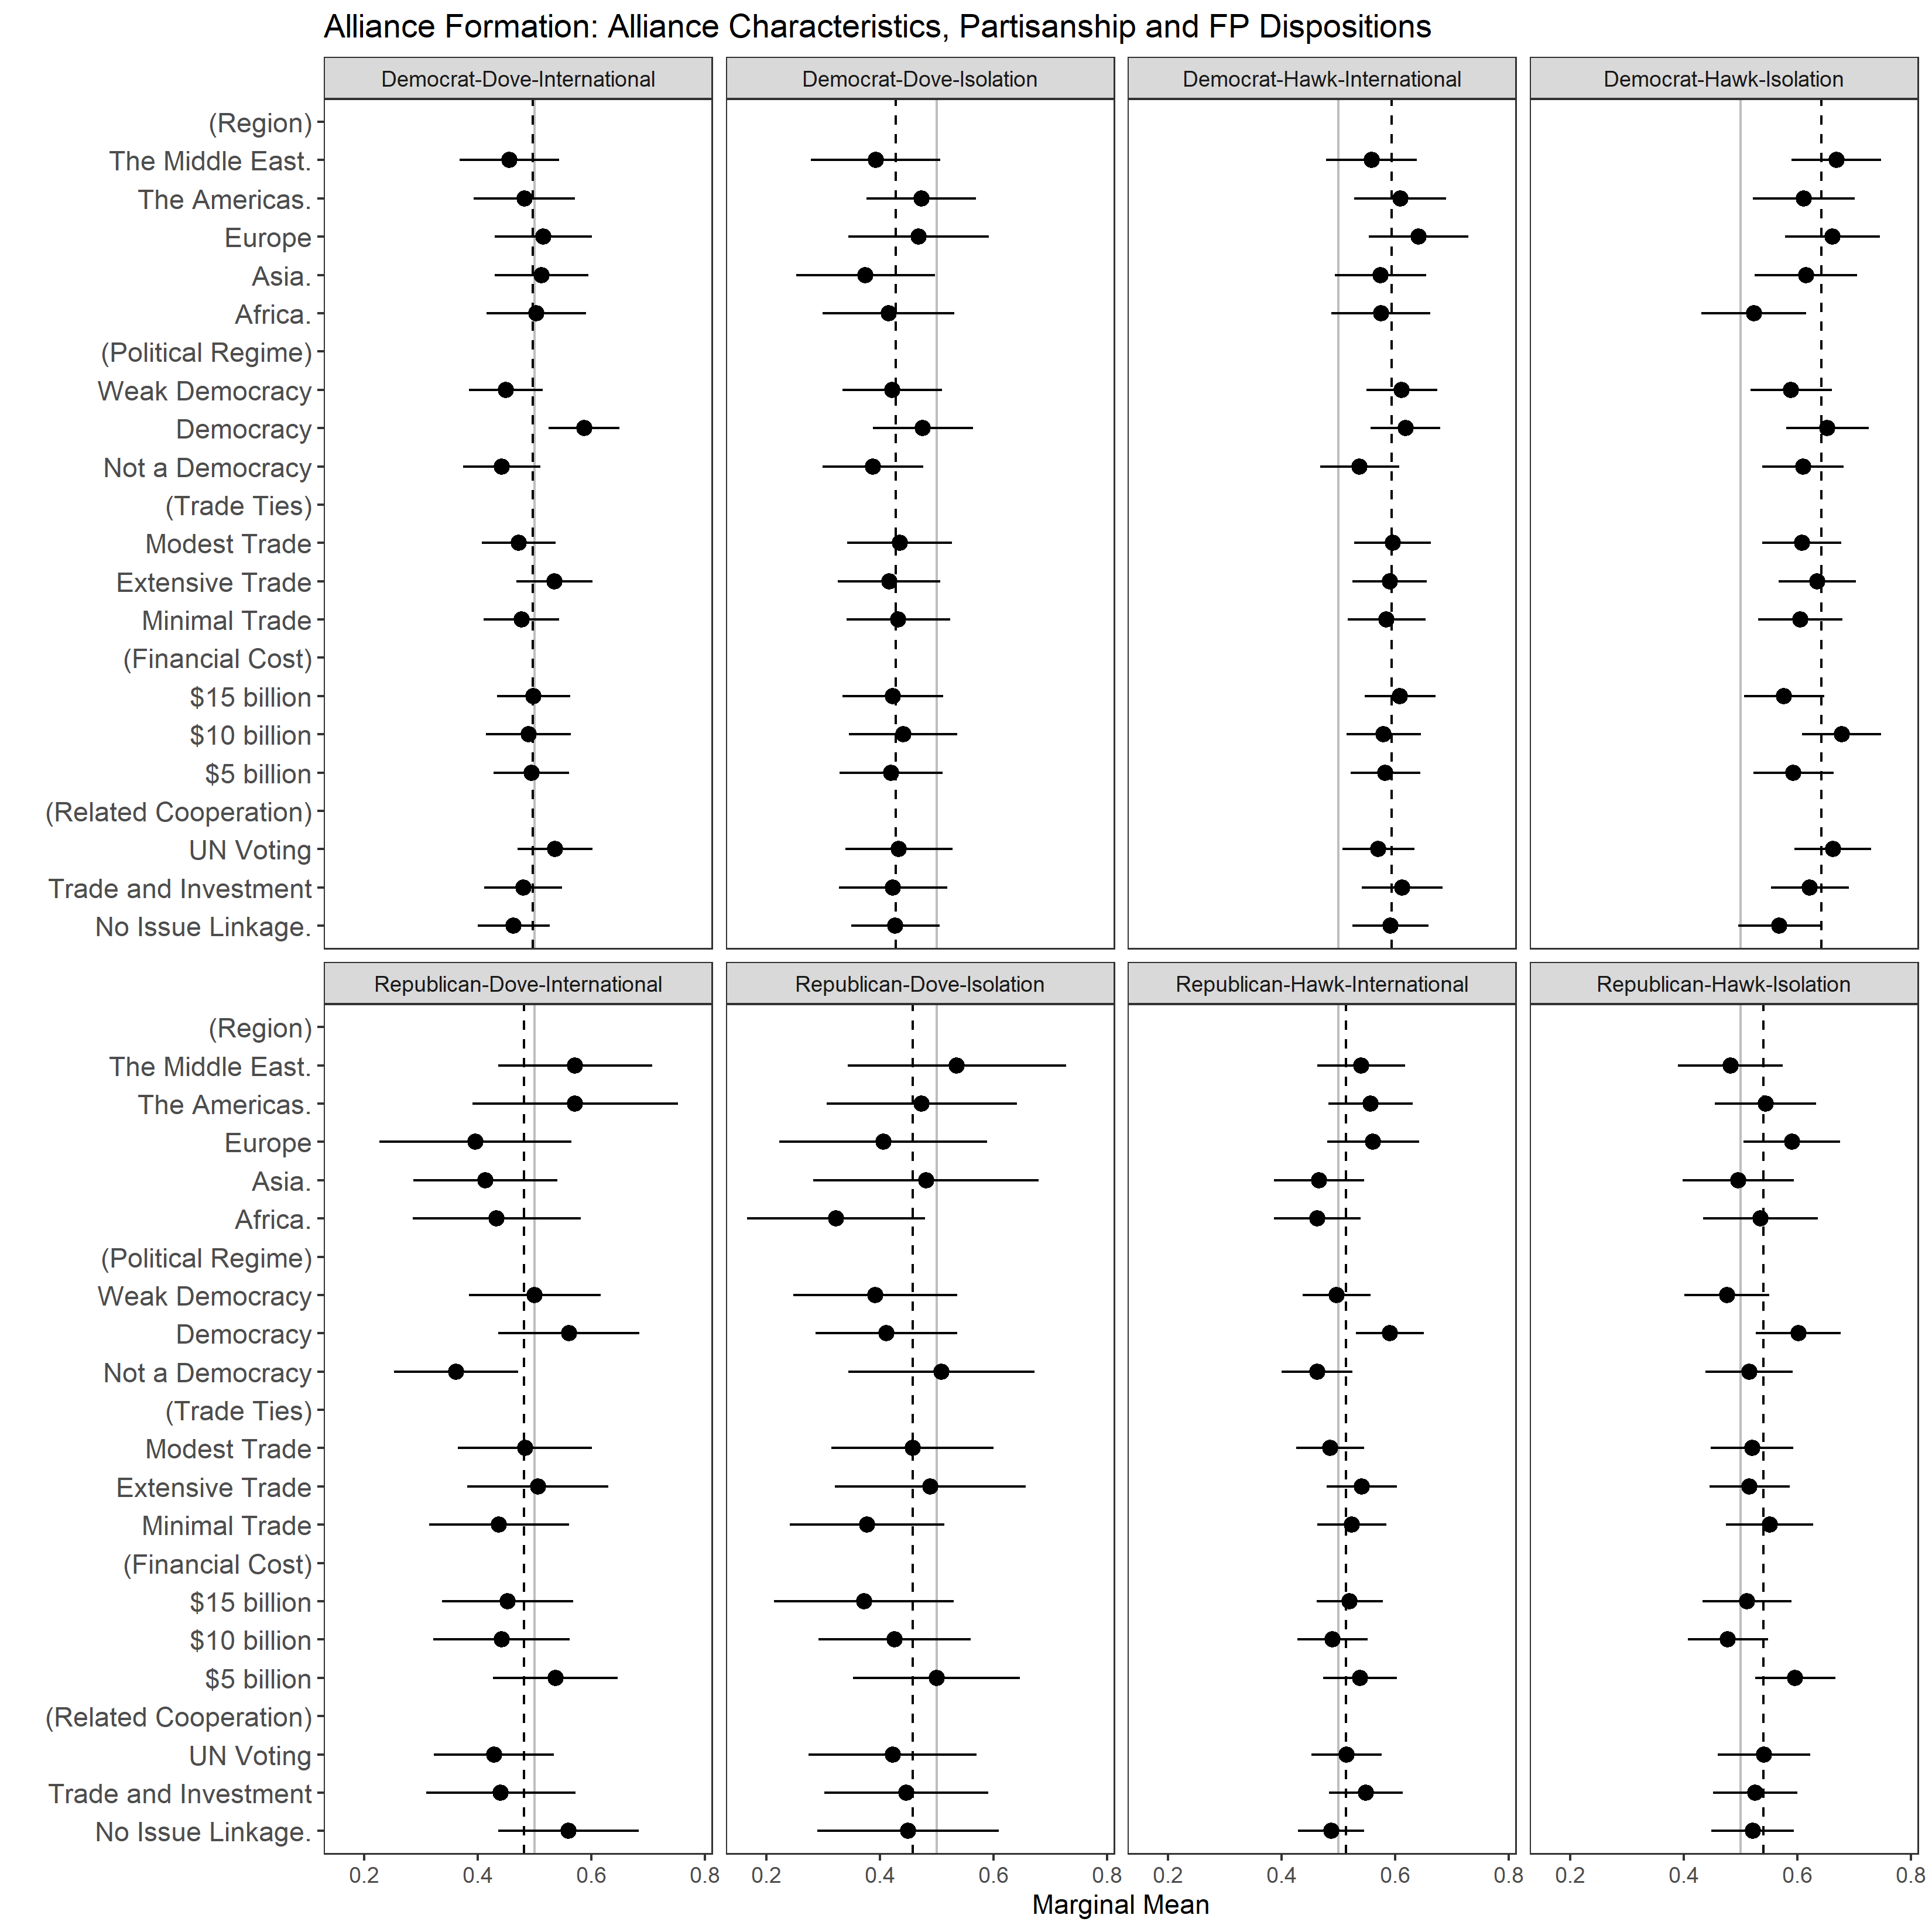
\includegraphics[width=0.95\textwidth]{party-dispo-form-char.png}
	\caption{Marginal means of support for forming hypothetical alliances across party identification and foreign policy dispositions given different key alliance characteristics. For each group, the estimates mark the marginal mean of support for alliance participation under different alliance treatments. The solid vertical line marks a marginal mean of .5, while the dashed line marks the average choice across all levels. Components marked with abbreviated labels and some attributes omitted to make the plot more legible. Independents omitted.}
	\label{fig:party-dispo-form-char}
\end{figure}



\begin{figure}[htpb]
	\centering
		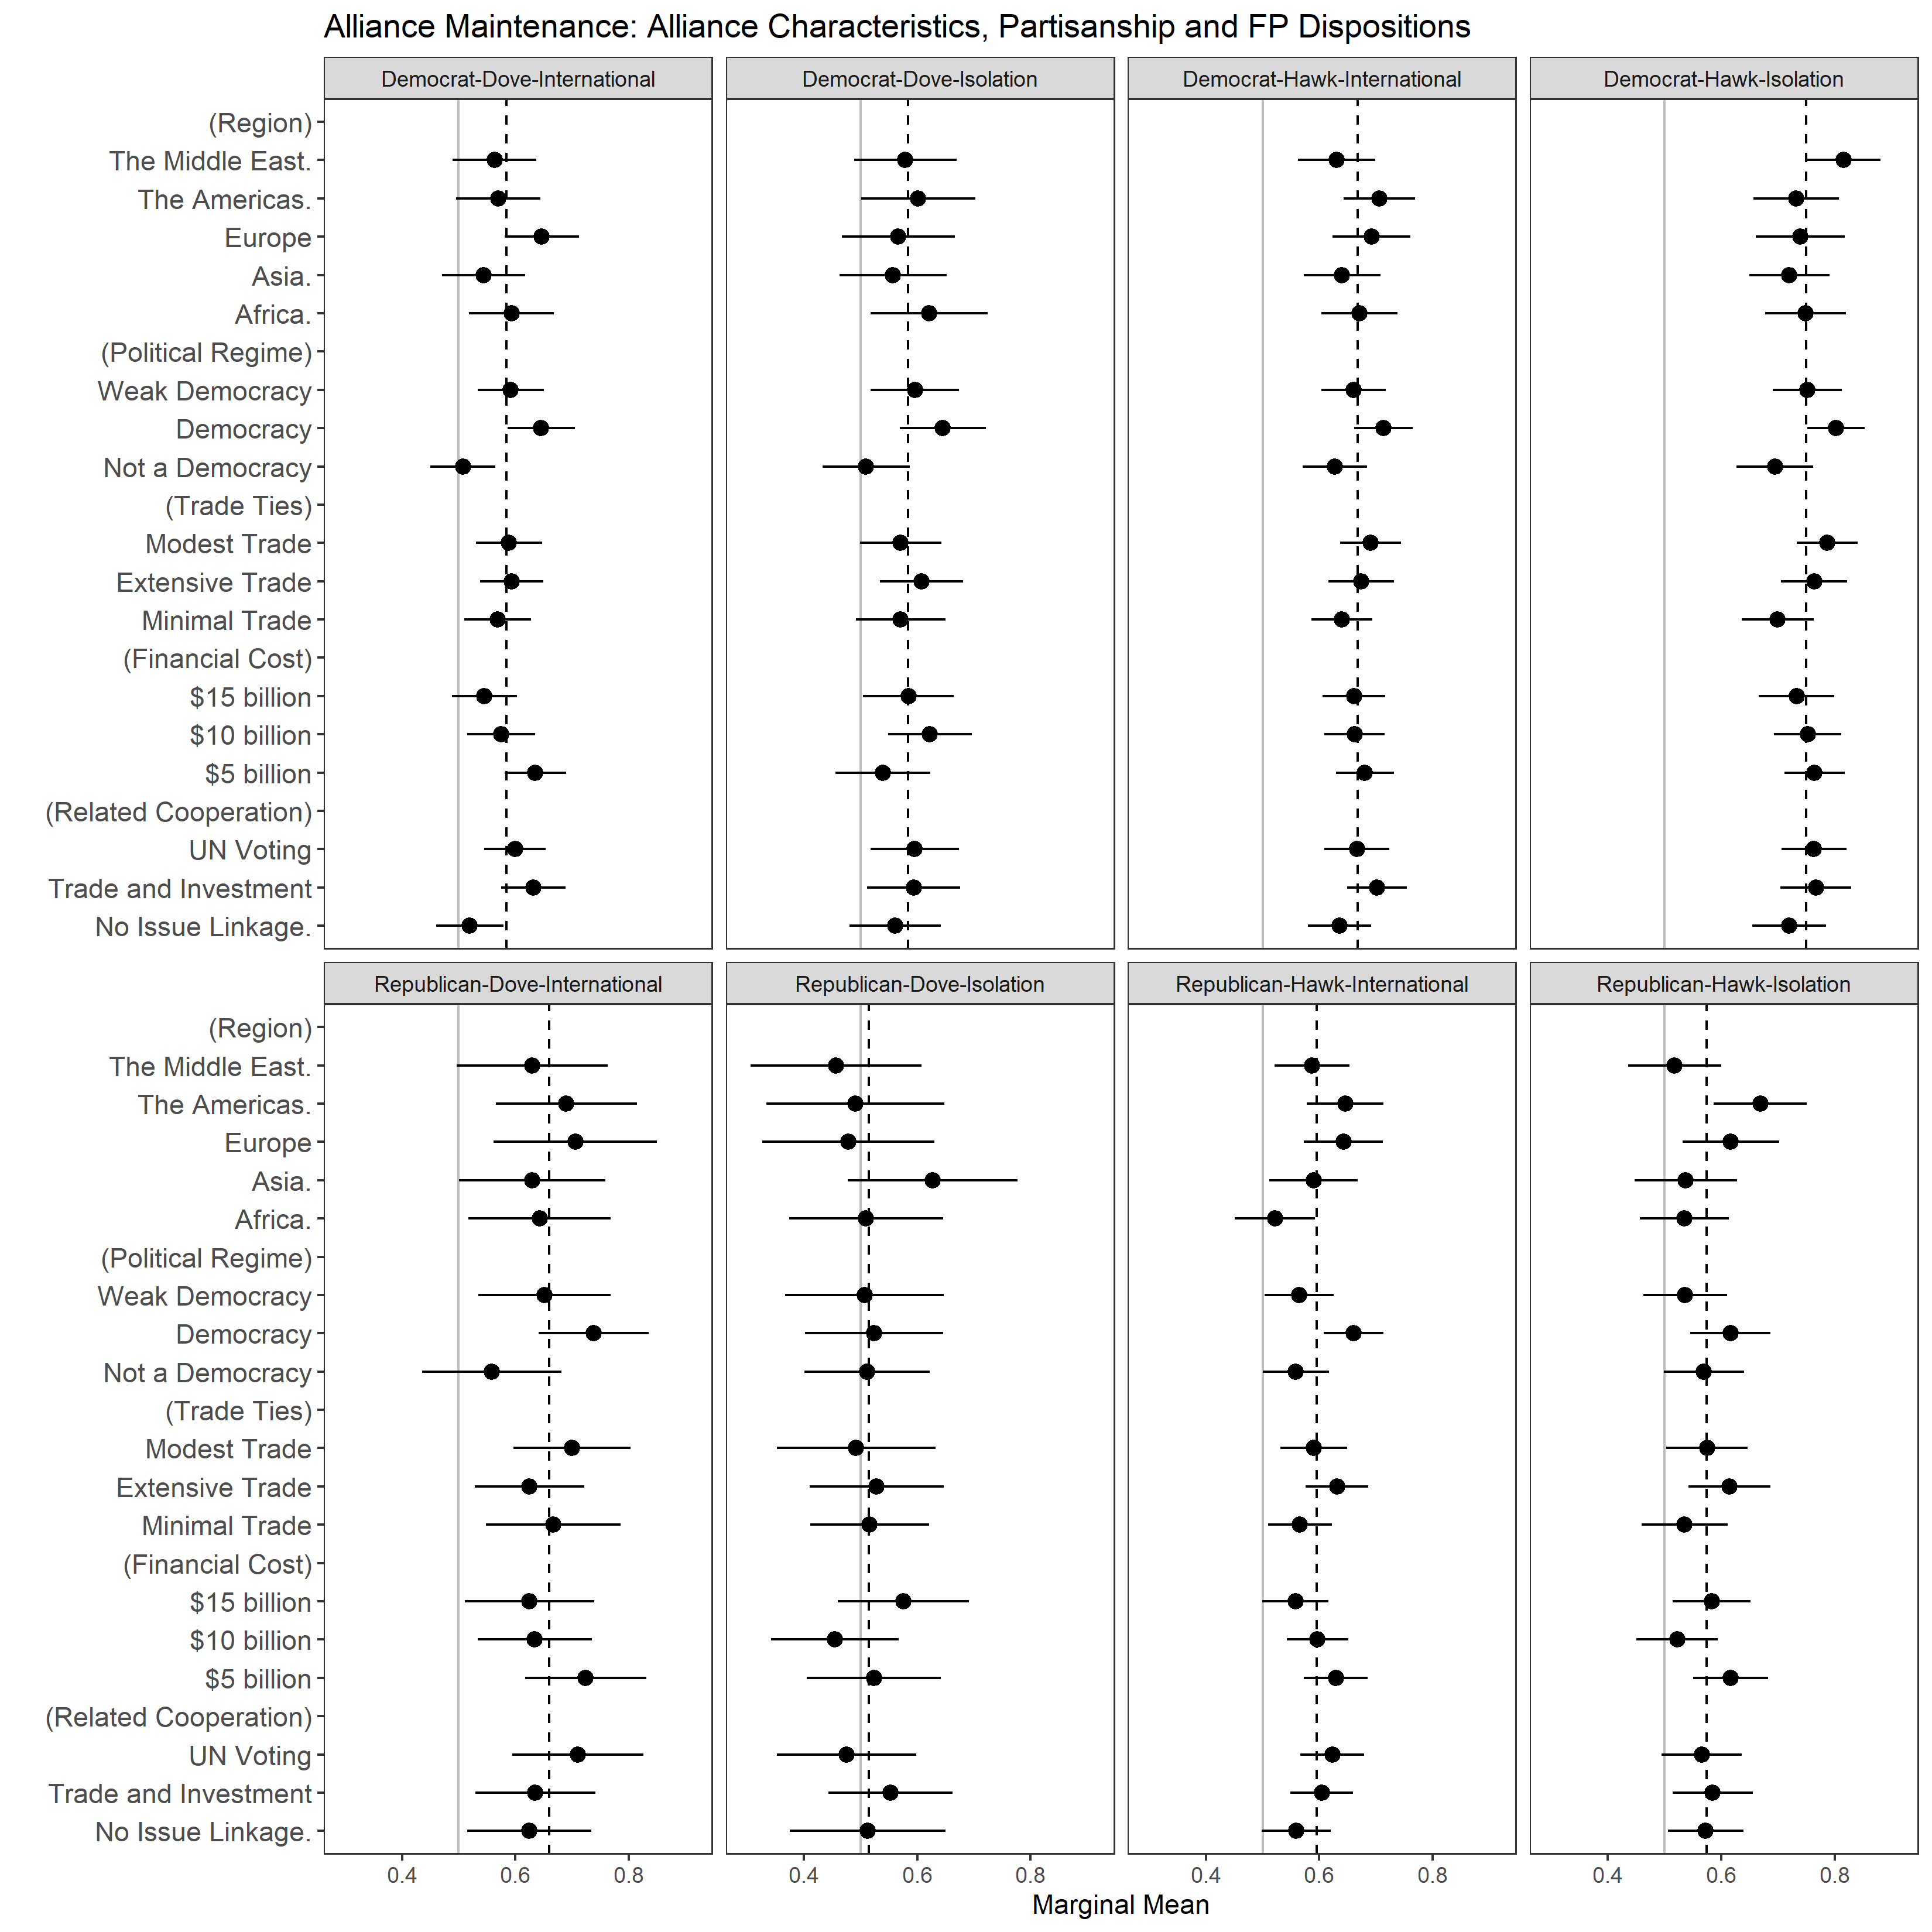
\includegraphics[width=0.95\textwidth]{party-dispo-main-char.png}
	\caption{Marginal means of support for maintaining hypothetical alliances across party identification and foreign policy dispositions given different key alliance characteristics. For each group, the estimates mark the marginal mean of support for alliance participation under different alliance treatments. The solid vertical line marks a marginal mean of .5, while the dashed line marks the average choice across all levels. Components marked with abbreviated labels and some attributes omitted to make the plot more legible. Independents omitted.}
	\label{fig:party-dispo-main-char}
\end{figure}


% Some points of consistency
Support for international engagement also produces some partisan overlap. 
Internationalists are more responsive to trade and foreign policy issue linkages than isolationists. 
In the alliance maintenance experiment, dovish and internationalist individuals are more likely to reduce their support as alliance costs increase.


% other differences in region
%Both experiments uncover partisan differences in attitudes towards alliances in different regions. 
%Hawkish Republicans oppose alliances with African countries and prefer alliances in Europe or the Americans. 
%Democrats with similar foreign policy dispositions express no regional preferences.  


\newpage


\section{Alliance Support by Foreign Policy Disposition} 


The manuscript reports analyses that divide respondents by partisanship and foreign policy disposition. 
In this section of the appendix, I report subgroup analyses by foreign policy disposition alone, which are also consistent with the manuscript results.
\autoref{fig:hawk-plots} and \autoref{fig:isolation-plots} plot the marginal means of elite cues and alliance characteristics across militant assertiveness and isolationism. 


Hawkish individuals are more likely to support alliance formation and maintenance, regardless of the experimental treatments. 
Hawks also respond to cues from Republican Senators and the Joint Chiefs of Staff. 
Doves pay more attention to cues from Democratic Senators.
These differences are evident in the manuscript results, as Republicans are more hawkish, and Democrats more internationalist on average. 


\begin{figure}
	\centering
		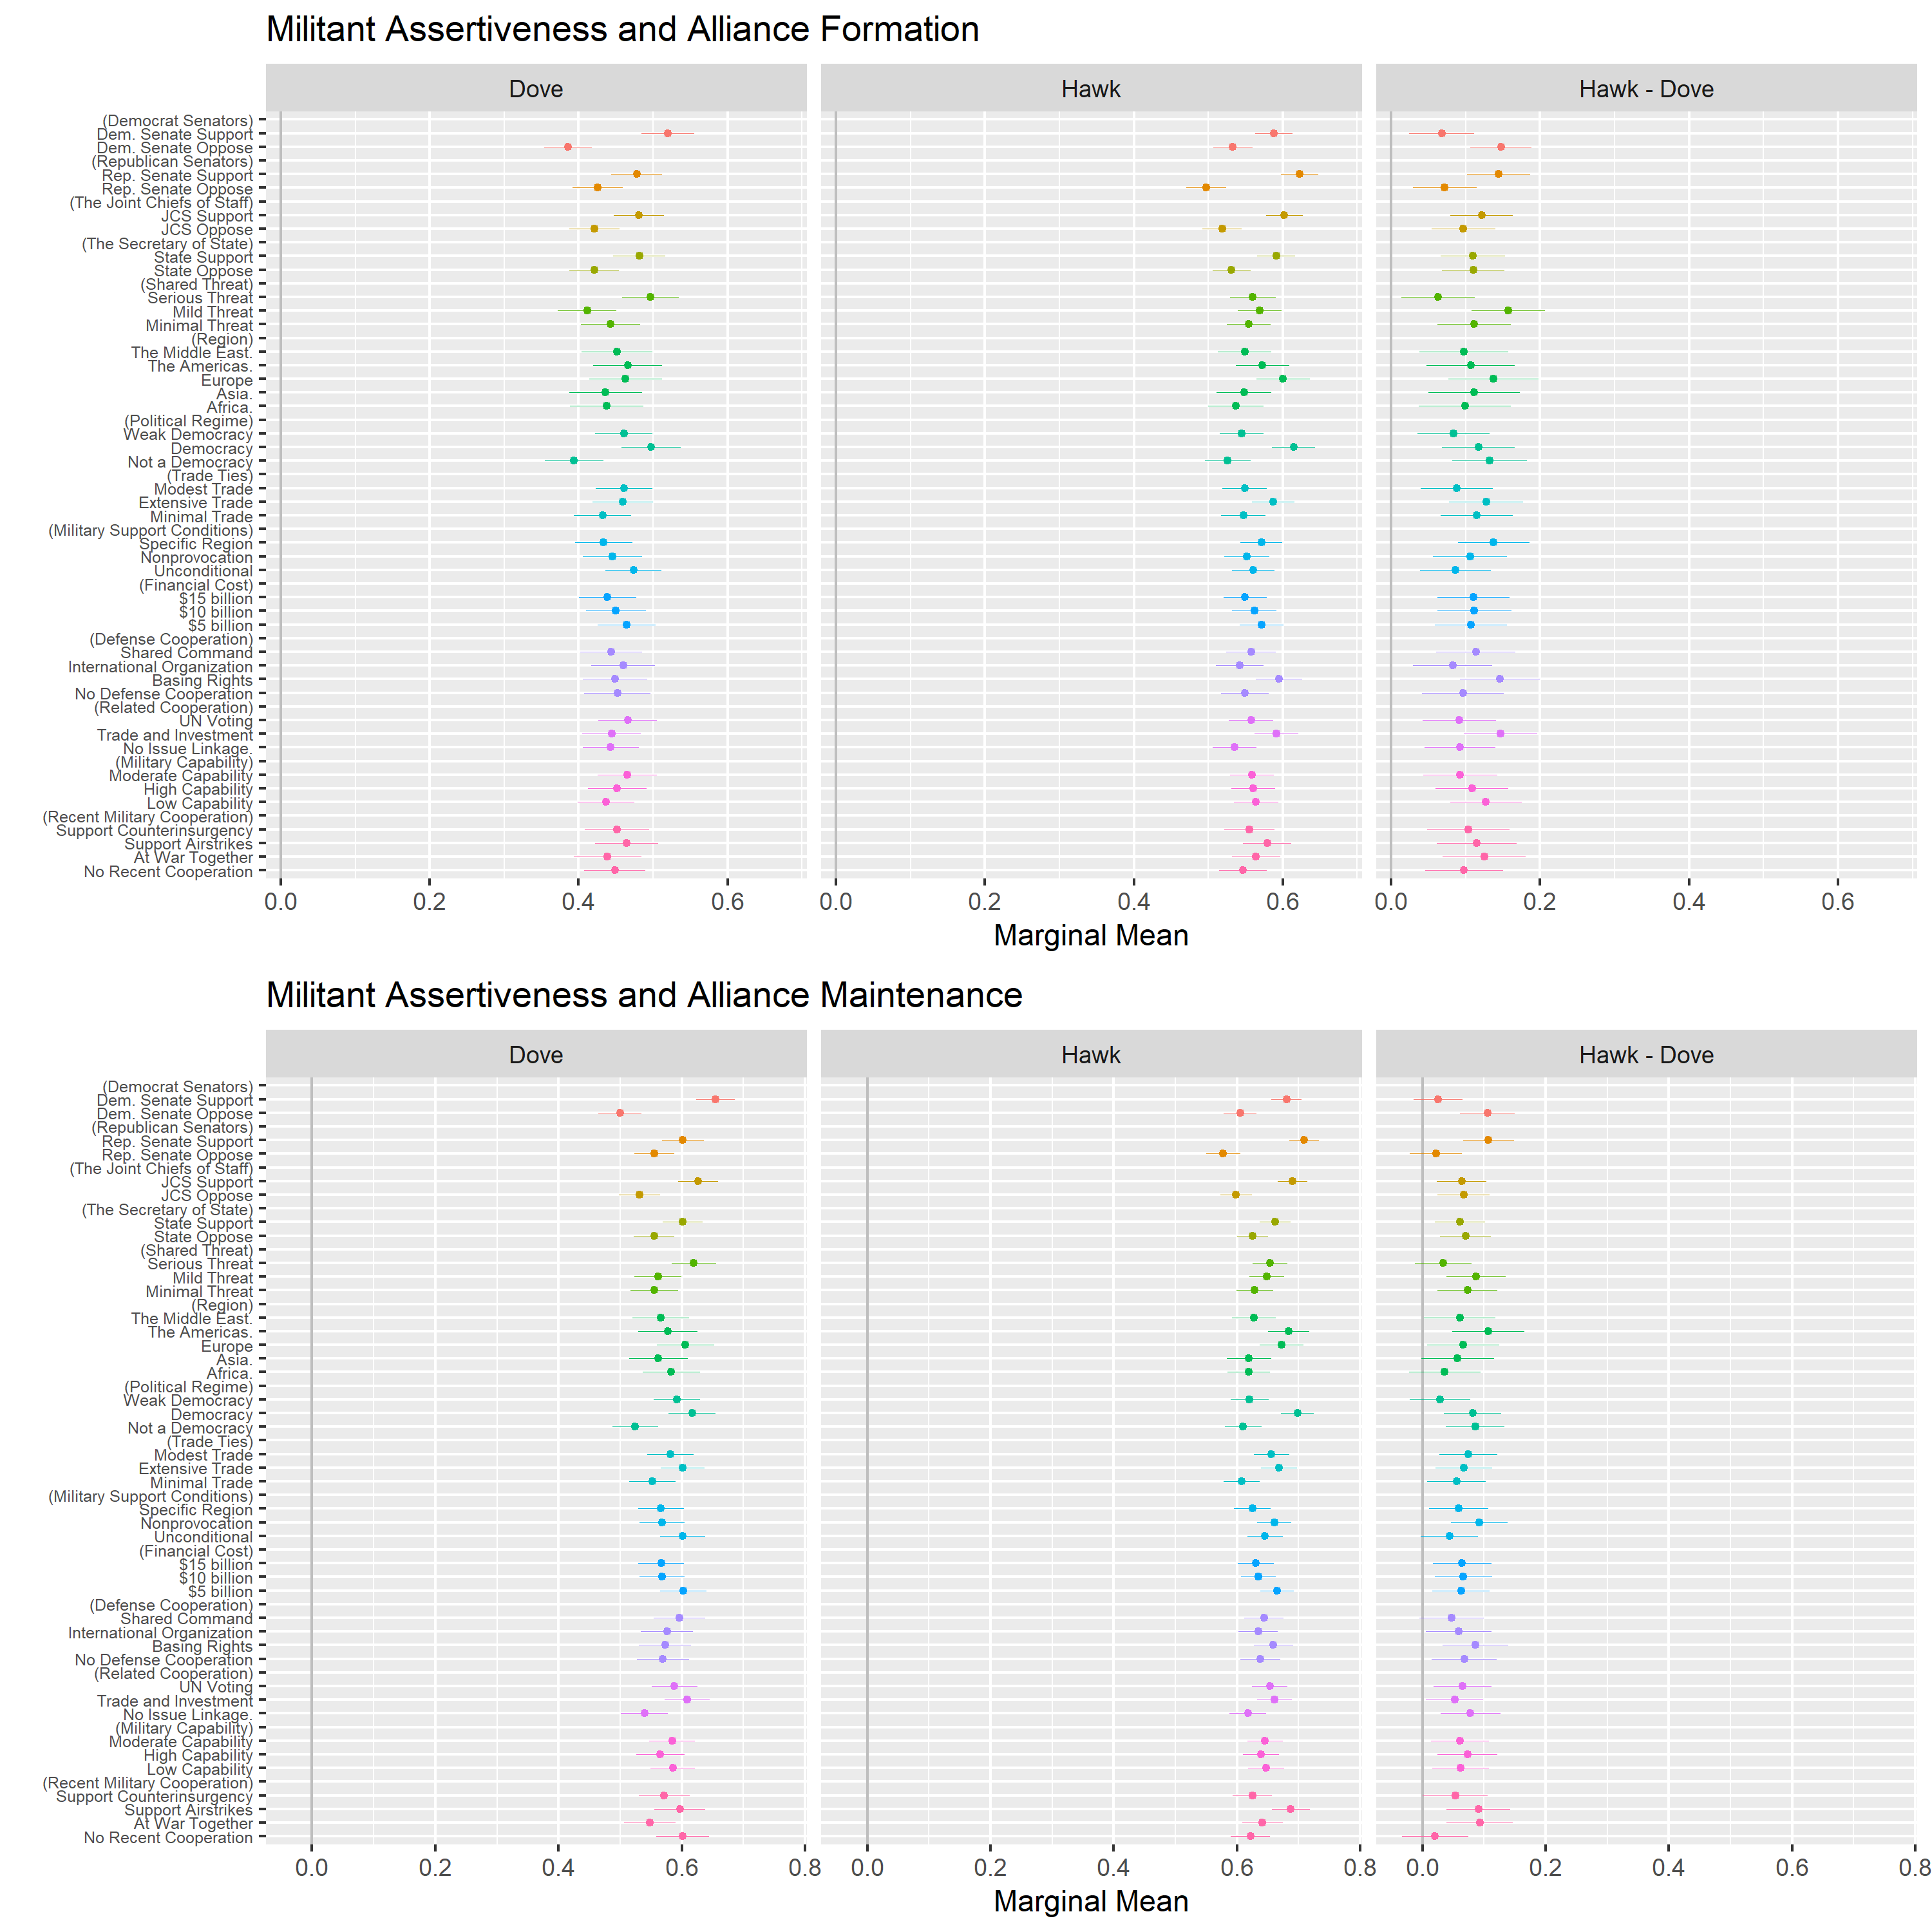
\includegraphics[width=0.95\textwidth]{hawk-plots.png}
	\caption{Marginal means of support for forming or maintaining a hypothetical alliances by militant assertiveness. For each experiment, the left two panels plot the marginal mean of support for alliance participation among hawks and doves under different alliance treatments. The rightmost panel plots the difference between these groups. Components marked with abbreviated labels and some attributes omitted to make the plot more legible.}
	\label{fig:hawk-plots}
\end{figure}


\begin{figure}
	\centering
		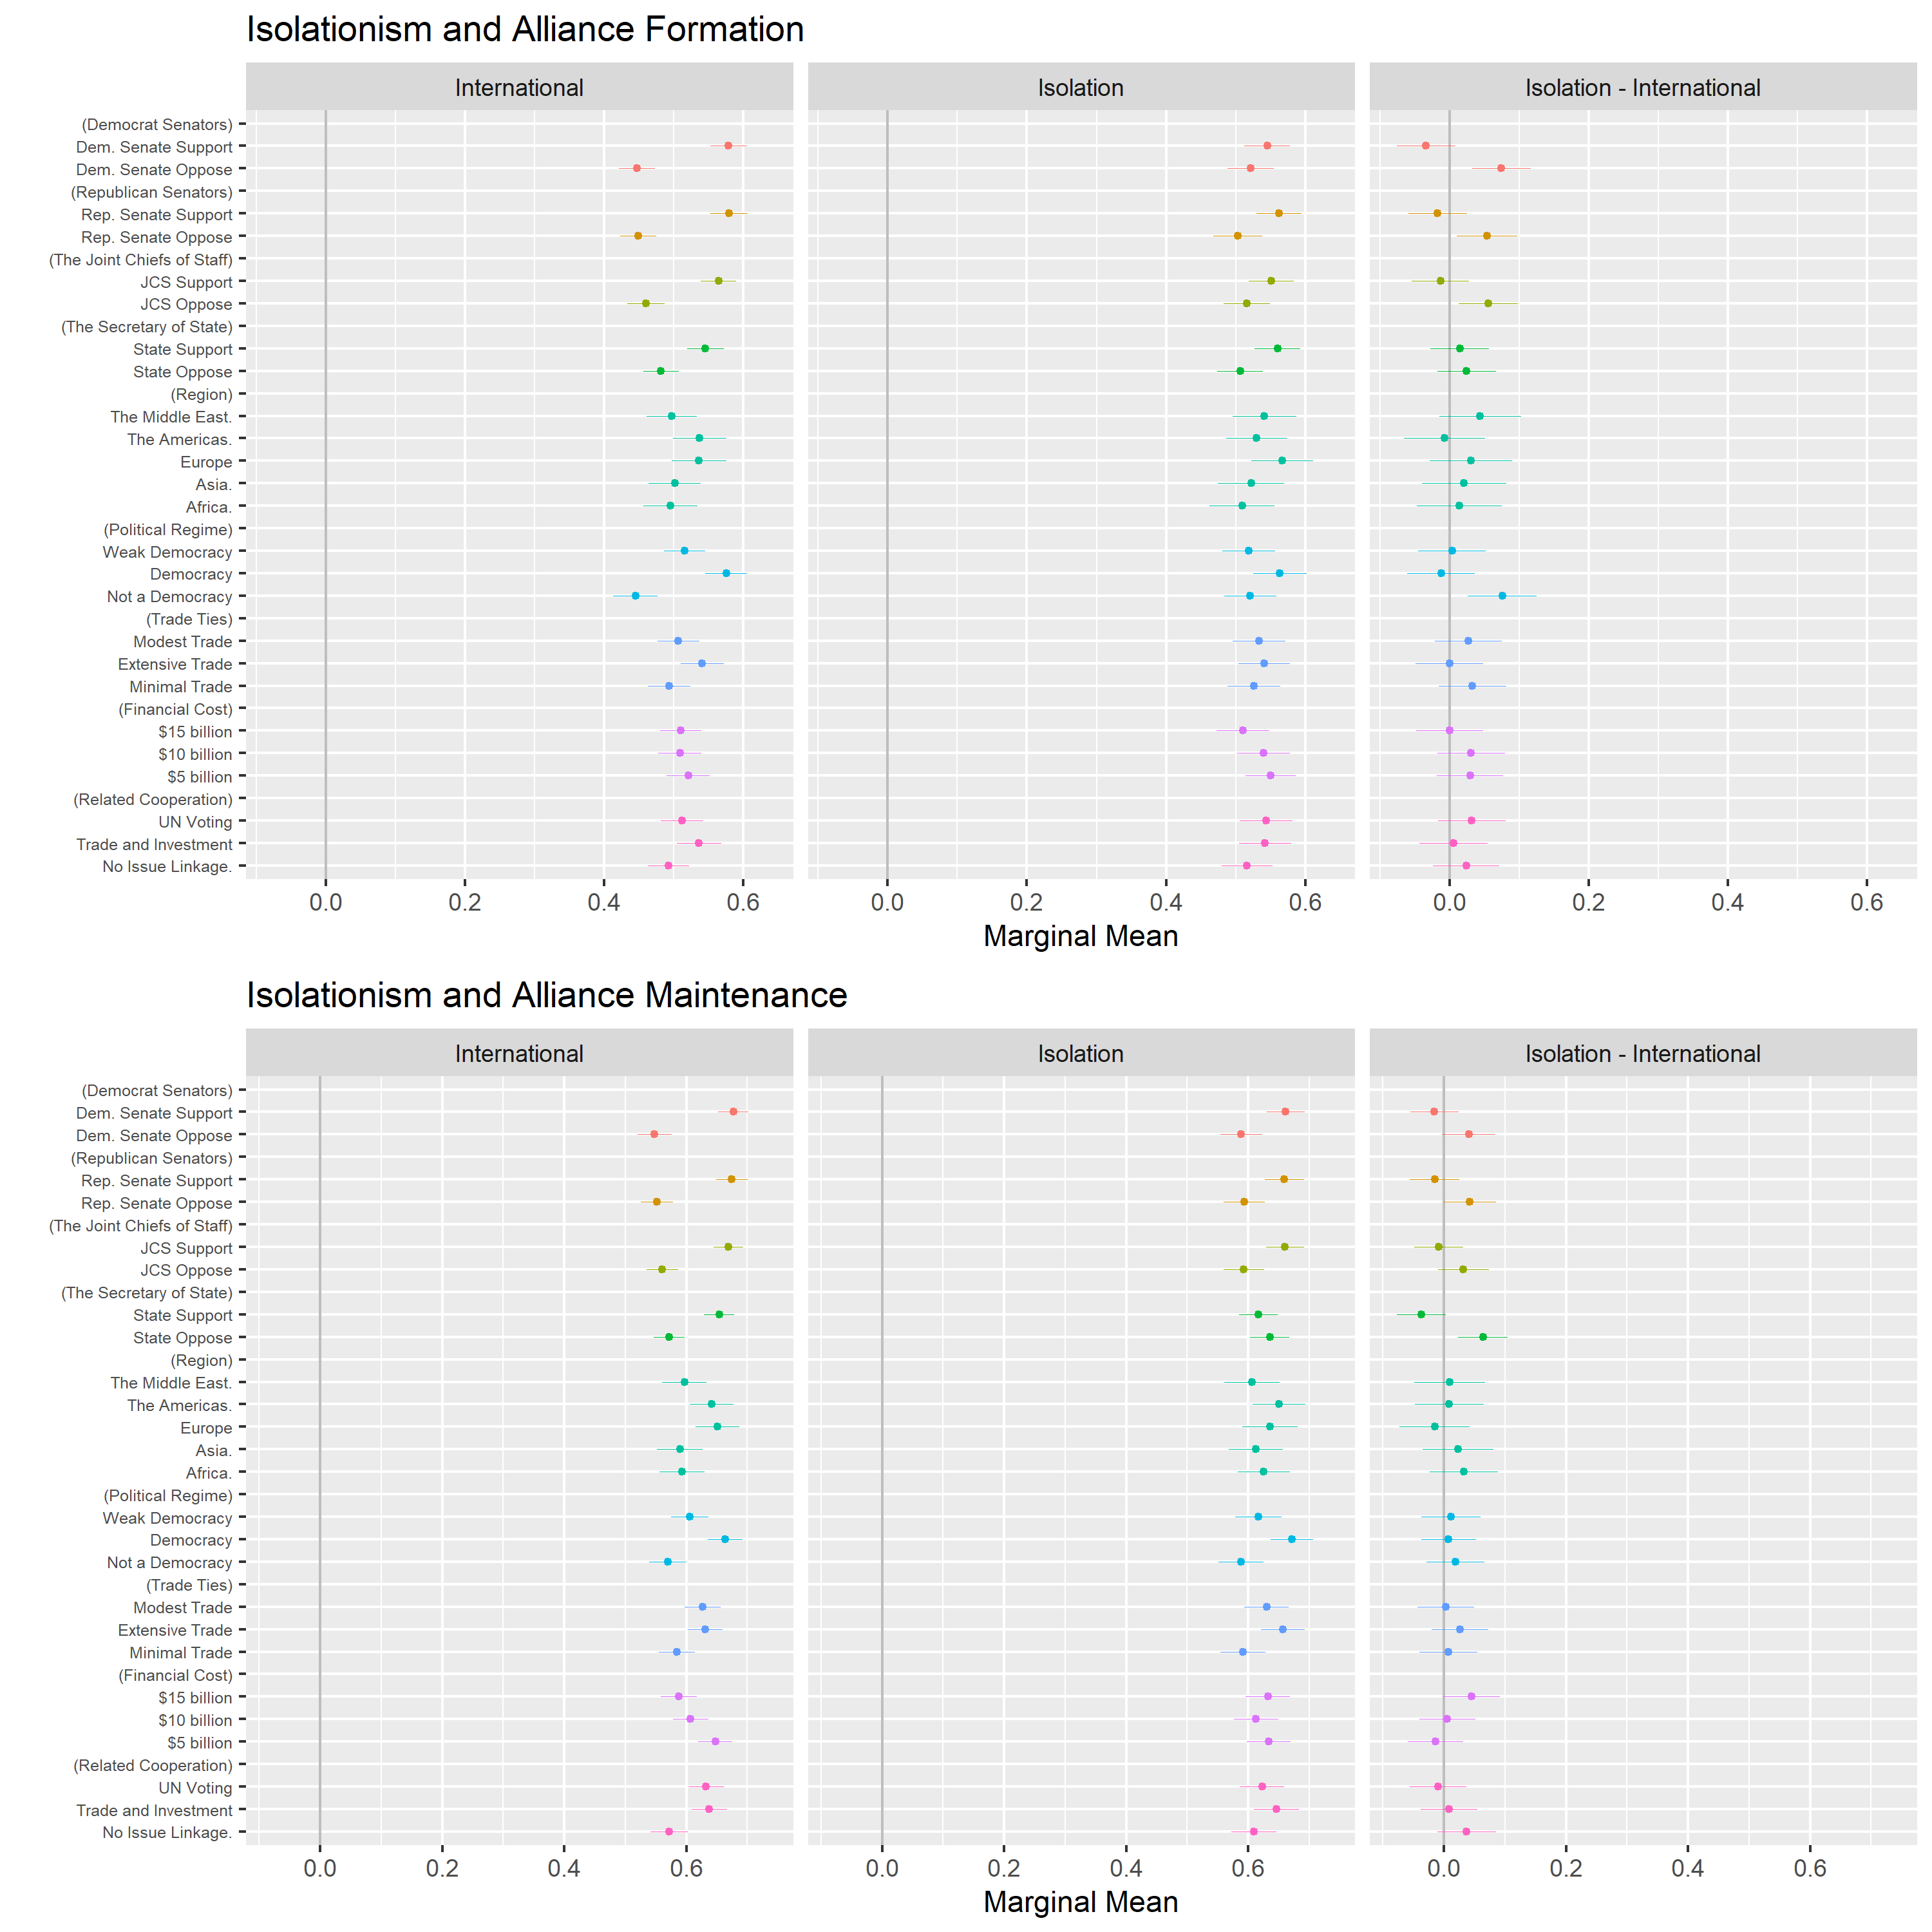
\includegraphics[width=0.95\textwidth]{isolation-plots.png}
	\caption{Marginal means of support for forming or maintaining a hypothetical alliances by internationalism. For each experiment, the left two panels plot the marginal mean of support for maintaining an alliance among isolationists and internationalists under different alliance treatments. The rightmost panel plots the difference between these groups. Components marked with abbreviated labels and some attributes omitted to make the plot more legible.}
	\label{fig:isolation-plots}
\end{figure}


Isolationism does not reduce baseline support for alliances, but it affects individual responses to elite cues. 
Internationalist respondents are more receptive to elite cues, as \autoref{fig:isolation-plots} shows. 
Although isolationists and internationalists express similar support for alliance participation across most alliance attributes, support among internationalists diverges strongly in response to elite cues. 
As a result, isolationists sometimes express higher alliance support than internationalists when elites oppose treaty formation. 
This highlights the importance of examining partisanship, isolationism and militant assertiveness at the same time. 




\newpage 



\section{Partisan Differences in Alliance Attitudes}

This section considers partisan differences in alliance attitudes without dividing by foreign policy dispositions. 
It also summarizes the alliance attitudes of independents who expressed no partisan lean. 
\autoref{fig:joint-part-plots} plots the marginal means of alliance support among Democrats, independents, and Republicans, along with the estimated differences in marginal means between these groups. 


Democrats and Republicans respond primarily to copartisan elites.
Support for new and existing alliances is much higher among Democrats when Democratic Senators support the alliance.
Similarly, Republicans follow cues from Republican Senators.


There are other clear partisan differences in alliance attitudes.
Democrats are more likely to support alliance formation and maintenance regardless of alliance characteristics, relative to Republicans. 
Independents match Republicans in their attitudes towards alliance maintenance, but they are even more skeptical of forming new treaty commitments. 


Independents are more likely to support alliances with backing from Republican Senators, but otherwise are less responsive to alliance characteristics and elite cues. 
As a result, there are substantial differences between the three partisan groups. 
An omnibus F-test finds significant differences between models that interact partisanship and the various treatments with unconditional models of alliance formation and maintenance. 


\begin{figure}
	\centering
		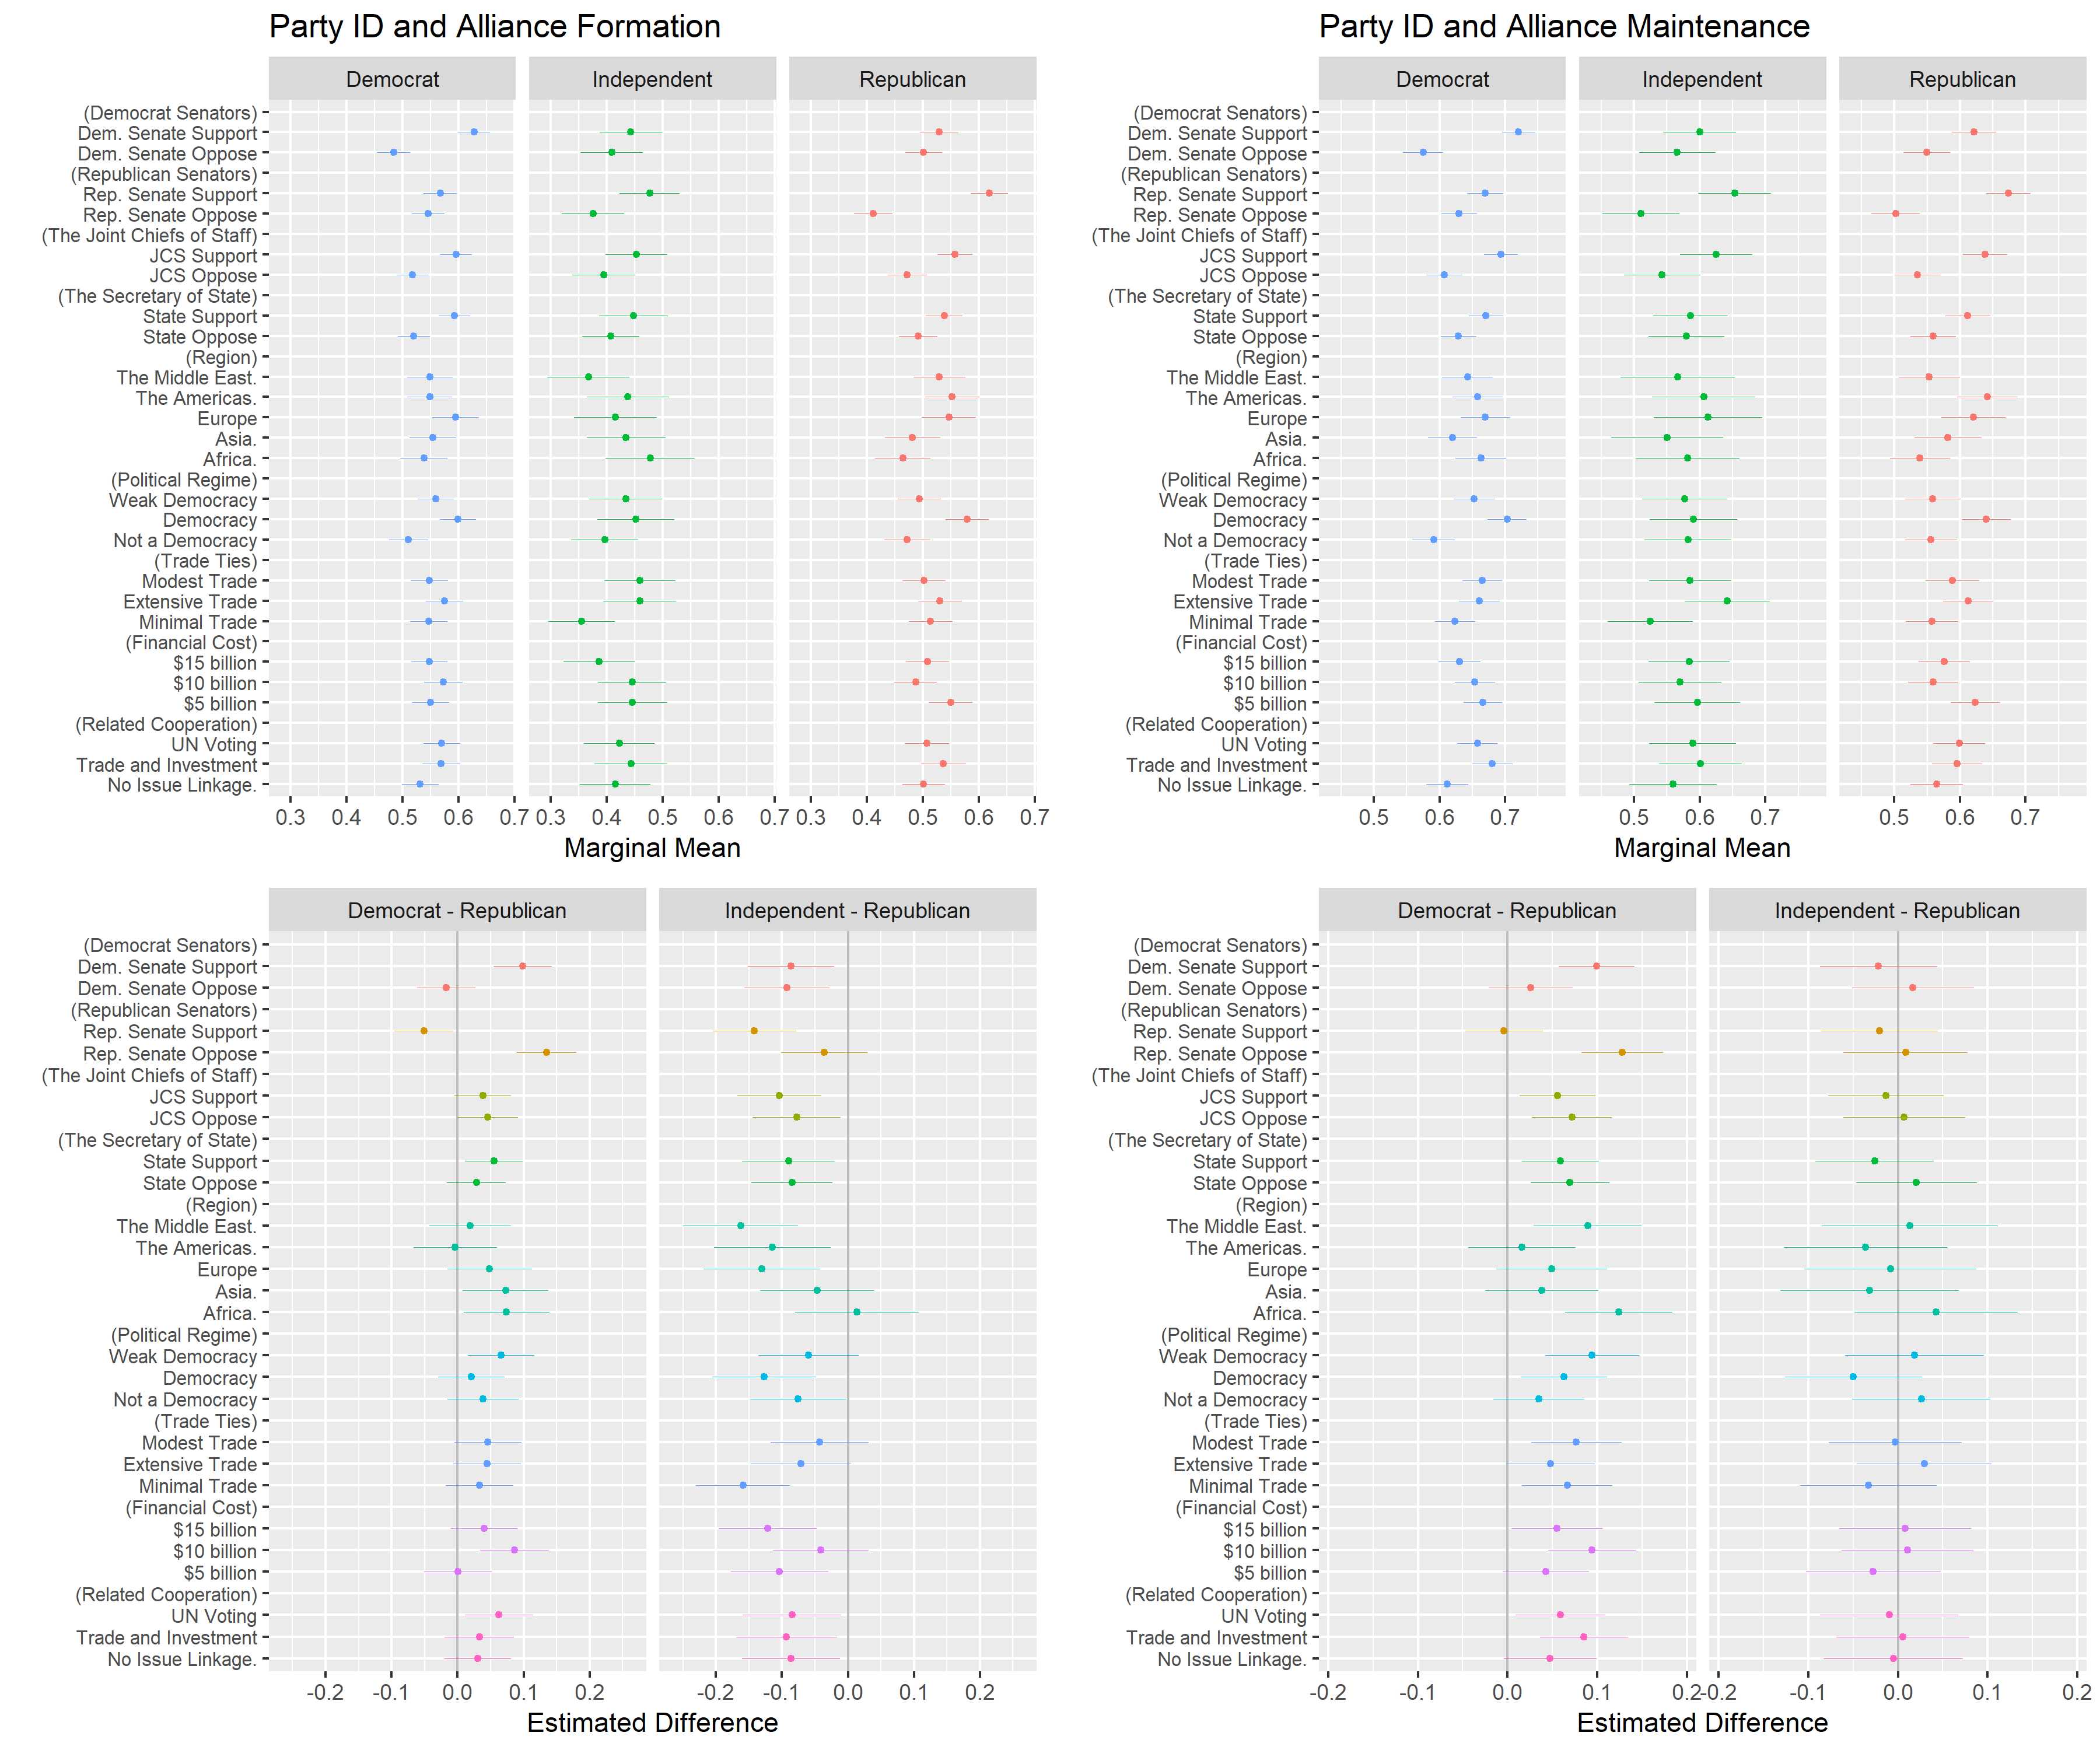
\includegraphics[width=0.95\textwidth]{joint-part-plots.png}
	\caption{Marginal means of support for forming or maintaining a hypothetical alliances by partisanship. For each experiment, the left two panels plot the marginal mean of support for maintaining an alliance among Democrats and Republicans under different alliance treatments and the rightmost panel plots the difference between these groups. Components marked with abbreviated labels and some attributes omitted to make the plot more legible.}
	\label{fig:joint-part-plots}
\end{figure}


Besides elite cues, there are other salient differences in how partisans respond to alliance attributes.
Established democracy in an ally increases Republican support, but allied democracy exerts more influence on Democrats, who also prefer alliances with weak democracies to non-democratic allies. 
These partisan differences in attitudes towards allied democracy are less pronounced in the alliance formation experiment, however. 


There is also a noteworthy partisan divide in attitudes towards alliances in different regions.
Republicans are less likely to support new or existing alliances with African countries. 
Existing Middle Eastern and new Asia alliances also receive lower support from Republicans than Democrats.
The source of these differences merit further investigation. 
Perhaps Republican ethnocentrism has some role in regional alliance preferences. 


Overall, \autoref{fig:joint-part-plots} reveals clear partisan differences in alliance attitudes. 
Members of the two major parties follow cues from co-partisan elites and value different alliance characteristics. 
These differences are consistent with the findings in the manuscript, as they reflect aggregate attitudes across the varying foreign policy dispositions within each party. 



\section{Open-Ended Alliance Attitude Question} 


To further examine the sources of alliance attitudes, I asked respondents to identify the most important factors behind their support or opposition to the hypothetical alliances in an open-ended question. 
Roughly half of the respondents gave an invalid response, which limits the utility of the following analysis. 
The results do provide some insight into the individual characteristics that predict particular emphases in alliance attitudes, however. 


Based on the open-ended question responses, I created three dummy indicators. 
The first takes on a value of one if an individual mentions any of the following; generic elite cues, bipartisanship, partisan leaders, military leader support, or diplomatic elite cues. 
The second has a value of one if a respondent references alliance partner attributes such as trade, regime type, threat, region, recent military cooperation and capability. 
The last dummy indicator captures any mention of alliance obligations, including cost, issue linkages, defense cooperation and conditions on military support. 
These three variables are not mutually exclusive, because some respondents mentioned multiple factors from different categories. 


Because individuals highlight multiple alliance attributes, I analyze the open-ended responses with a trivariate probit model, which adjusts for correlations between the different response classes. 
Each equation of the model predicts open-ended response content using individual characteristics, including the strength of individual partisan attachment, international economic interests, gender, race, education, region and income. 
To ensure that the coefficient magnitudes are comparable, I rescaled all continuous variables by two standard deviations \citep{Gelman2008}. 
I estimated the trivariate probit model using the Joint Generalized Regression estimator of \citet{Braumoelleretal2018} and fit separate trivariate probit models for each experiment.\footnote{The pre-analysis plan stated that I would use Bayesian estimation of the multivariate probit model. Unfortunately, this proved impractical, as the Bayesian model would not converge and was numerically unstable. This also precluded a more fine-grained analysis with more response categories.} 


\begin{figure}
	\centering
		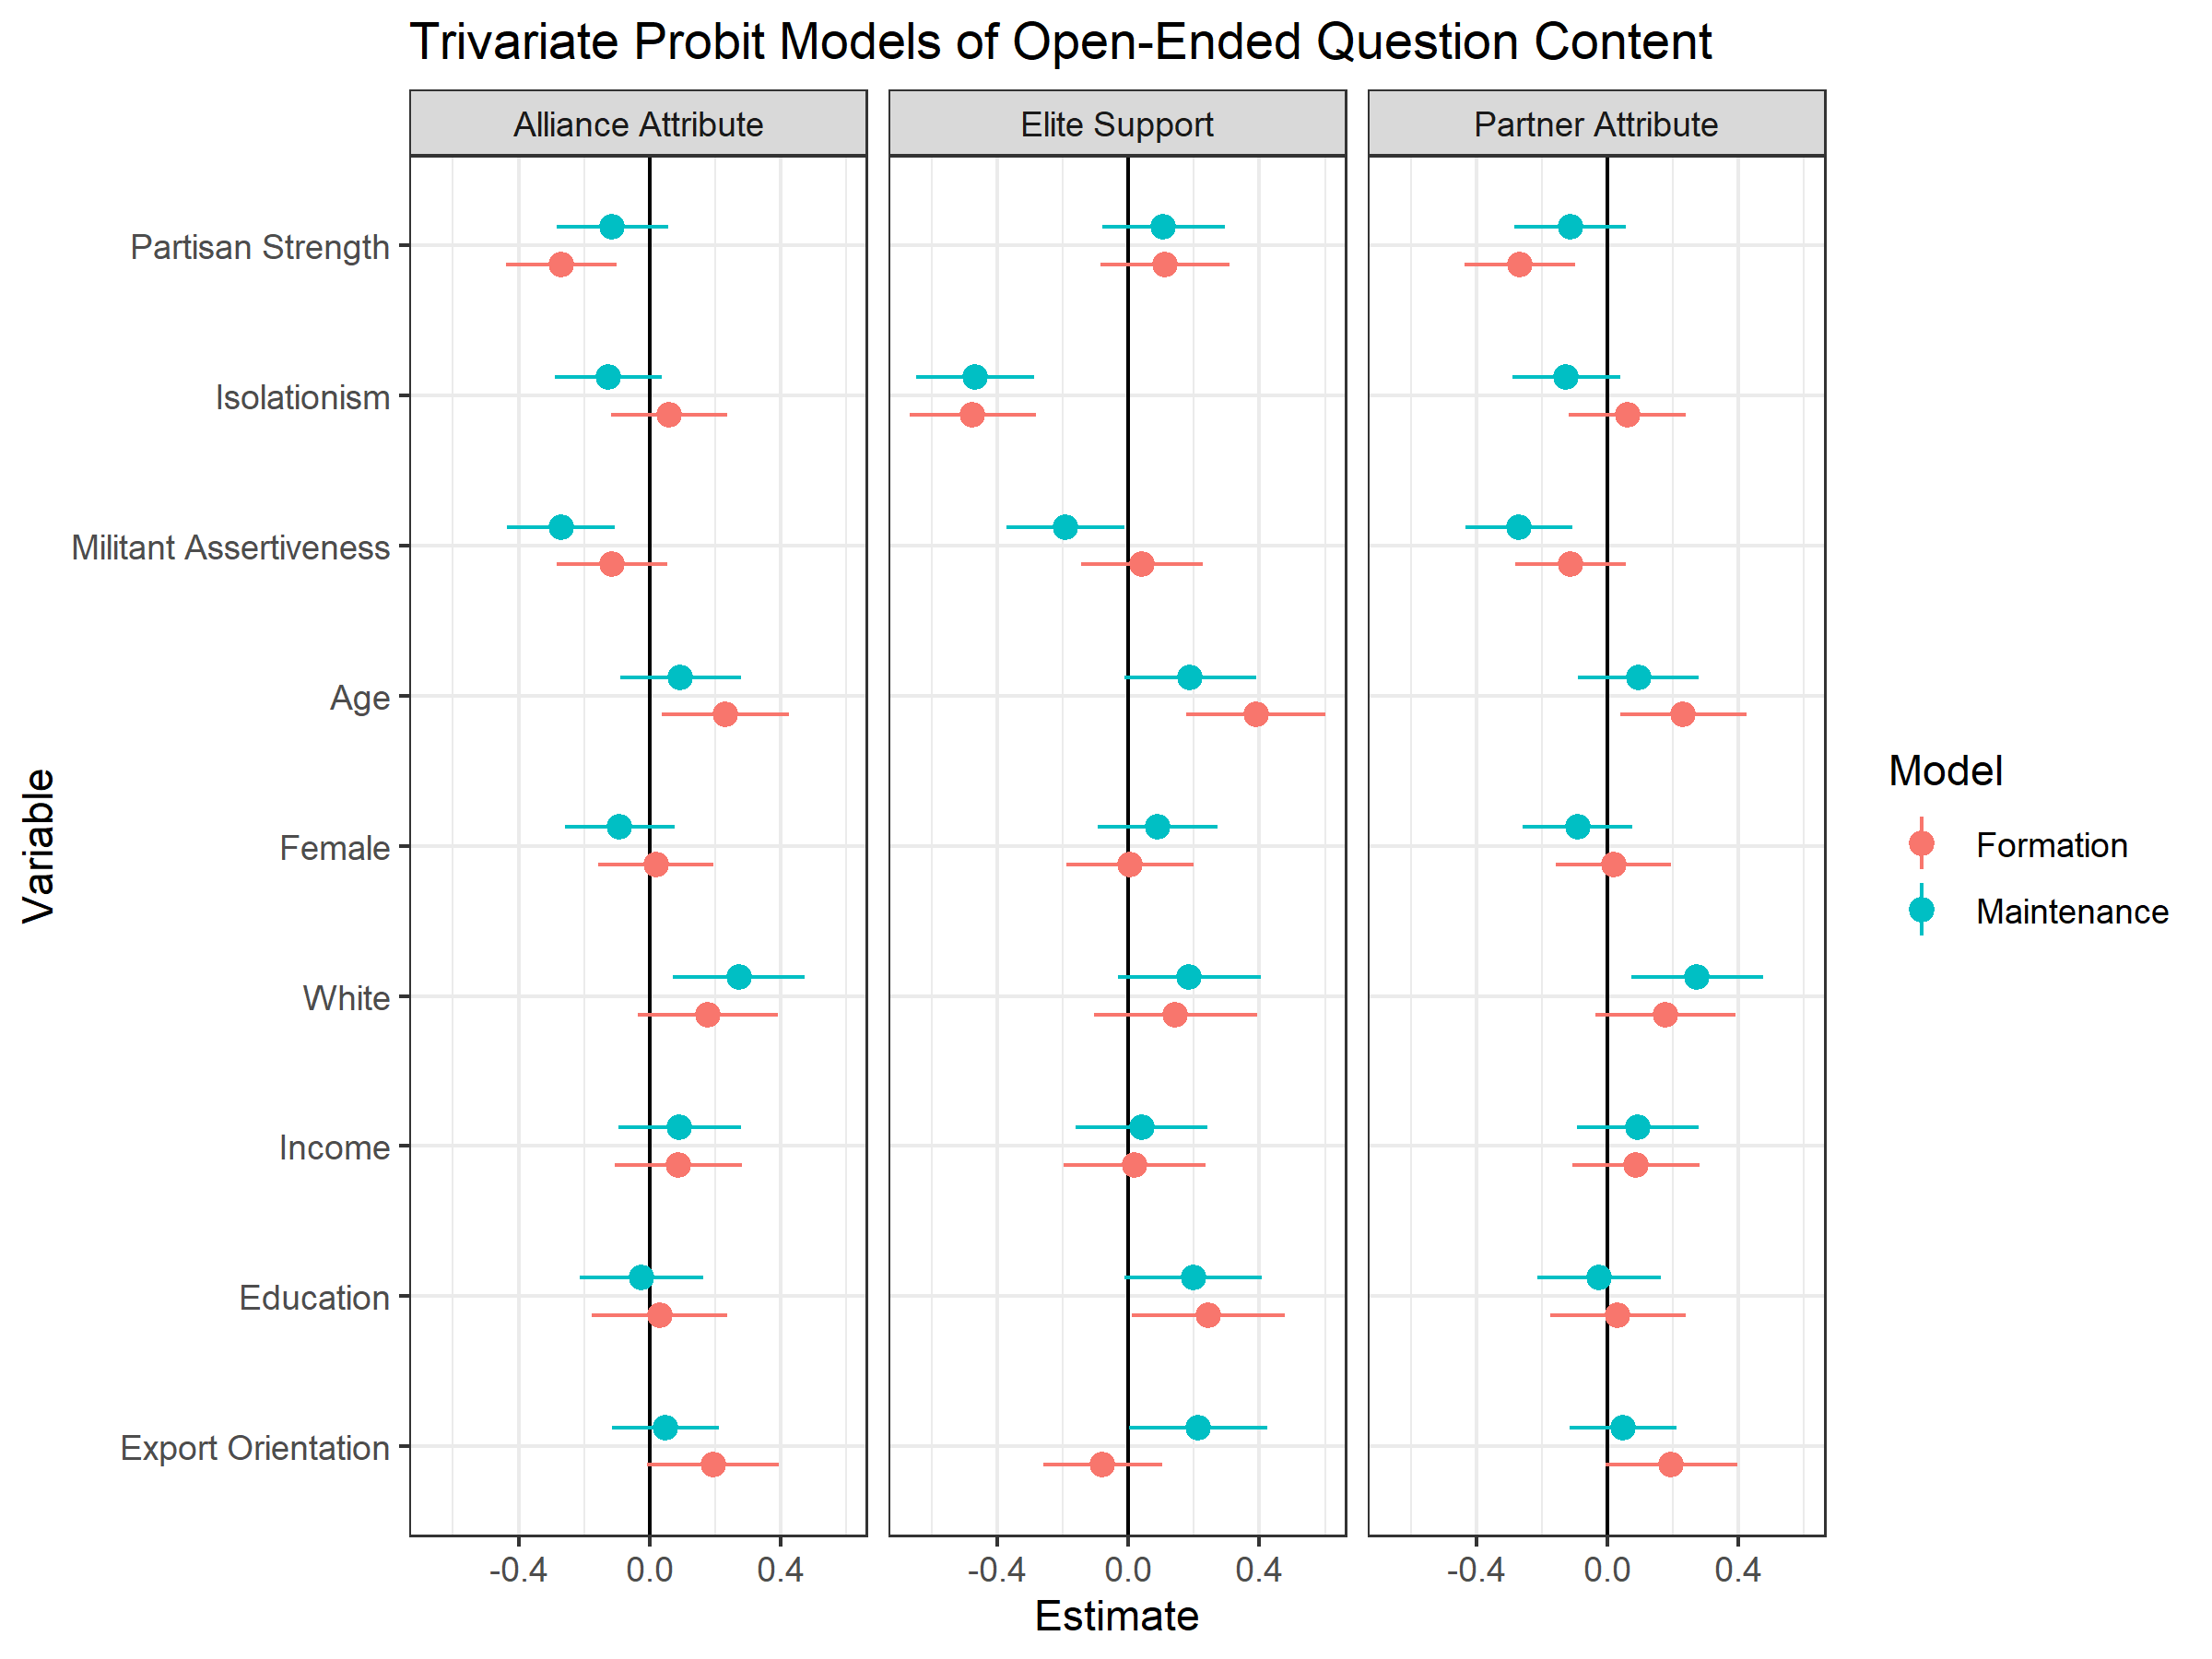
\includegraphics[width=0.95\textwidth]{open-questions-res.png}
	\caption{Coefficient estimates from trivariate probit models of open-ended response content in the alliance formation and maintenance experiments. Panels show the coefficients for each equation, points mark the coefficient estimates, and error bars capture the 95\% confidence intervals. Colors differentiate between the formation and maintenance experiments. All continuous variables rescaled by two standard deviations.}
	\label{fig:openq-res}
\end{figure}



I plot the probit coefficients for each equation of two models in \autoref{fig:openq-res}. 
These estimates of the relationship between indidividual concerns and open-ended response content reveal further patterns that are consistent with the results in the manuscript.
As isolationism increases, individuals are less likely to mention elite cues as a source of their responses.\footnote{Two respondents in the formation experiment explicitly called themselves isolationists.} 
Isolationism has the largest substantive effect. 
Hawkish individuals are less likely to mention any treatment, especially in the maintenance experiment, which may reflect high alliance support regardless of the alliance profile.
This reflects hawks' tendency to express strong alliance support regardless of experimental treatments.  
Last, stronger partisan attachment makes individuals less likely to mention alliance or partner attributes. 


There are a few other noteworthy patterns.
Greater education is positively correlated with mentioning elite support. 
A two-standard deviation increase in age also increases the likelihood of mentioning all three factors. 
Individuals with economic ties to export-oriented sectors follow elites on alliance maintenance, but pay more attention to partner and alliance attributes in alliance formation. 


\newpage


\section{Ratings Results}

In the two experiments, I ask respondents to answer yes or no on alliance formation or maintenance and provide a numeric rating of the alliance. 
Ratings range from zero to 100, where 0 is a poor alliance and 100 is a great alliance. 
This section of the appendix compares the choice and rating results. 
Although the choice outcome reflects more common survey questions and substantive concern, the rating measure has a more intuitive interpretation. 
To do this, \autoref{fig:formation-plots} and \autoref{fig:maintenance-plots} plot the unconditional AMCE estimates for the rating and choice measures in both experiments.  


\begin{figure}[htpb]
	\centering
		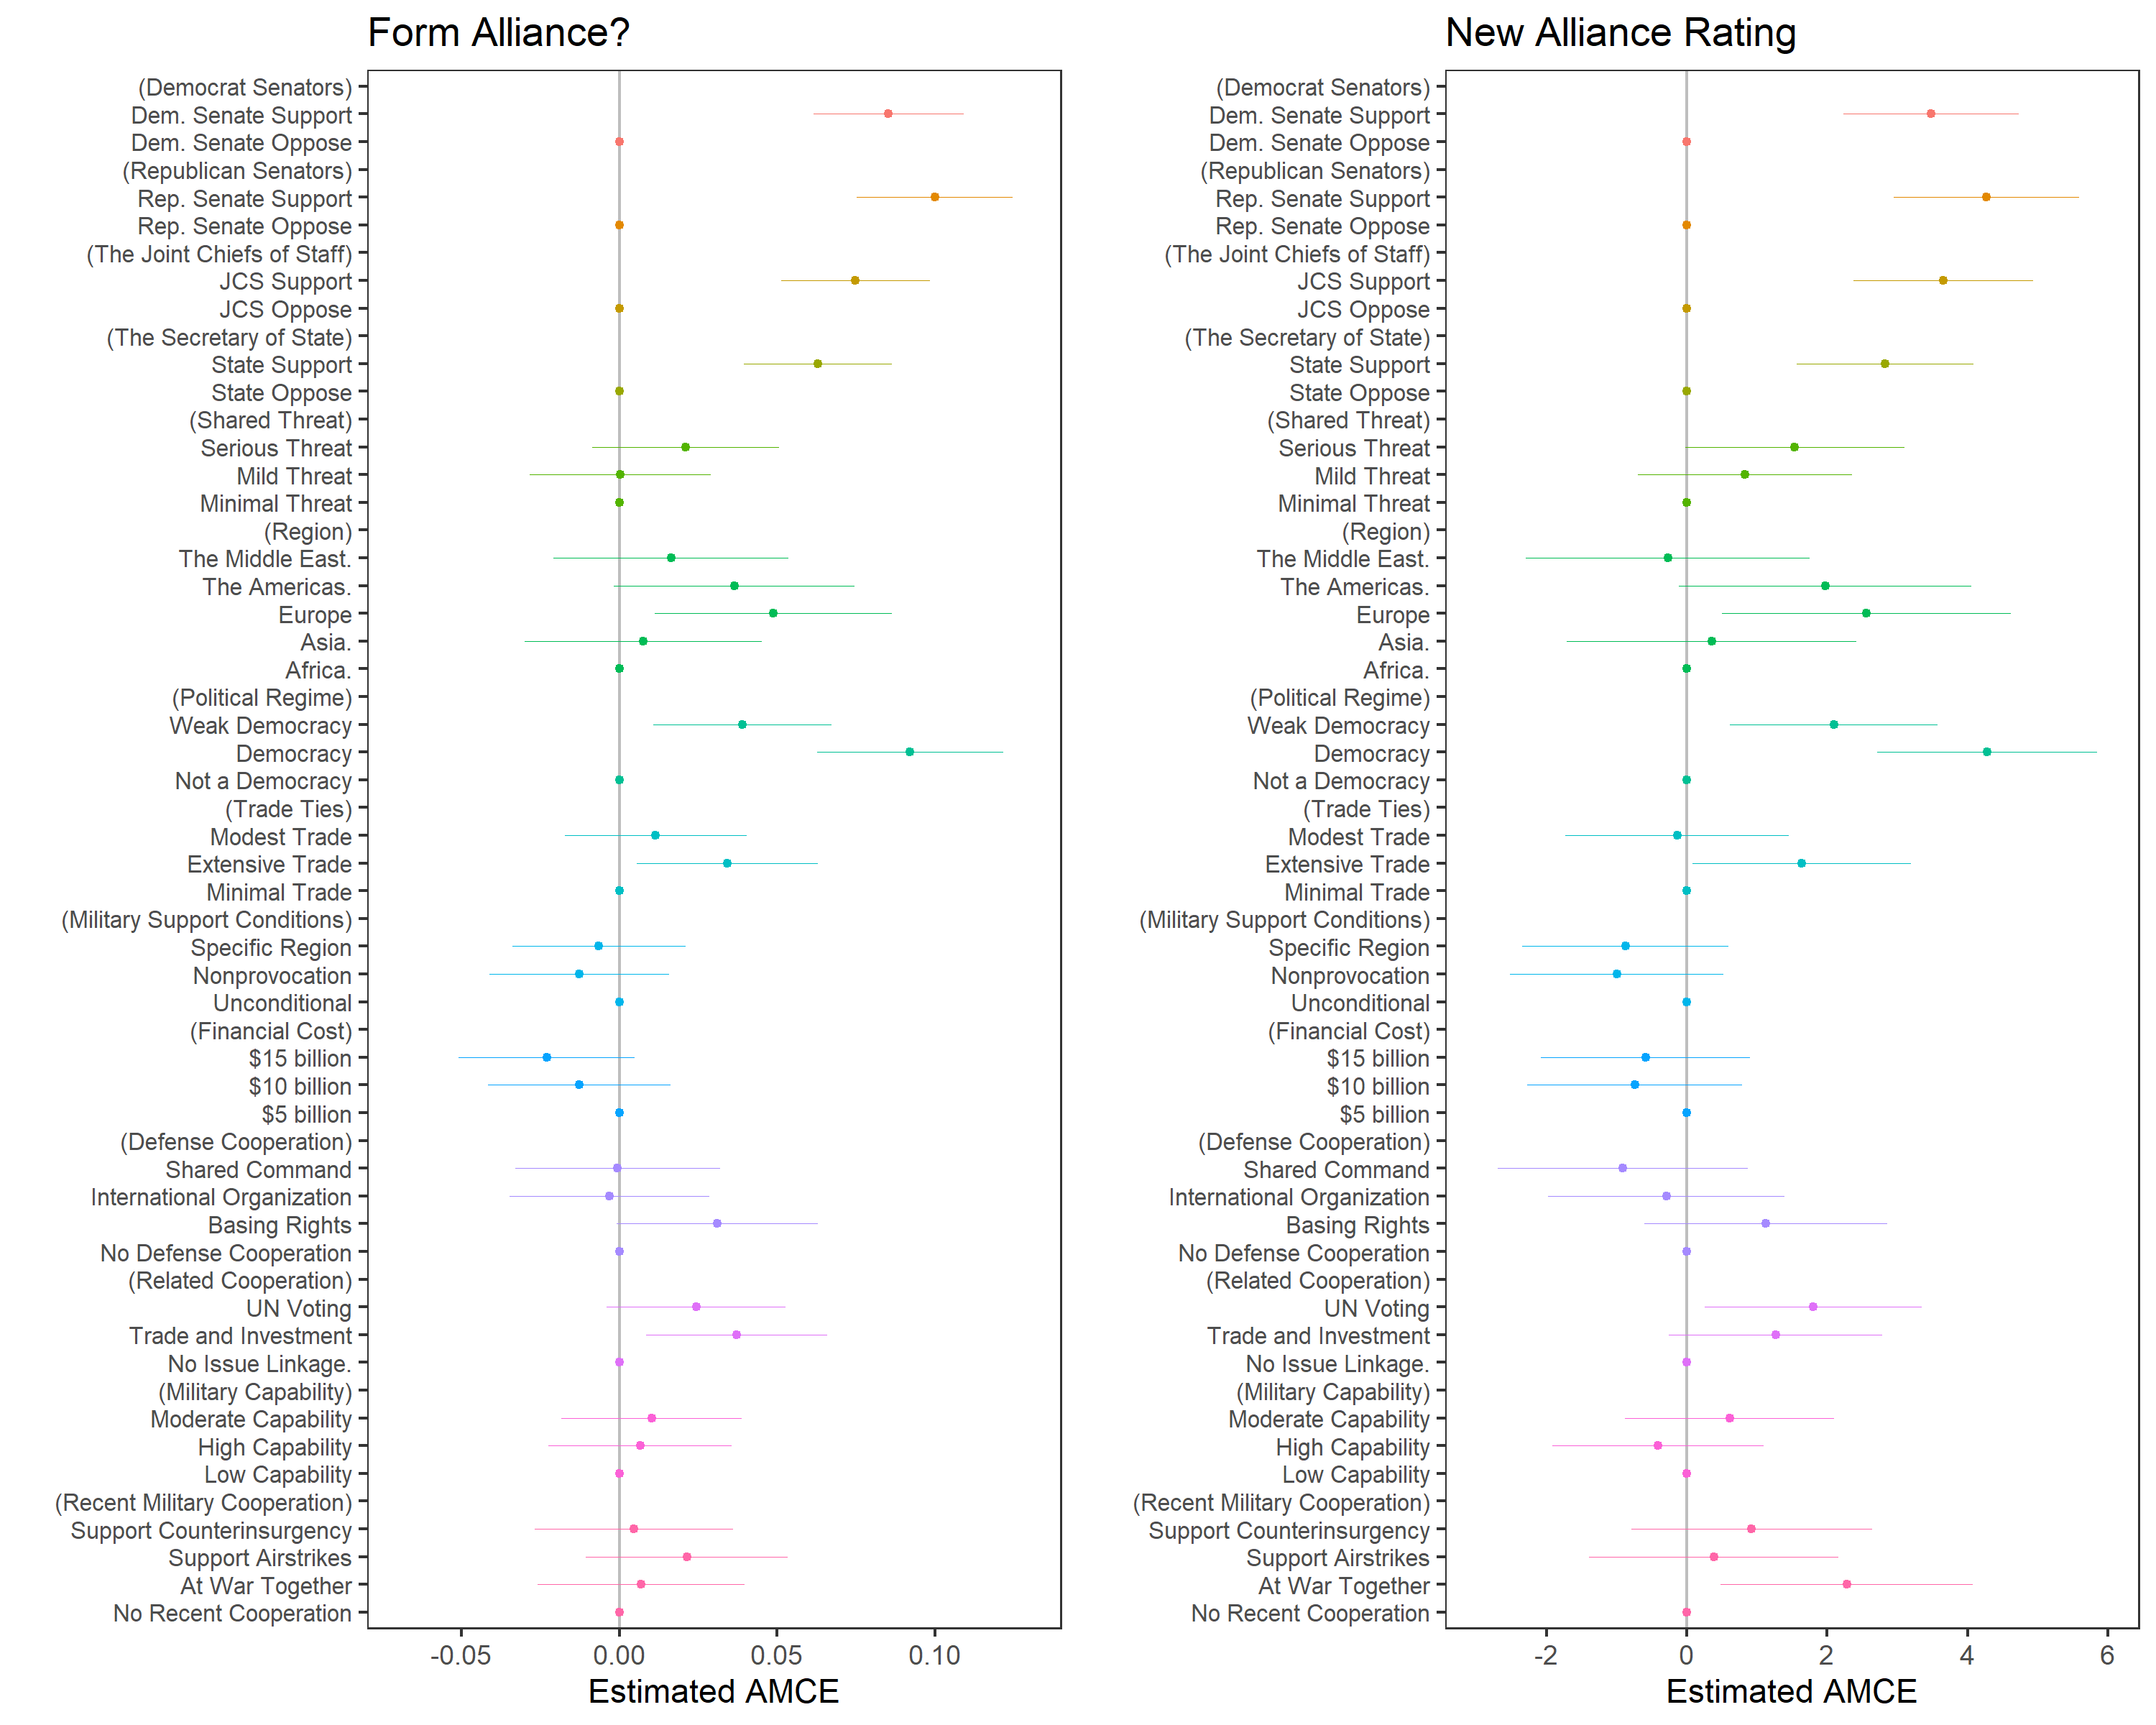
\includegraphics[width=0.95\textwidth]{formation-plots.png}
	\caption{Unconditional AMCE estimates for alliance formation choices and ratings.}
	\label{fig:formation-plots}
\end{figure}


Regardless of the outcome measure, I make similar inferences about treatment effects in the two conjoint experiments. 
Democracy and elite cues are the dominant influences on support for new and existing alliances. 
Inferences about other factors are also similar, with some exceptions. 


There are minor differences between the choice and ratings results. 
In the alliance formation experiment, past support in war from a prospective ally has a much stronger effect on ratings. 
For alliance maintenance, there is a substantial difference in ratings between alliances with an annual cost of \$15 billion, relative to \$10 billion. 
The ratings results also show more evidence of a small positive impact for defense cooperation and recent military cooperation. 



\begin{figure}[htpb]
	\centering
		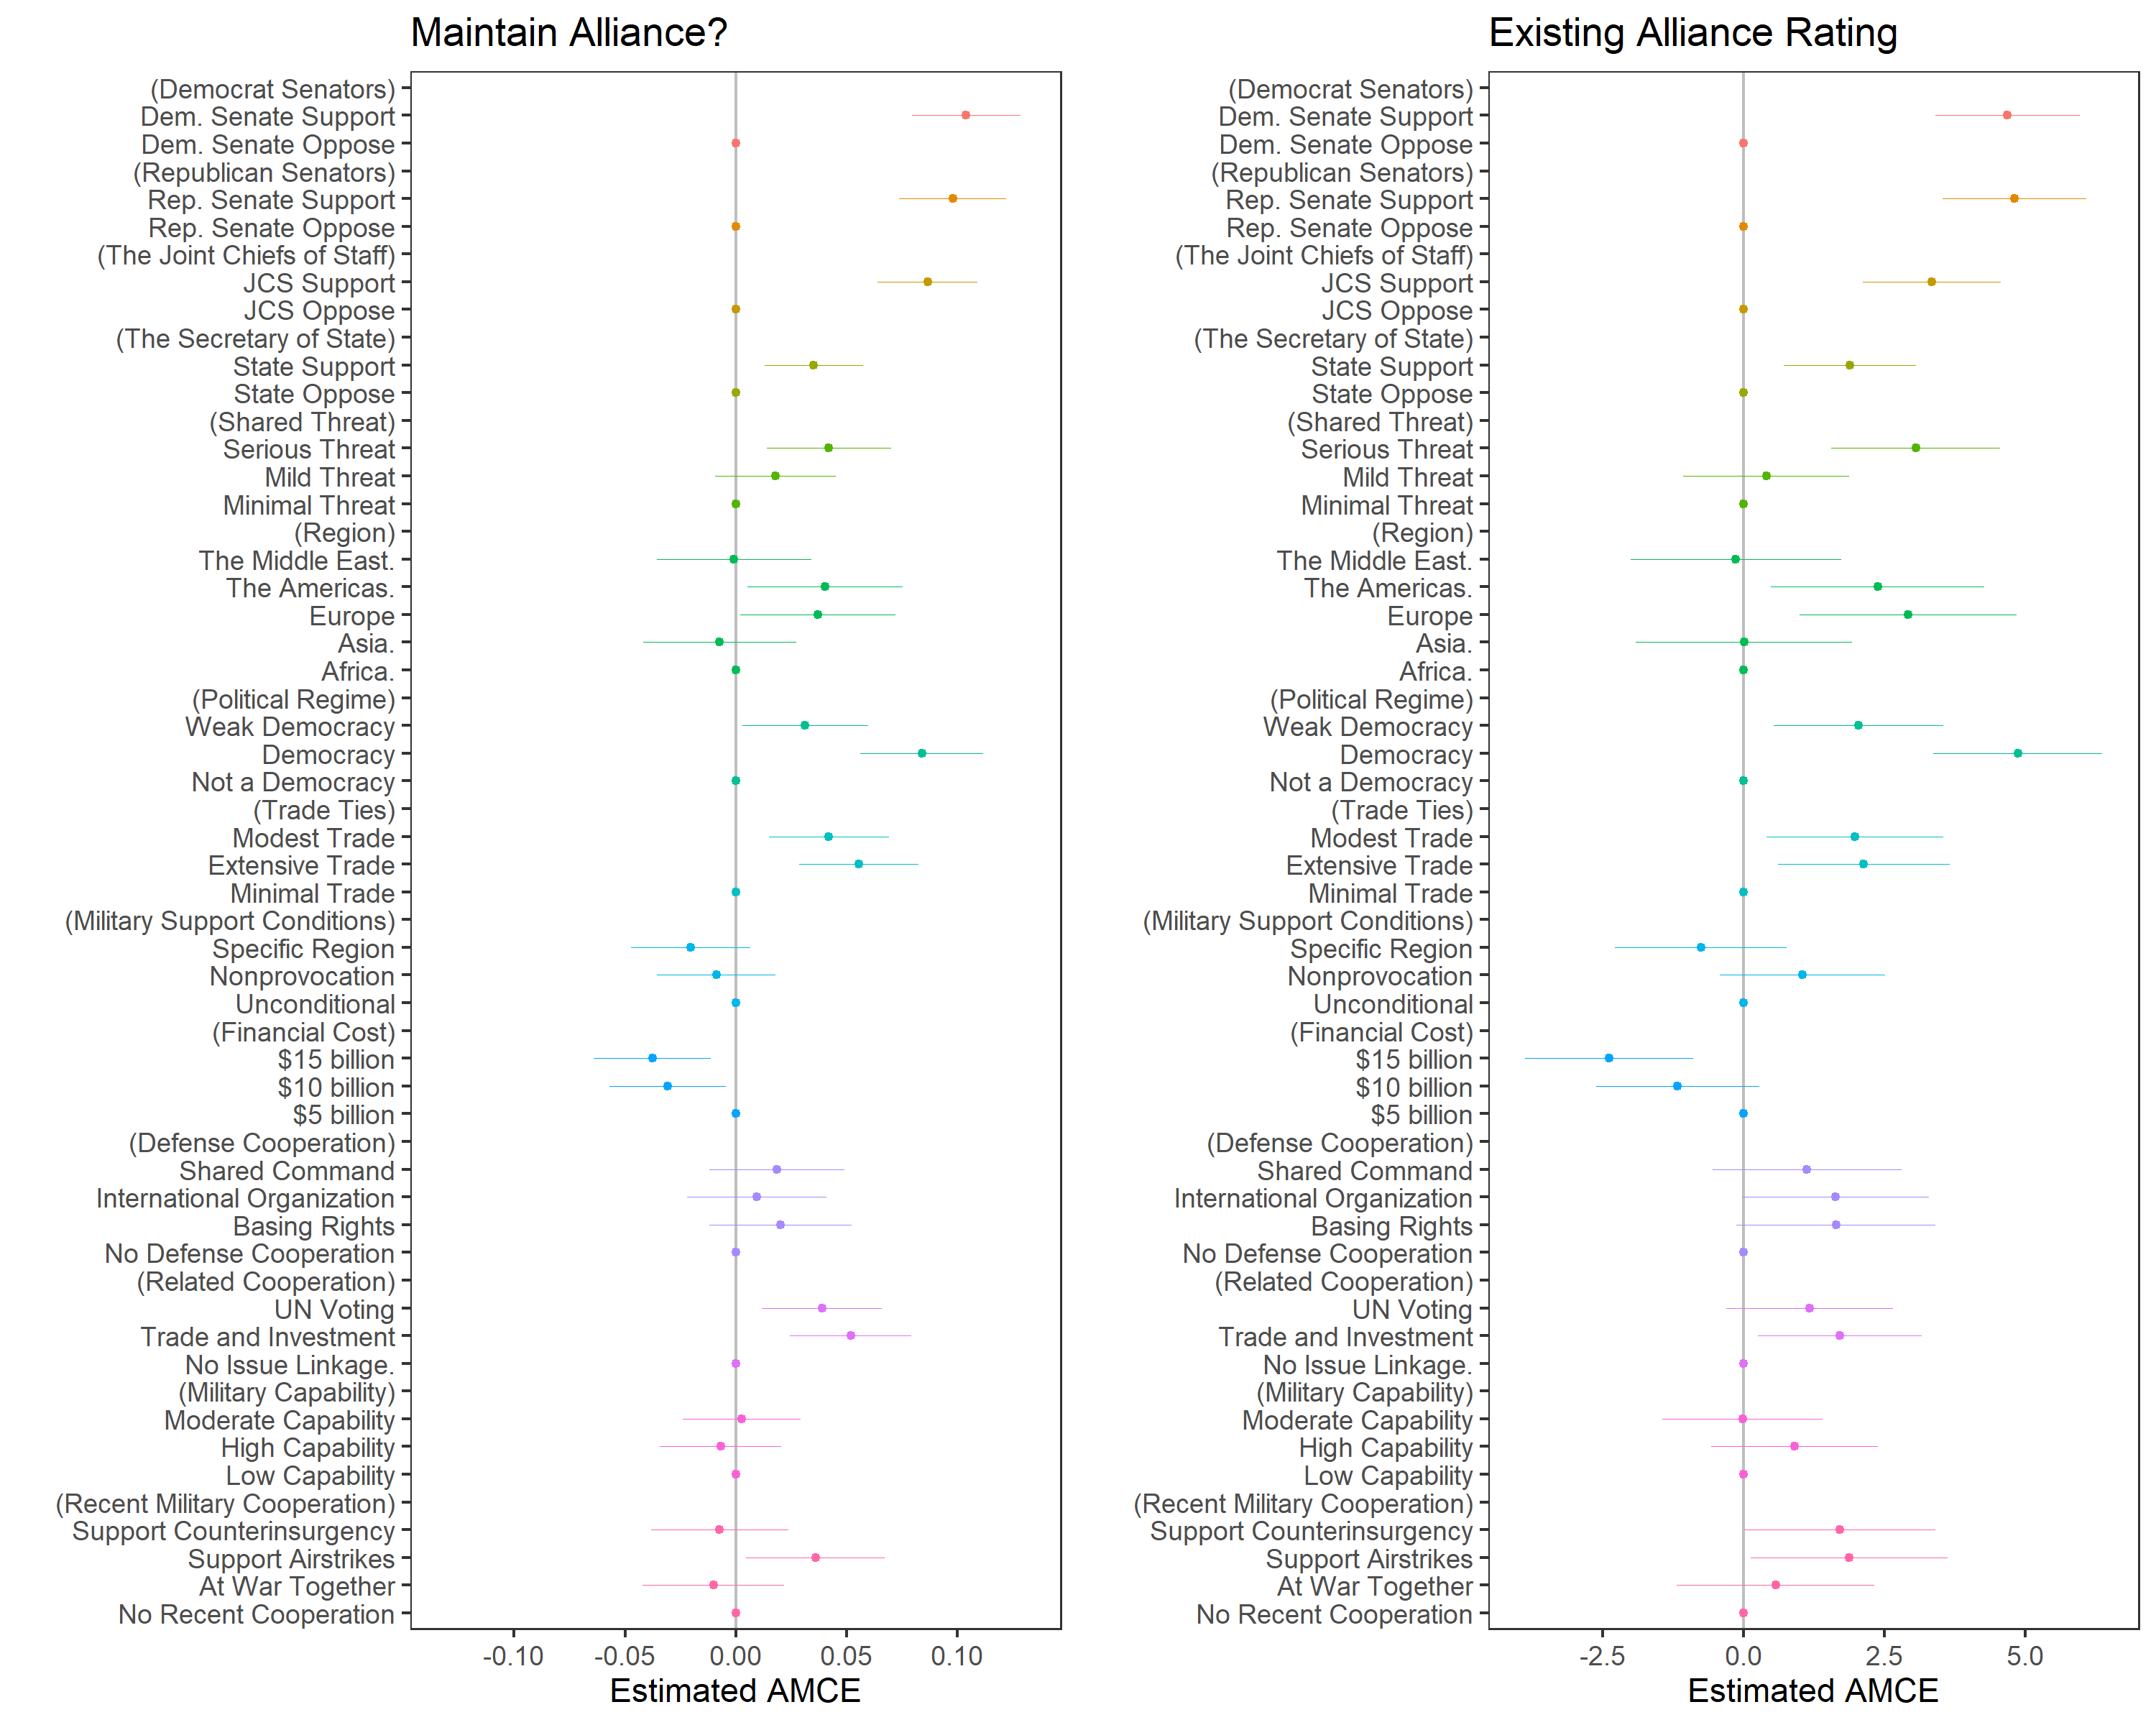
\includegraphics[width=0.95\textwidth]{maintenance-plots.png}
	\caption{Unconditional AMCE estimates for alliance maintenance choices and ratings.}
	\label{fig:maintenance-plots}
\end{figure}

%

On a scale from zero to 100, most factors have null or small effects. 
Only partisan elite cues and consolidated alliance democracy increase alliance ratings by more than three points. 


As with the choice measure, partisanship and foreign policy dispositions create substantial differences in alliance ratings under different elite cues.
\autoref{fig:party-dispo-form} and \autoref{fig:party-dispo-main} plot the marginal means of individual alliance ratings for elite cues across partisanship and foreign policy dispositions. 
The patterns in these figures are similar to the manuscript results.  


\begin{figure}[htpb]
	\centering
		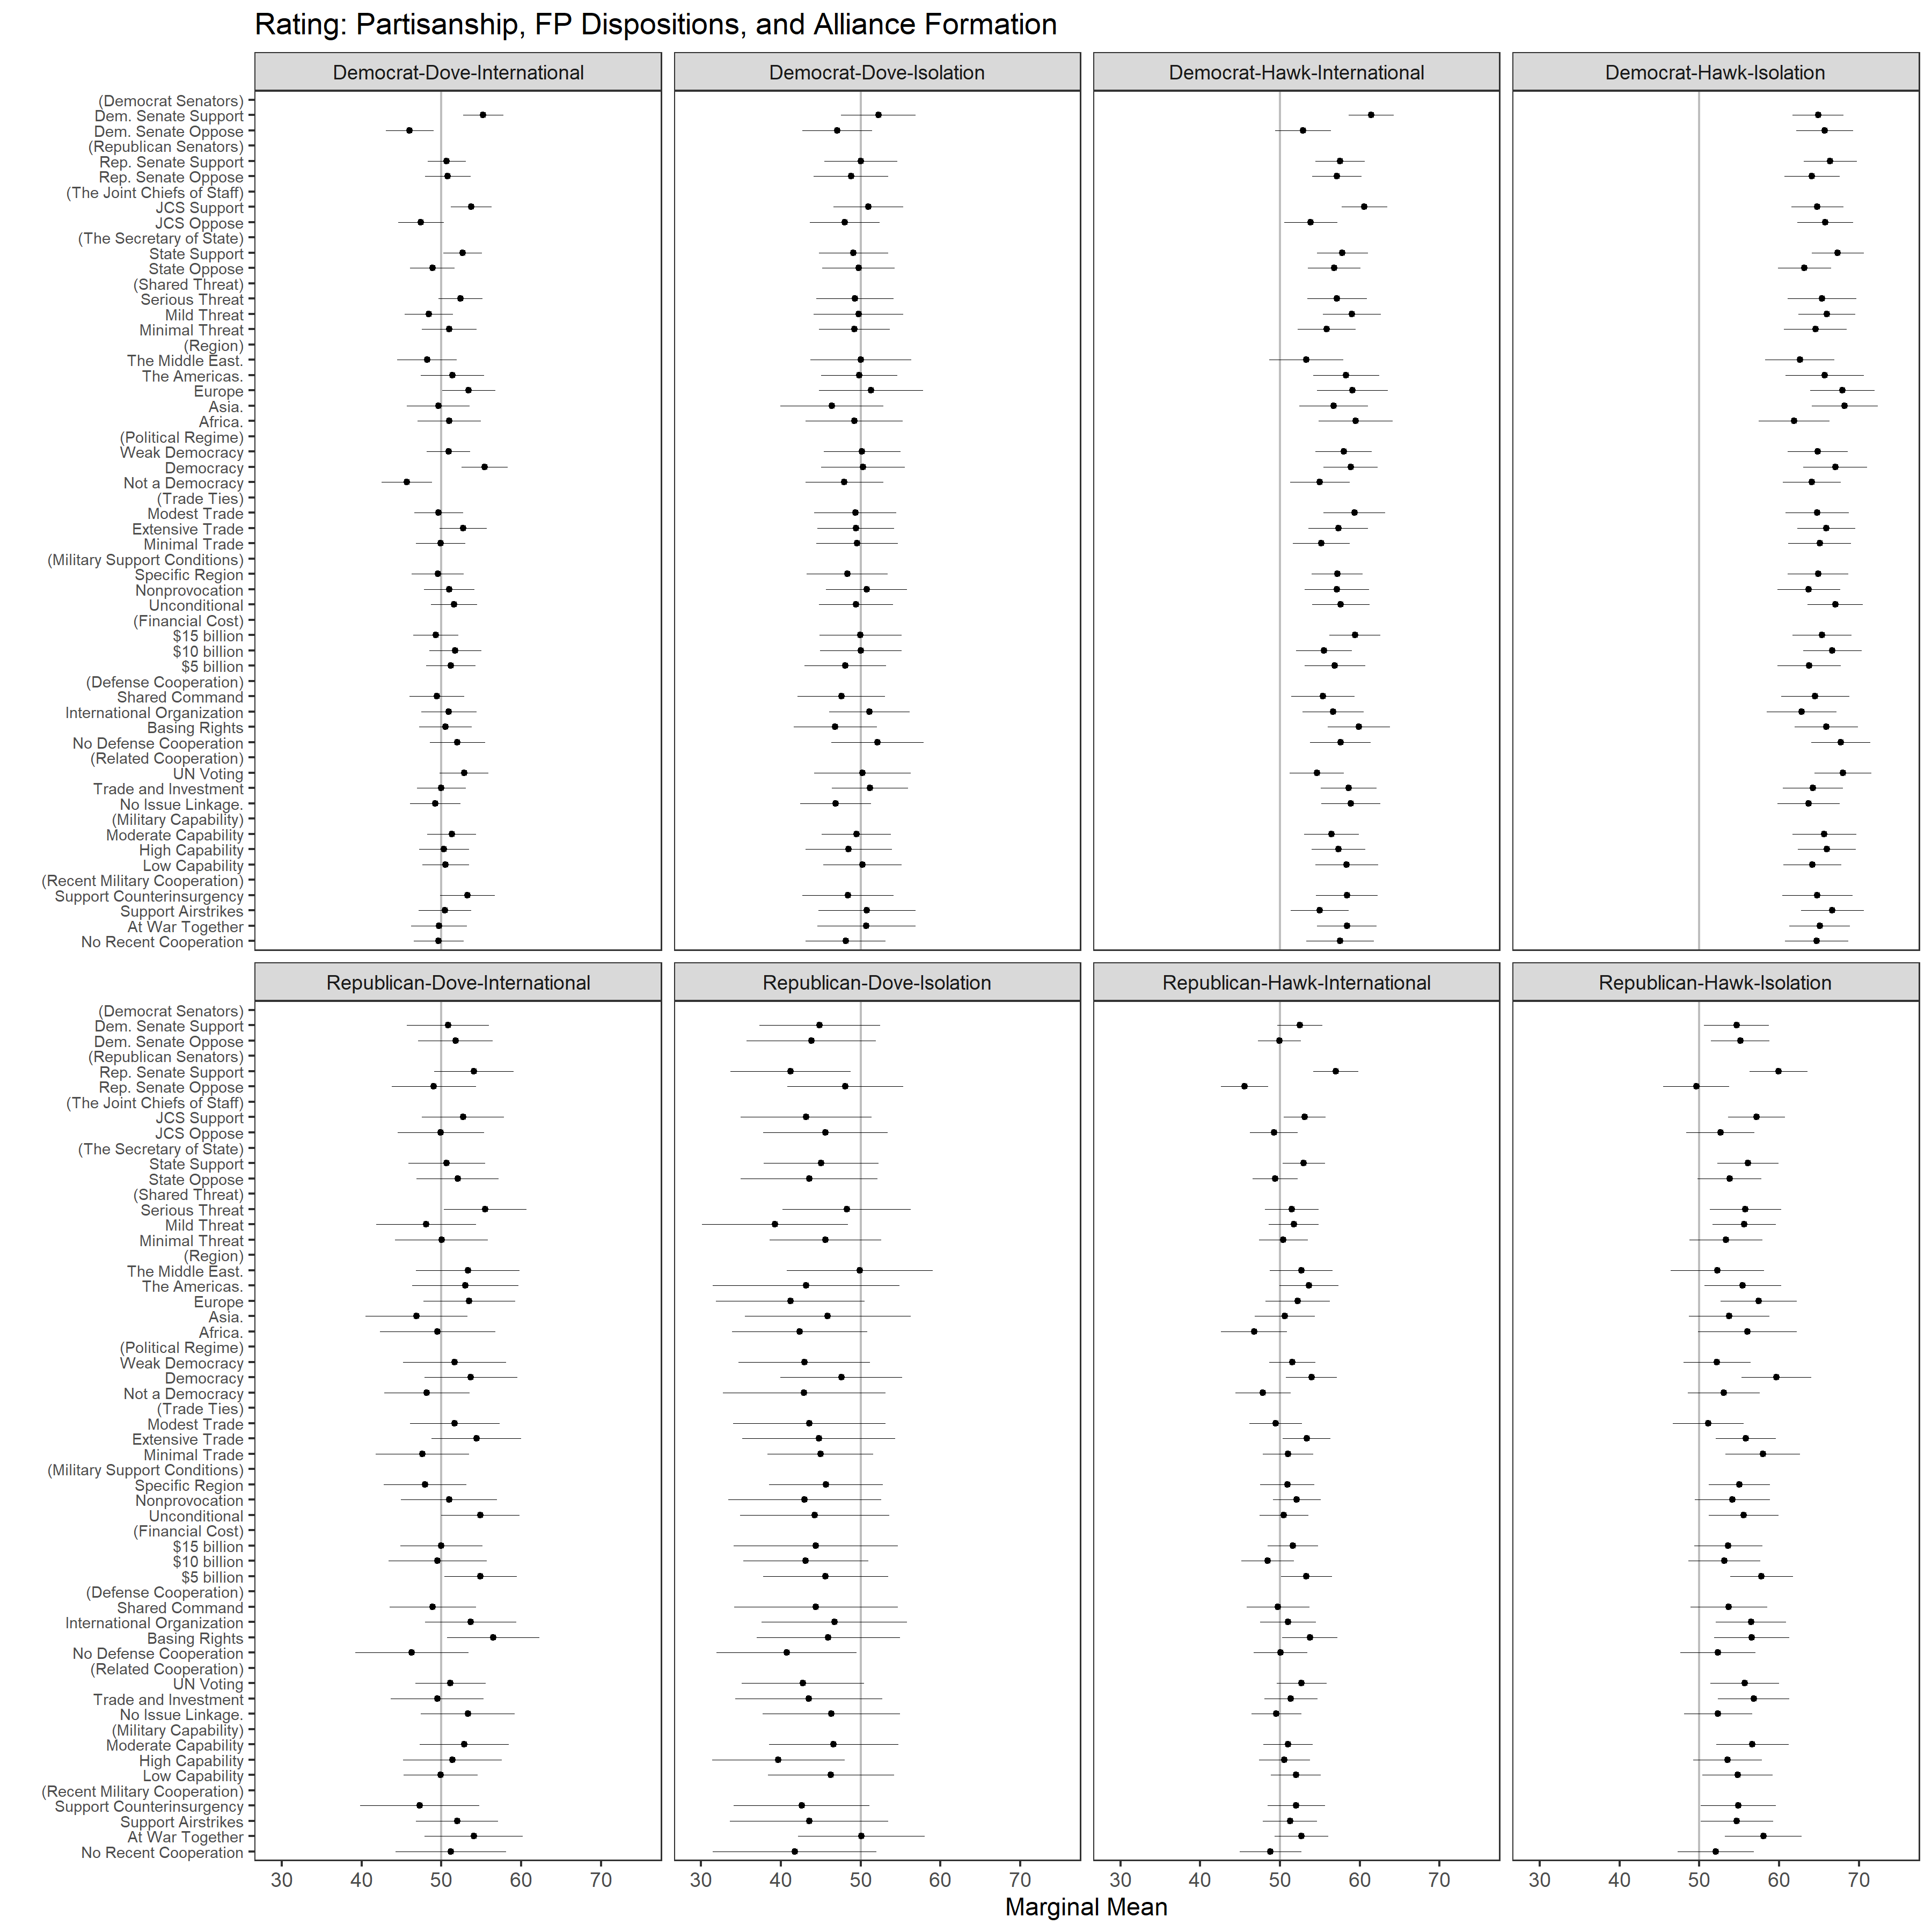
\includegraphics[width=0.95\textwidth]{party-dispo-formapp.png}
	\caption{Marginal means of ratings for hypothetical new alliances based on elite cues across party identification and foreign policy dispositions. For each group, the estimates mark the marginal mean of support for alliance participation under different alliance treatments. Components marked with abbreviated labels and alliance characteristics omitted to make the plot more legible. Independents omitted.}
	\label{fig:party-dispo-form}
\end{figure}


While foreign policy dispositions clearly impact alliance ratings, there are also partisan differences that match those in the manuscript. 
Hawkish and dovish Republicans have the lowest alliance ratings. 
Hawkish and isolationist Democrats express high ratings of alliances in general.  
Last, hawkish Republicans and internationalist Democrats are most responsive to elite cues. 


\begin{figure}[htpb]
	\centering
		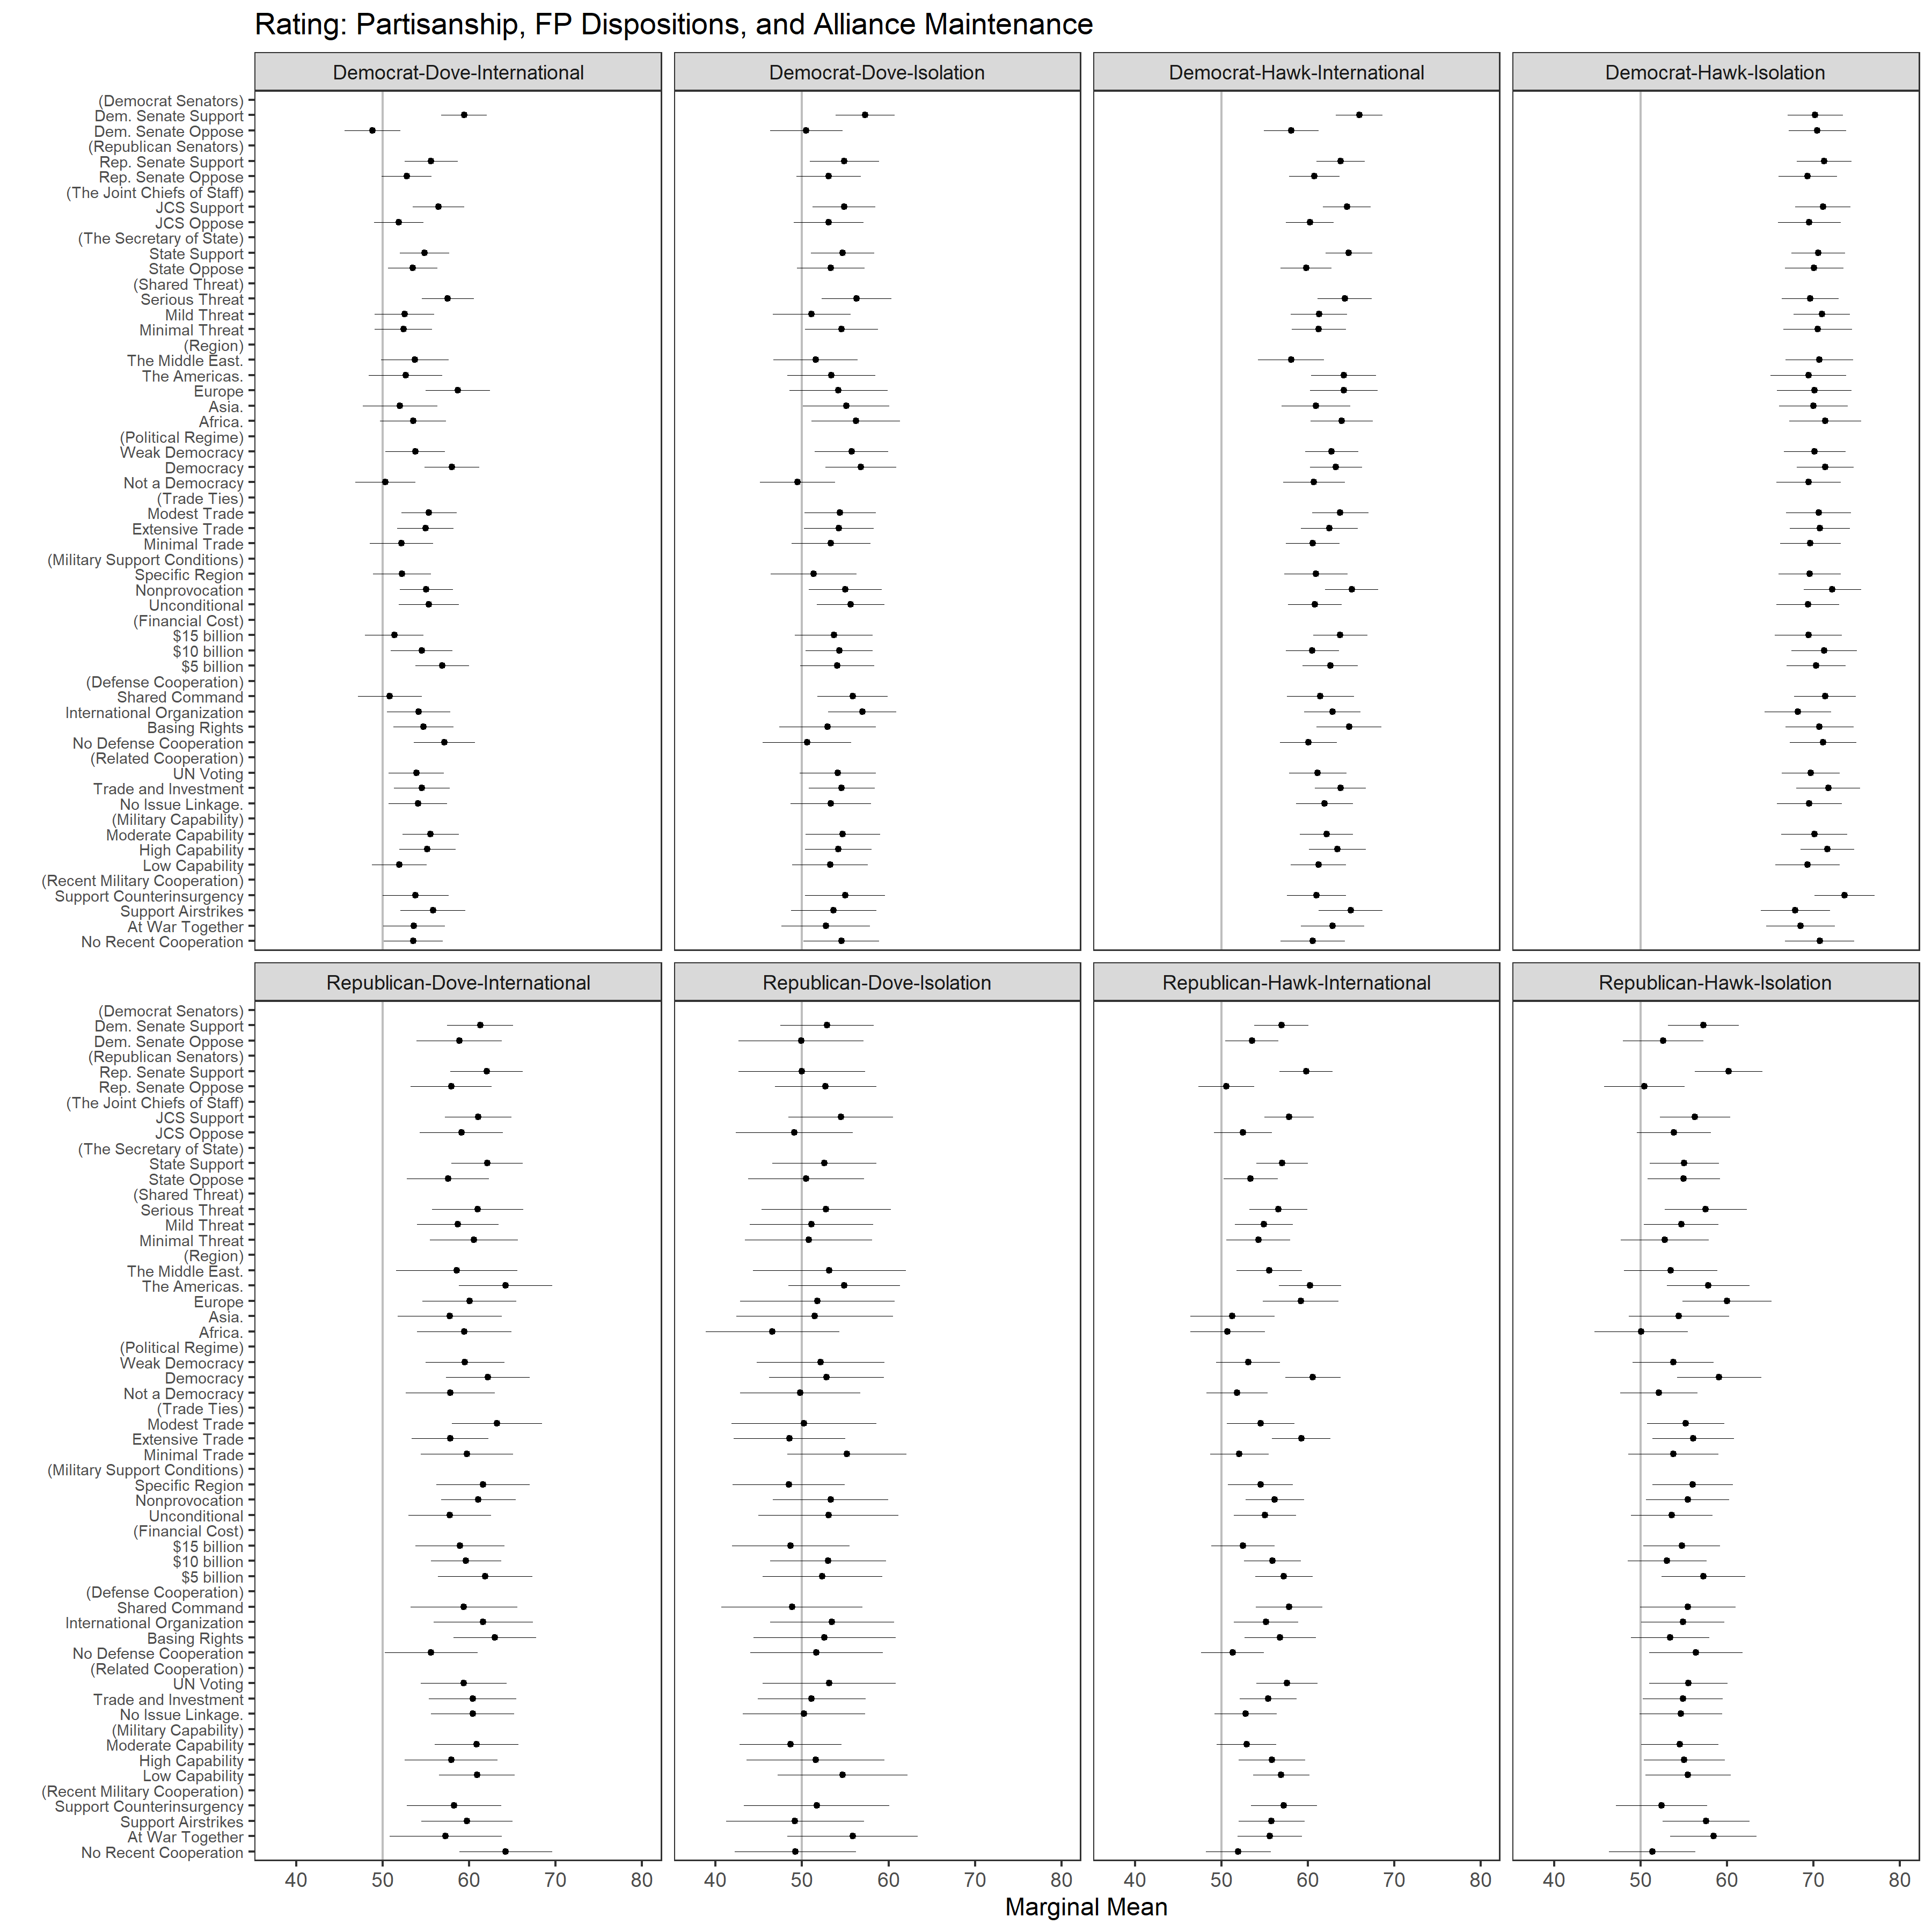
\includegraphics[width=0.95\textwidth]{party-dispo-mainapp.png}
	\caption{Marginal means of ratings for hypothetical existing alliances across party identification and foreign policy dispositions. For each group, the estimates mark the marginal mean of support for alliance participation under different alliance treatments. Components marked with abbreviated labels and alliance characteristics omitted to make the plot more legible. Independents omitted.}
	\label{fig:party-dispo-main}
\end{figure}


\newpage 


% intended this for the initial competing frame- doesn't really help with the subgroup analyses, however.
%\section{Alternative Alliance Profile Distributions}
%
%
%\citet{delaCuestaetal2021} observe that the distribution of profiles can affect inferences, especially when assuming a uniform distribution of profiles.
%Although using a uniform randomization scheme ensures sufficient variation in elite cues and presents a wide variety of alliance profiles, some profiles may be more likely than others. 
%To investigate how alternative profile distributions affect the AMCE estimates, I implemented the model based exploratory analysis recommendations of \citet{delaCuestaetal2021}. 
%
%
%The exploratory analysis requires alternative assumptions about the marginal distributions of the alliance attributes.
%\autoref{tab:conjoint-vars-margins} summarizes the assumed marginal distributions for the alliance formation experiment. 
%I used data from the ATOP project \citep{Leedsetal2002} to measure the frequency of different alliance treaty obligations. 
%I then make alternative assumptions about elite cues, starting with less consistent support from Republican Senators, relative to Democratic Senators, military leaders and diplomats. 
%I then use the observed distribution of U.S. trade ties, the distribution of allied military capability and U.S. ally democracy to approximate the population frequency of these attributes. 
%I also assume that serious common threats are unusual. 
%Data on recent military cooperation is based on the size of the coalition of the willing in Iraq as a share of states in the international system. 
%The assumed population distribution of financial costs assumes that most alliances are relatively inexpensive, but a few have substantial costs. 
%
%
%
%\begin{table}
%\begin{adjustbox}{width = .99\textwidth}
%\begin{tabular}{lc} 
%\hline \\ 
%\textbf{Attributes} & \textbf{Values} \\
%\hline \\ 
%Republican Senators & Support an alliance with this country. \textbf{.6} \\
%                    & Oppose an alliance with this country. \textbf{.4} \\ 
%                    
%Democratic Senators & Support an alliance with this country. \textbf{.8} \\
%                    & Oppose an alliance with this country. \textbf{.2}\\ 
%                    
%The Joint Chiefs of Staff & Support an alliance with this country. \textbf{.9}\\
%                    & Oppose an alliance with this country.\textbf{.1}  \\ 
%                    
%The Secretary of State & Supports an alliance with this country. \textbf{.9} \\
%                    & Opposes an alliance with this country. \textbf{.1} \\ 
%% data from: https://www.census.gov/foreign-trade/Press-Release/2019pr/12/exh4s.pdf                    
%Trade Ties          & The United States has minimal trade ties with this country. \textbf{.5} \\
%                    & The United States has modest trade ties with this country. \textbf{.25}\\
%                    & The United states has extensive trade ties with this country. \textbf{.25} \\ 
%% modified from Tomz and Weeks 2013 APSR: https://web.stanford.edu/~tomz/pubs/TomzWeeks-2013-11-Appendix.pdf 
%Partner Political Regime    & This country is not a democracy, and shows no sign of becoming a democracy. \textbf{.2}\\
%                    & This country is a democracy, but shows signs that it may not remain a democracy. \textbf{.1} \\ % democ backsliding
%                    & This country is a democracy, and shows every sign that it will remain a democracy. \textbf{.7}\\
%                    
%Partner Military Capability & 10,000 soldiers and spends 1\% of their GDP on the military. \textbf{.75}\\ % low
%                    & 80,000 soldiers and spends 2\% of their GDP on the military. \textbf{.2} \\ % moderate
%                    & 250,000 soldiers and spends 3\% of their GDP on the military. \textbf{.05}\\ % high 
%                    
%Shared Threat       & The United States and this country face minimal common threats. \textbf{.5} \\ 
%                    & The United States and this country face modest common threats. \textbf{.35} \\
%                    & The United States and this country face serious common threats. \textbf{.15} \\
%% data from https://en.wikipedia.org/wiki/Multi-National_Force_%E2%80%93_Iraq                
%Recent Military Cooperation  & This country has not participated in recent U.S. military operations. \textbf{.46} \\ 
%                    & This country recently supported U.S. airstrikes against terrorists. \textbf{.18}\\
%                    & This country recently supported U.S. counterinsurgency operations. \textbf{.18}\\
%                    & This country recently fought with the United States in a war. \textbf{.18}\\
%                    
%Financial Cost      & This alliance requires \$5 billion in annual U.S. defense spending.  \textbf{.6}\\ 
%                    & This alliance requires \$10 billion in annual U.S. defense spending.  \textbf{.3}\\ 
%                    & This alliance requires \$15 billion in annual U.S. defense spending.  \textbf{.1}\\ 
%                    
%Conditions on Support  & The alliance treaty promises military support in any conflict. \textbf{.5} \\ 
%                    & The alliance treaty promises military support only if this country is attacked. \textbf{.25} \\ 
%                    & The alliance treaty promises military support only if the conflict takes place in this country's region. \textbf{.25} \\
%                    
%Defense Cooperation & None. \textbf{.56} \\ 
%                    & The alliance treaty provides basing rights for U.S. troops. \textbf{.21}\\
%                    & The alliance treaty includes a shared military command. \textbf{.07} \\
%                    & The alliance treaty includes an international organization to coordinate defense policies. \textbf{.17} \\ 
%% Issue linkages                    
%Related Cooperation & None. \textbf{.86} \\
%                    & The alliance is linked to greater trade and investment with the United States. \textbf{.07}\\ 
%                    & The alliance is linked to greater support for the United States in the United Nations. \textbf{.07} \\ 
%                    
%Region              & Europe. \textbf{.4}\\ 
%                    & Africa. \textbf{.03}\\
%                    & The Middle East. \textbf{.07}\\ 
%                    & Asia.\textbf{.1} \\   
%                    & The Americas. \textbf{.4}\\ 
%                                                                            
%\hline \\
%\end{tabular}
%\end{adjustbox}
%\caption{Table of alliance attributes in conjoint experiment profiles with alternative frequency assumptions. Frequencies for model-based population average marginal component effect estimation in bold. I use the same set of attributes as treatments in the alliance formation and maintenance experiments.} 
%\label{tab:conjoint-vars-margins}
%\end{table}
%
%
%I use the marginal distribution of alliance attributes in \autoref{tab:conjoint-vars-margins} as the target distribution for the alliance formation experiment, but use a different procedure for the maintenance experiment. 
%Rather than use an assumed distribution, I check the maintenance results using data from observed U.S. alliances as the target distribution. 
%In this analysis, I use data from U.S. alliance partners in 2018 to measure the prevalence of democracy, trade ties, military capability, threat and treaty obligations. 
%
%
%The population AMCE analysis has important disadvantages. 
%I cannot undertake subgroup analyses of partisanship and foreign policy dispositions, which are at the heart of the analysis. 
%Furthermore, I must omit the region attribute in the observed data estimates of the alliance maintenance AMCES, given the lack of U.S. alliances in Africa. 
%I also have to select conditions on military support or defense cooperation values in alliances with more than one value for these attributes. 
%For example, NATO has basing rights and an international organization, and I select basing rights as that commitment is more consequential.  
%Establishing the population of elite cues also required some assumptions about which alliances military and diplomatic elites would likely oppose.
%While Democrat and Republican Senators have expressed skepticism of some U.S. alliances, military and diplomatic elites are usually more reticent, but some cases with opposition are necessary for analysis. 
%
%
%% quick overview of results 
%\autoref{fig:pop-amce-main} and \autoref{fig:pop-amce-form} plot the population AMCE estimates, relative to the sample AMCEs reported in the manuscript. 
%Even under alternative distributional assumptions, elite cues, allied democracy and financial costs exert substantial influence on alliance attitudes. 
%The population AMCE estimates have much higher uncertainty, so some are not statistically significant at conventional levels, despite estimates in the same direction with greater magnitude. 
%This likely reflects reduced variation in elite cues. 
%The lack of differences in different AMCE levels for attributes with more than two levels is also a concern. 
%
%
%
%\begin{figure}
%	\centering
%		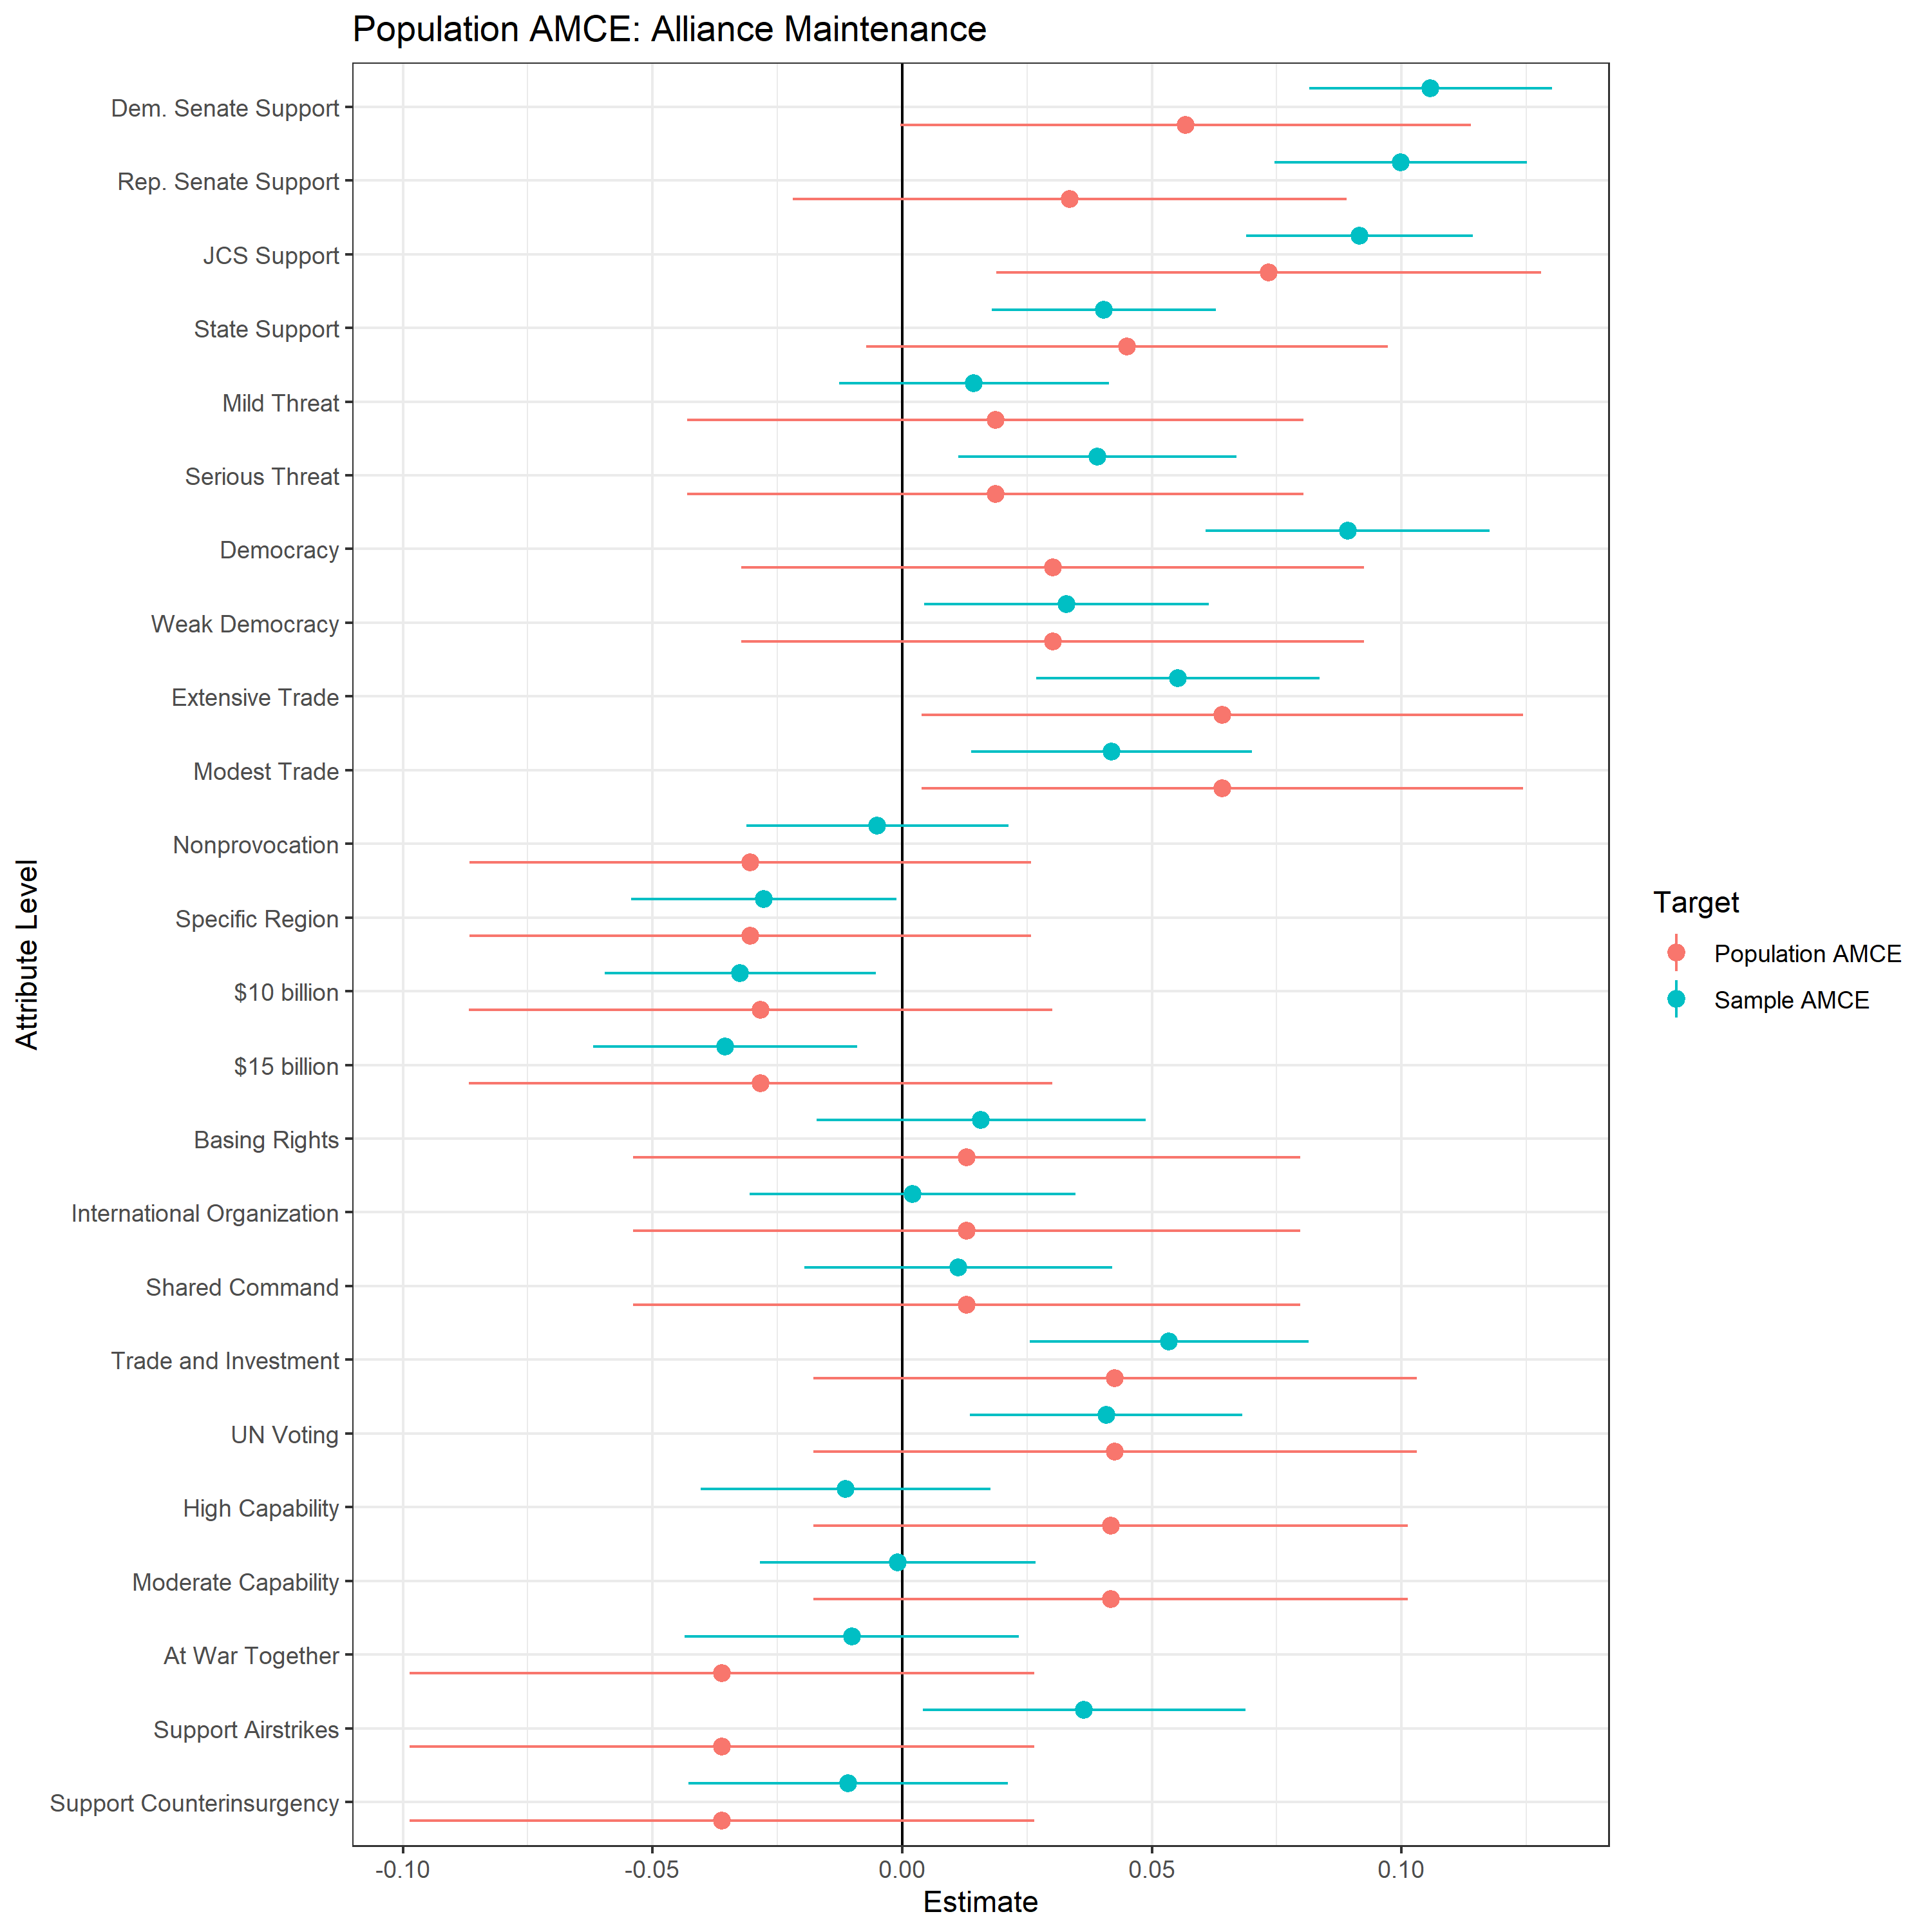
\includegraphics[width=0.95\textwidth]{pop-amce-main.png}
%	\caption{Estimated AMCE of difference alliance attributes on support for alliance maintenance under alternative distributional assumptions. In this model-based exploratory analysis, the population distribution is based on observed U.S. alliances.}
%	\label{fig:pop-amce-main}
%\end{figure}
%
%
%\begin{figure}
%	\centering
%		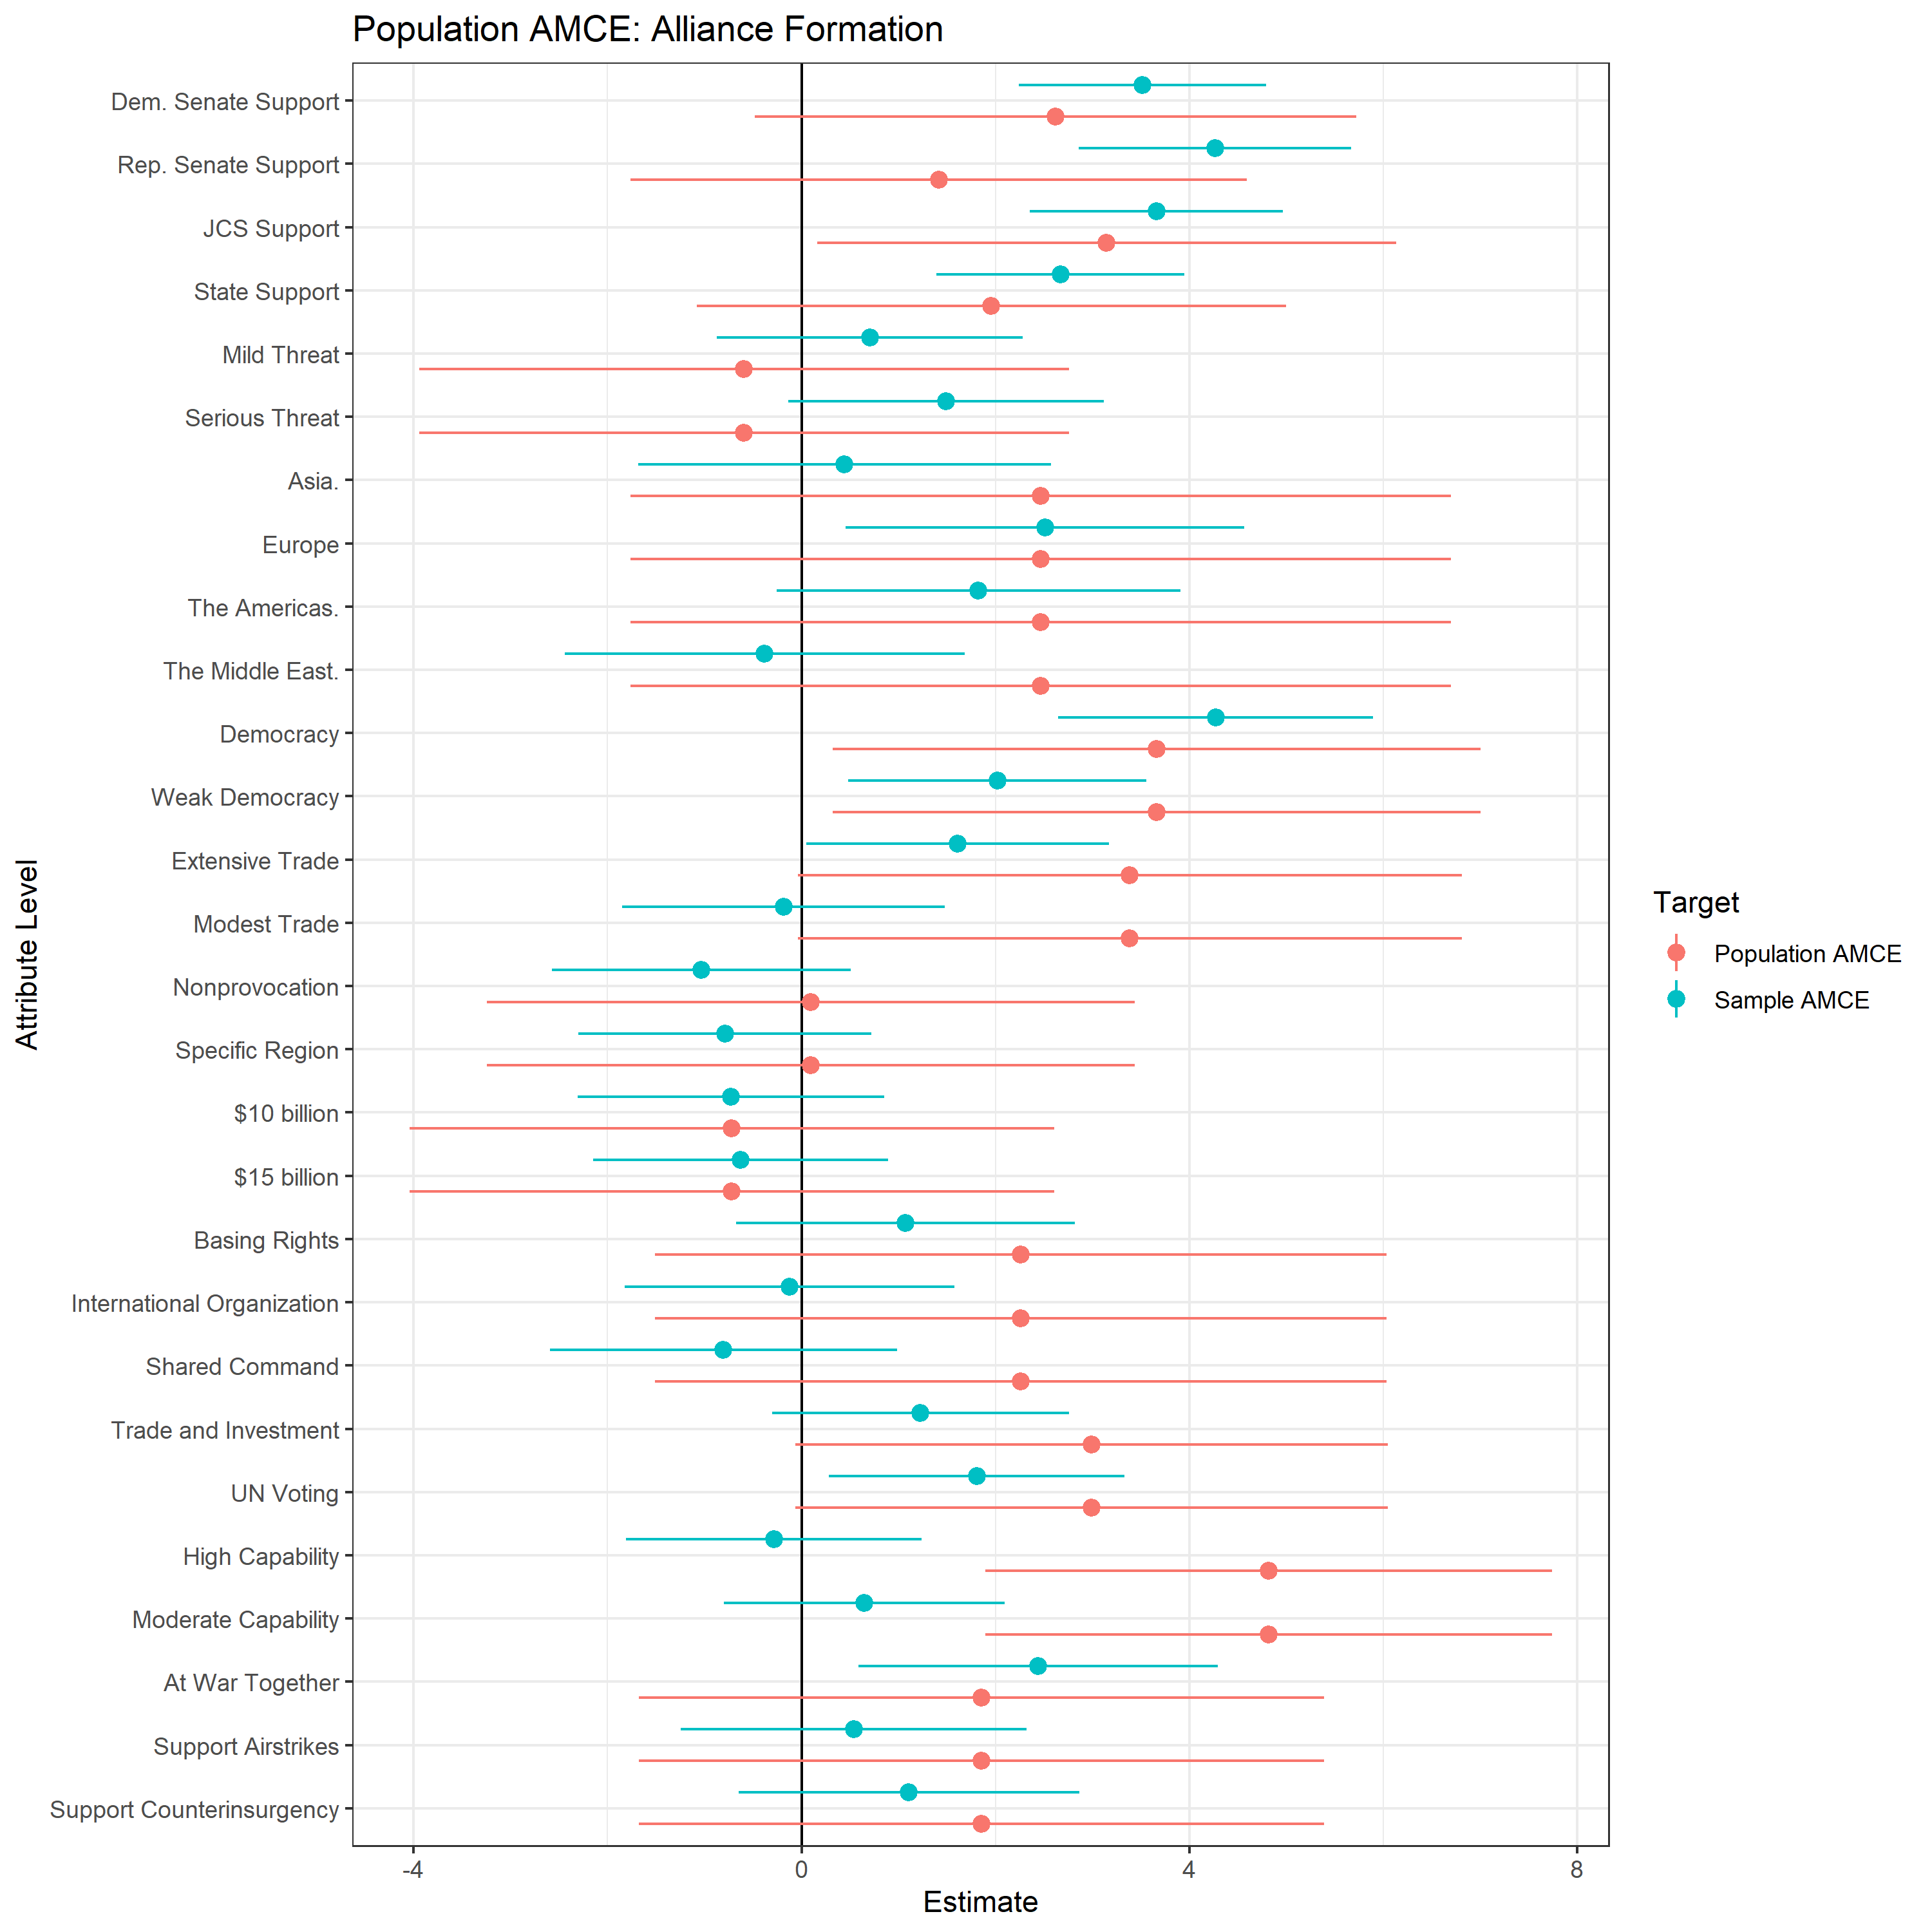
\includegraphics[width=0.95\textwidth]{pop-amce-form.png}
%	\caption{Estimated AMCE of difference alliance attributes on support for alliance formation under alternative distributional assumptions. In this model-based exploratory analysis, the population distribution is based on a mix of all alliances and observed U.S. alliances.}
%	\label{fig:pop-amce-form}
%\end{figure}
%
%% summarize differences
%There are also some differences between the population and sample AMCE estimates. 
%Trade exerts a stronger influence on alliance attitudes under different marginal attribute distributions of the attributes. 
%In the alliance formation experiment, elite cues are less influential than allied democracy, trade and capability. 
%How these differences would alter the conclusion of the subgroup analysis is unclear, however. 
%
%


\section{Distribution of Foreign Policy Dispositions by Party}

In this section, I show the number of respondents in each group of partisans and foreign policy dispositions, as well as the strength of their partisan affiliations.
\autoref{tab:party-dispo-main} summarizes these values for the alliance maintenance experiment. 
\autoref{tab:party-dispo-form} contains the same information for the alliance formation experiment. 


\begin{table}[htbp]
\centering
\begin{tabular}{lc}
  \hline
 Disposition  & Number of Respondents \\ 
  \hline
Republican-Dove-International &  69 \\ 
  Independent-Dove-International &  82 \\ 
  Democrat-Dove-International & 240 \\ 
  \hline
  Republican-Hawk-International & 236 \\ 
  Independent-Hawk-International &  71 \\ 
  Democrat-Hawk-International & 242 \\
  \hline  
  Republican-Dove-Isolation &  53 \\ 
  Independent-Dove-Isolation &  46 \\ 
  Democrat-Dove-Isolation & 134 \\ 
  \hline
  Republican-Hawk-Isolation & 180 \\ 
  Independent-Hawk-Isolation &  34 \\ 
  Democrat-Hawk-Isolation & 194 \\ 
   \hline
\end{tabular}
\caption{Number of respondents in each group of partisanship and foreign policy disposition for the alliance maintenance experiment.} 
\label{tab:party-dispo-main}
\end{table}


\begin{table}[htbp]
\centering
\begin{tabular}{lc}
  \hline
 Disposition  & Number of Respondents \\ 
  \hline
Republican-Dove-International &  81 \\ 
  Independent-Dove-International &  65 \\ 
  Democrat-Dove-International & 232 \\ 
  \hline
  Republican-Hawk-International & 268 \\ 
  Independent-Hawk-International &  76 \\ 
  Democrat-Hawk-International & 223 \\ 
  \hline
  Republican-Dove-Isolation &  47 \\ 
  Independent-Dove-Isolation &  43 \\ 
  Democrat-Dove-Isolation & 120 \\ 
  \hline
  Republican-Hawk-Isolation & 190 \\ 
  Independent-Hawk-Isolation &  48 \\ 
  Democrat-Hawk-Isolation & 213 \\ 
   \hline
\end{tabular}
\caption{Number of respondents in each group of partisanship 
               and foreign policy disposition for the alliance formation experiment.} 
\label{tab:party-dispo-form}
\end{table}


The distribution of foreign policy dispositions by partisan affiliation is similar across the two experiments. 
Most Republicans are hawkish, with a slight preponderance of militant internationalists. 
Democrats have an internationalist bent and are more equally split between hawks and doves. 
The few independents lean towards internationalism, but have a more even distribution of foreign policy dispositions. 


This categorical breakdown uses numeric questions on militant assertiveness and isolationism to divide respondents. 
\autoref{fig:dispo-part-plots} summarizes the full distribution of these variables by party. 
For the categorical measures, isolationists scored a 4 or 5 on that scale, while hawks had a militant assertiveness score of three or greater. 
In both experiments and parties, isolationism is concentrated at moderate values of militant assertiveness just above the midpoint of that scale, so many hawks express some isolationist tendencies as well.    


\begin{figure}
	\centering
		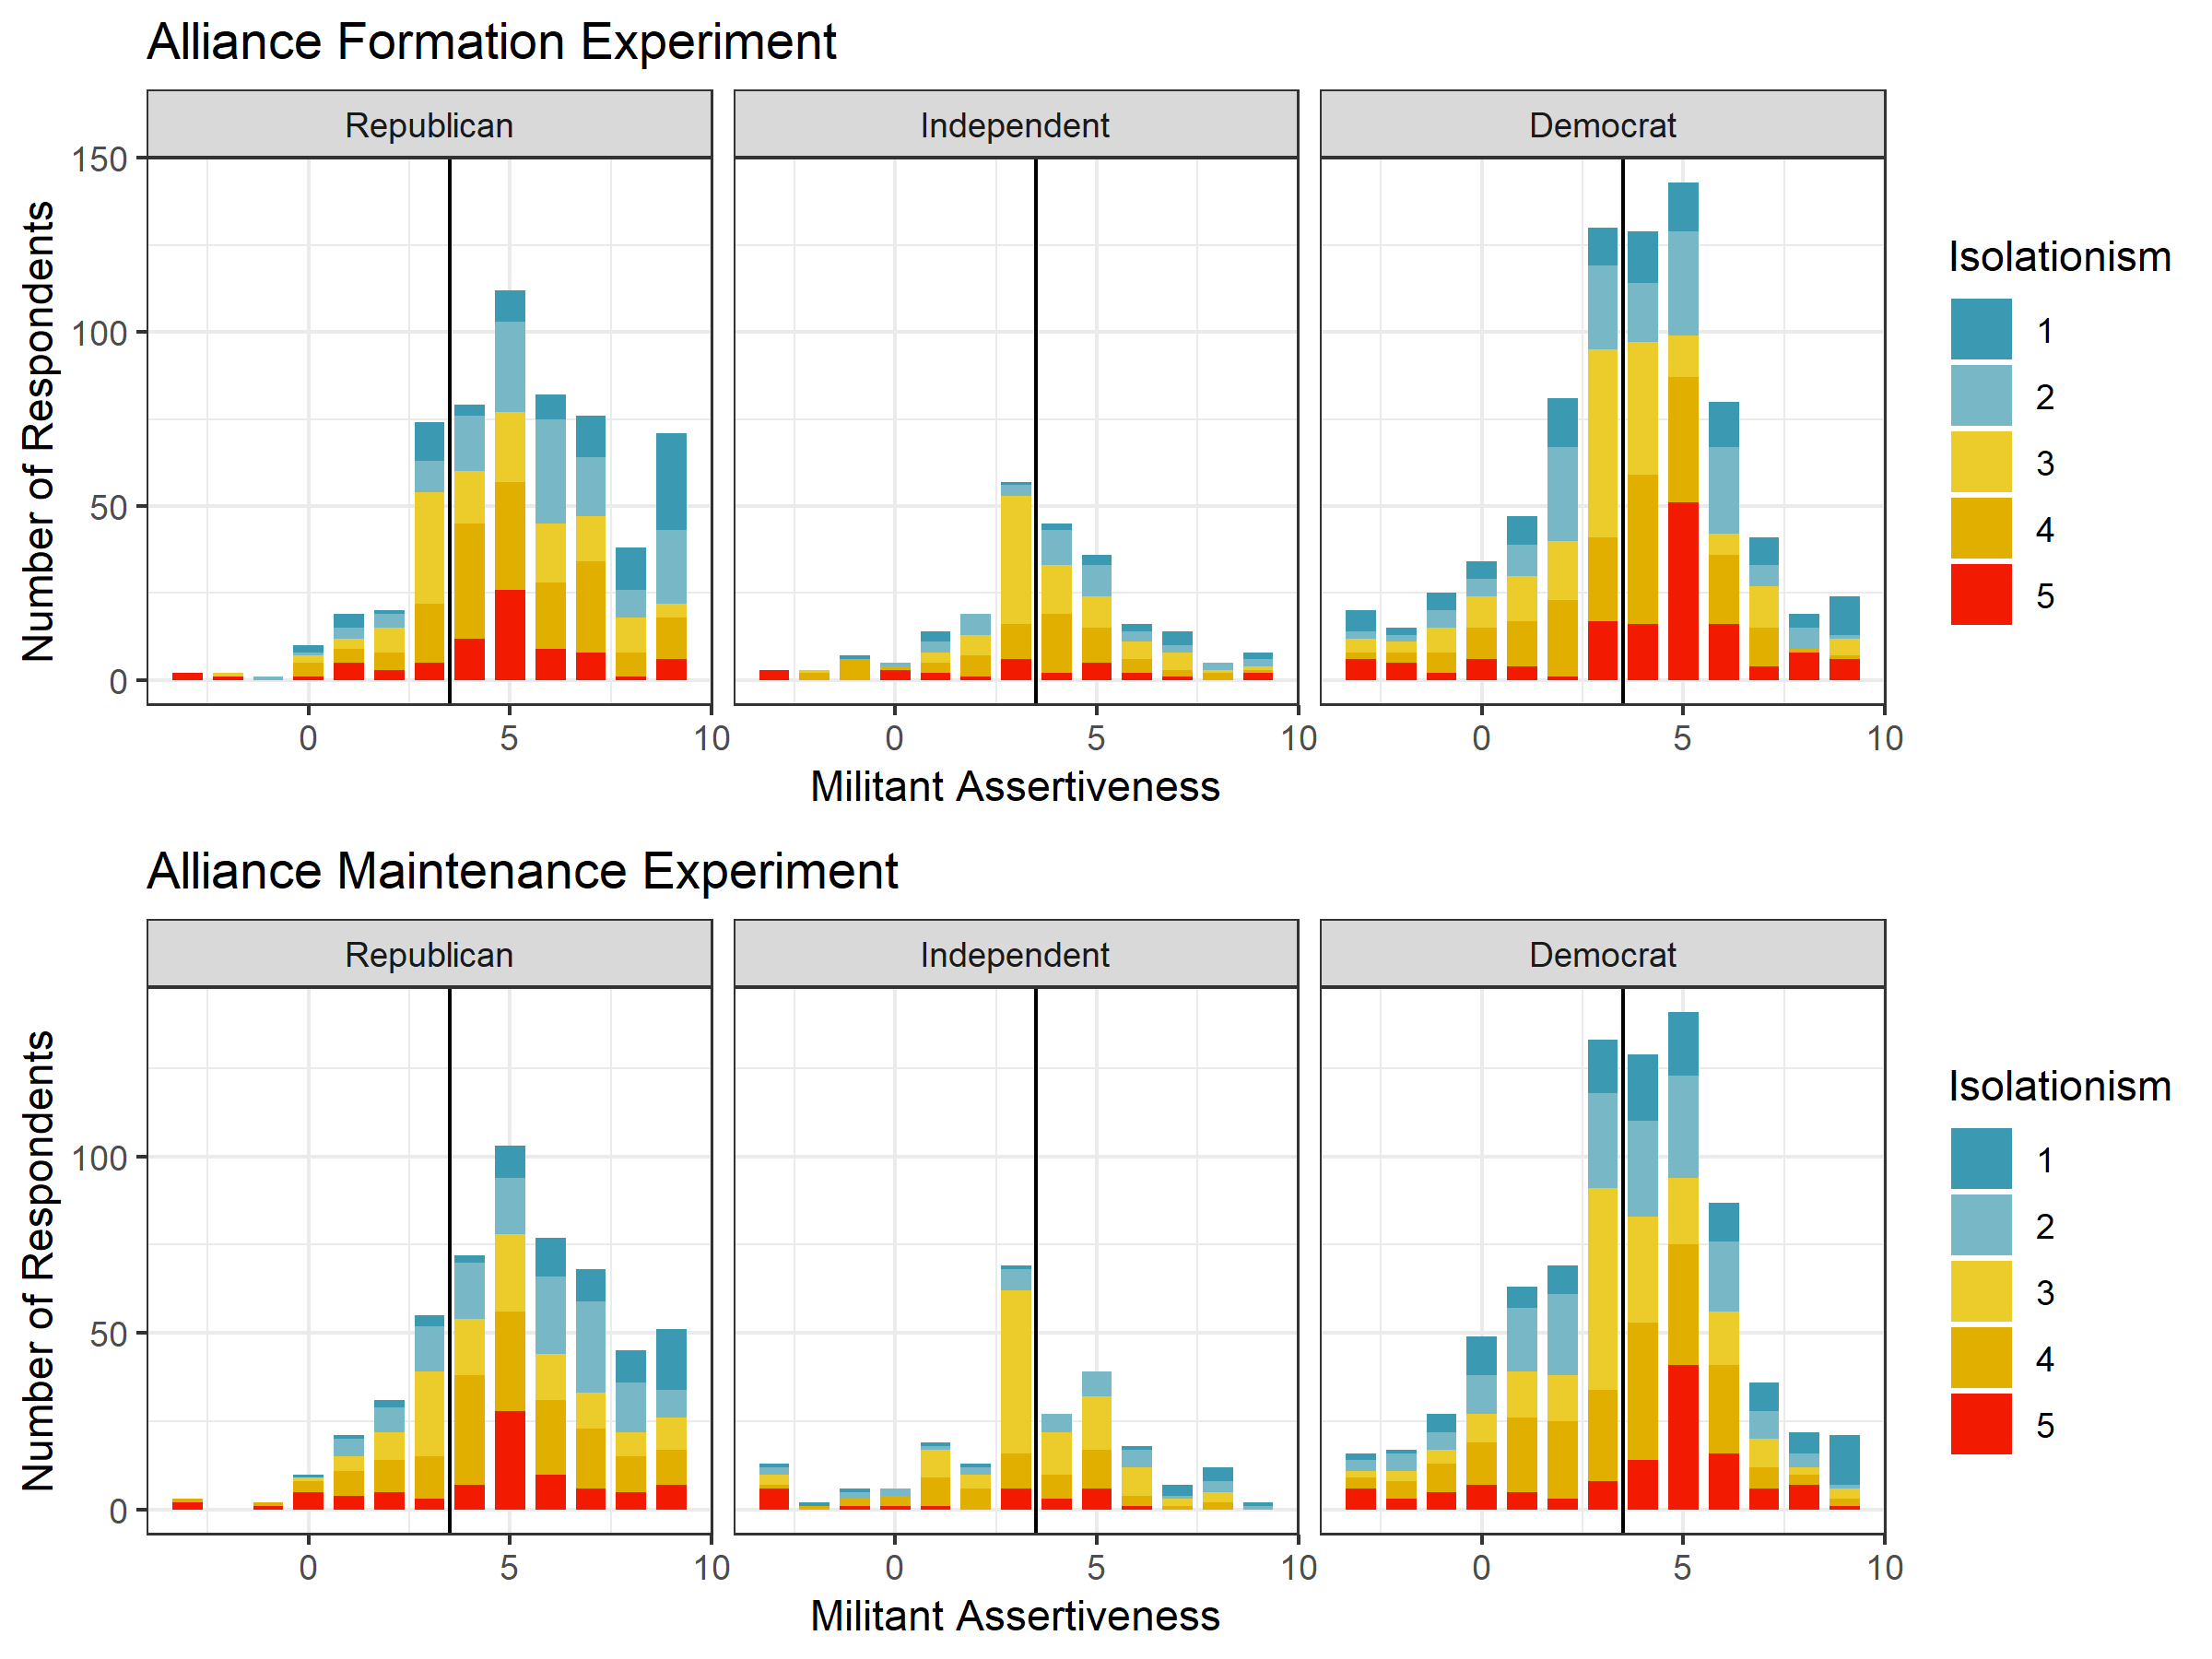
\includegraphics[width=0.95\textwidth]{dispo-part-plots.png}
	\caption{Bar chart of militant assertiveness and isolationism by partisan affiliation. Colors within each bar divide respondents at each level of militant assertiveness by isolationism. The vertical line marks the cut point for the categorical distinction between hawks and doves at the midpoint of the militant assertiveness scale.}
	\label{fig:dispo-part-plots}
\end{figure}



The in vs out group dynamics between party wings imply that some wings may be less attached to their party. 
To assess this, I scored partisan attachment by giving individuals who described themselves as ``other Republicans,'' with a value of one, individuals who ``lean Republican'' with a two, and ``strong Republicans'' with three.
\autoref{fig:part-str-plots} presents the average partisan strength for each of the four foreign policy dispositions in the experiment.


\begin{figure}
	\centering
		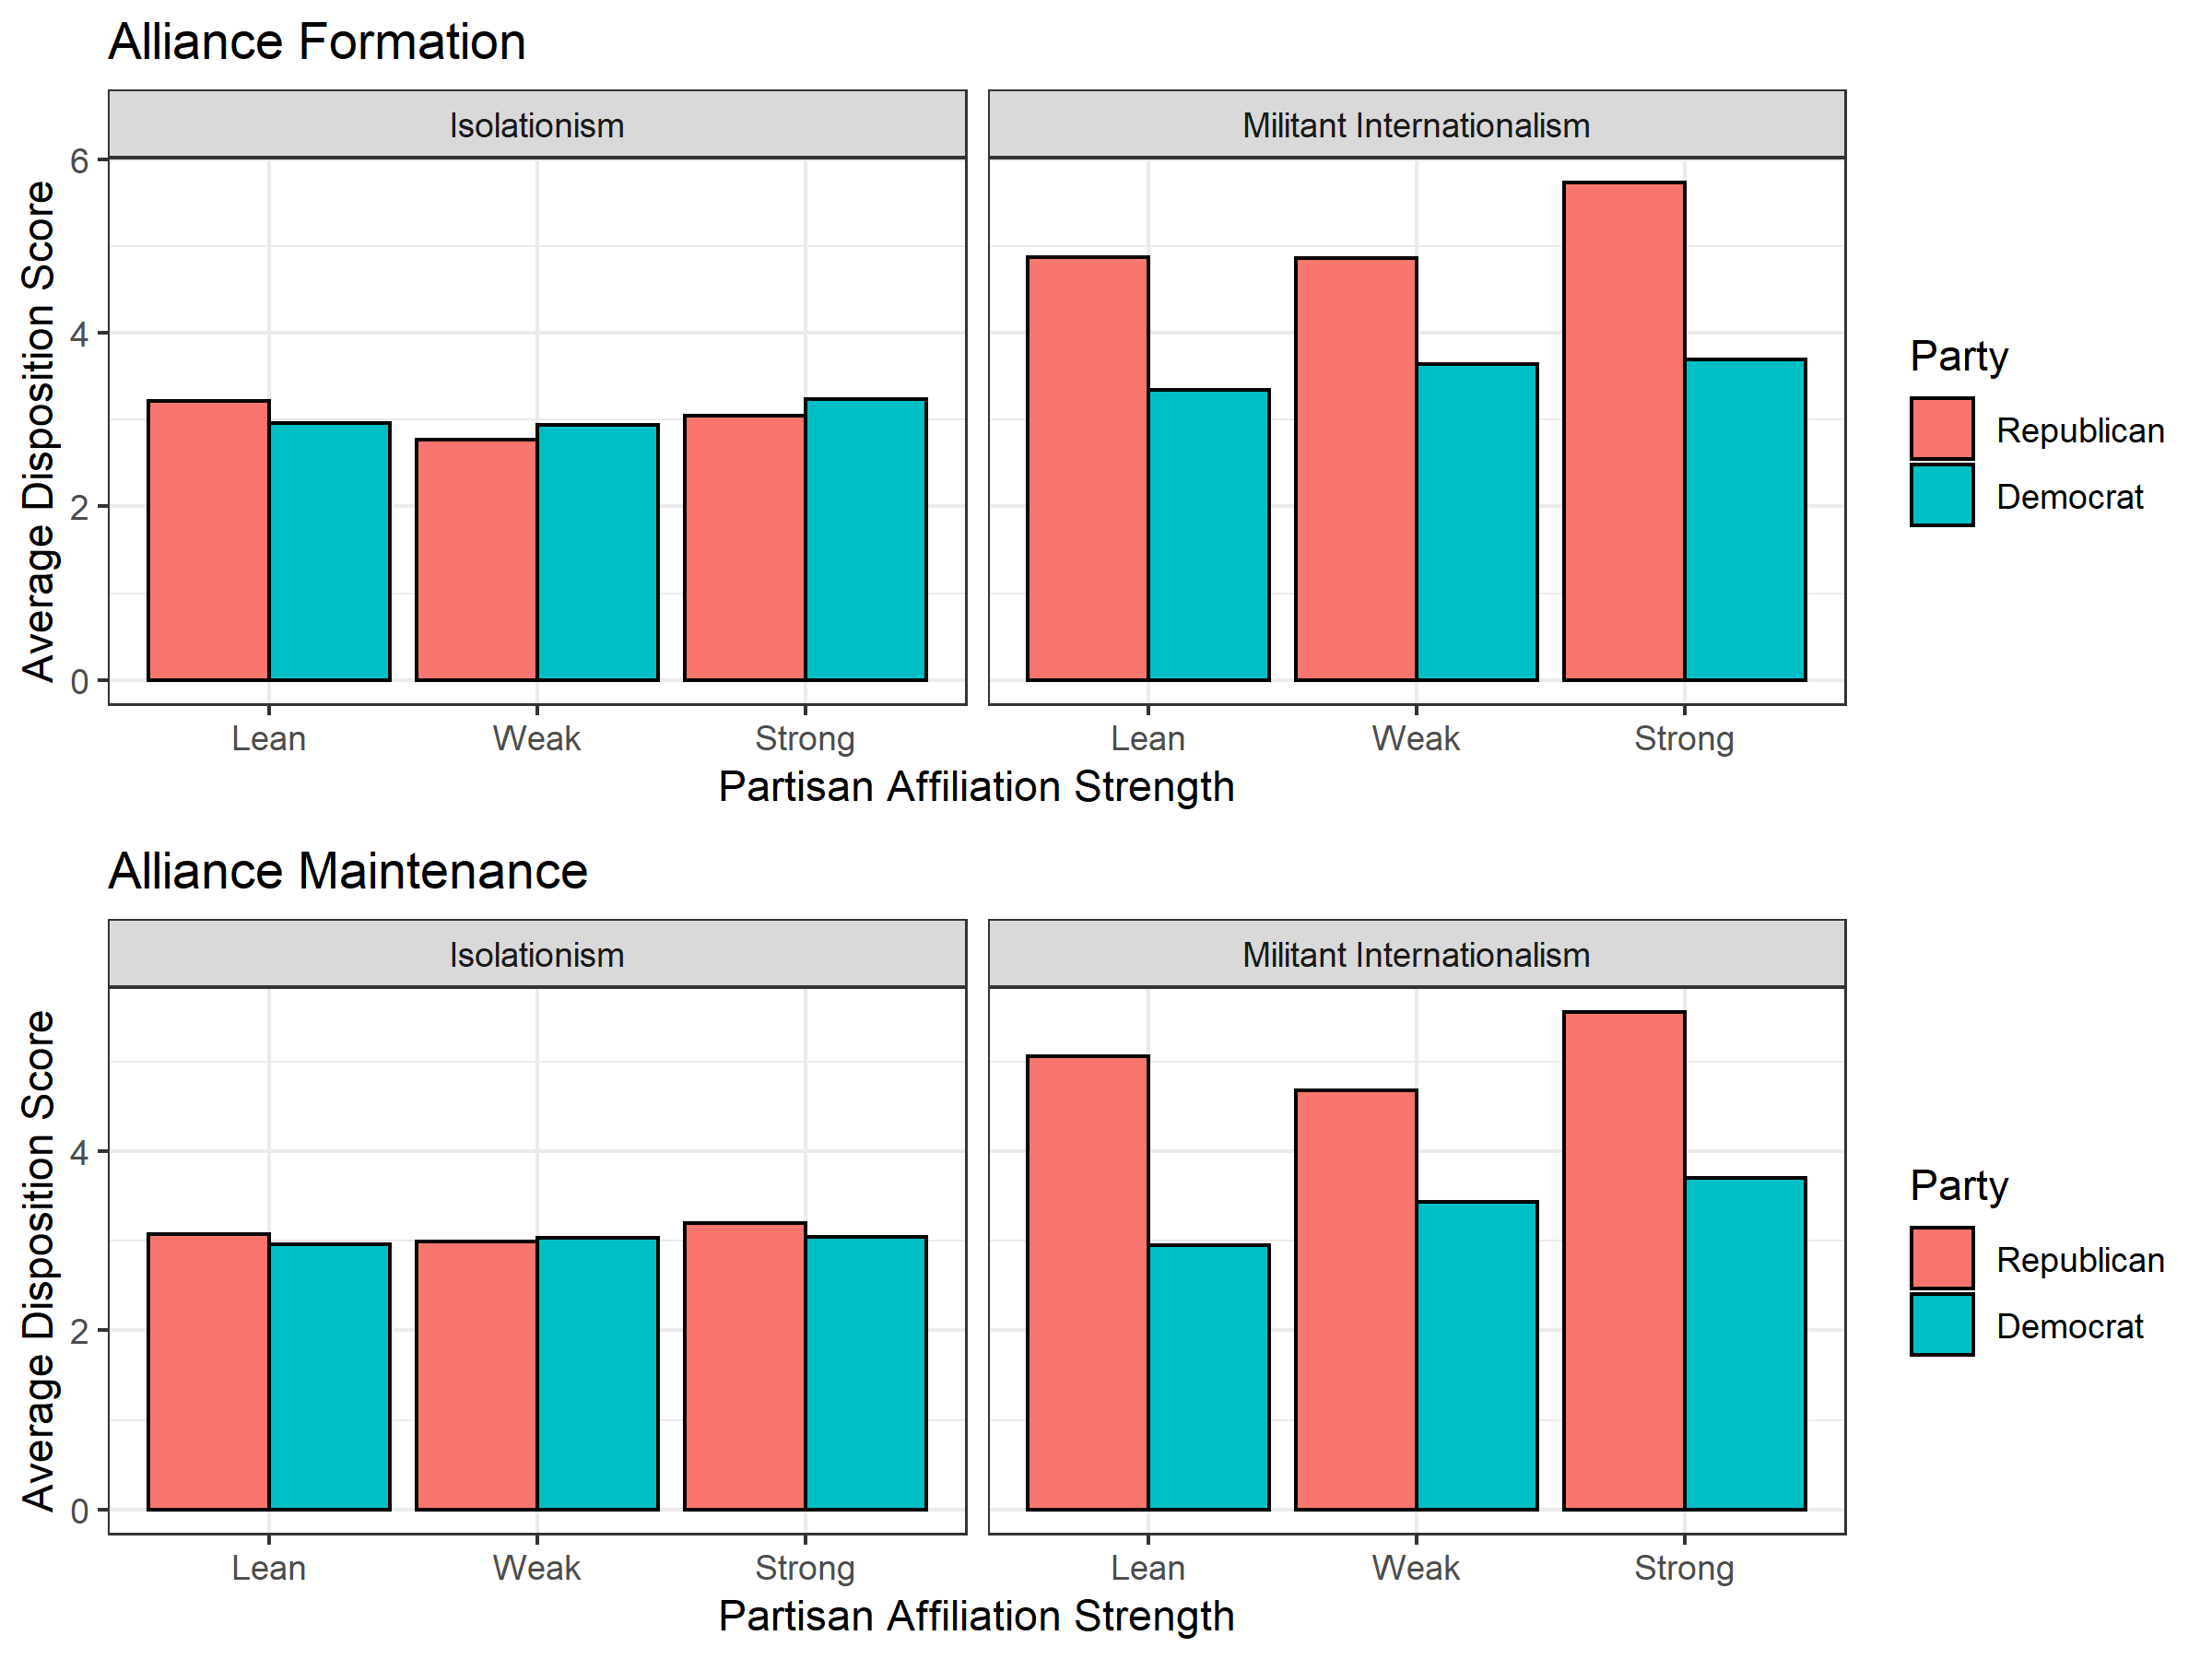
\includegraphics[width=0.95\textwidth]{part-str-plots.png}
	\caption{Bar chart of partisan affiliation strength across foreign policy dispositions. Colors distinguish between the alliance formation and maintenance experiments. The error bars mark 95\% confidence interval of average partisan attachment.}
	\label{fig:part-str-plots}
\end{figure}


I find little difference in partisan attachment across the different foreign policy dispositions.
Dovish Republicans are somewhat less attached to their party, but there is also more variation in attachment within this small subset of respondents. 
The difference in mean partisan attachment between hawkish and internationalist Republicans and their co-partisan hawkish isolationists in the alliance formation experiment is .12. 
This is one of the two largest gaps in either sample. 
Therefore, individuals in different wings of the party are not necessarily less attached to the party itself.

 
Perhaps individuals with rigid alliance attitudes differ not in partisan attachment, but in their political participation.\footnote{Thanks to an anonymous reviewer for raising this point.}
To assess this point, I use education as a proxy for political engagement.
I find inconsistent differences in educational attainment across the different foreign policy dispositions, however.
\autoref{fig:part-educ-plots} shows these results.
Dovish and internationalist Republicans have the lowest average education of any subgroup. 
Hawkish isolationist Democrats with rigid alliance attitudes have the highest educational attainment. 
Republican doves with isolationist views have typical education levels, relative to the rest of their party. 
While this implies limited differences in political participation, future research should weigh differences in political participation across the foreign policy subgroups with more direct proxies. 

\begin{figure}
	\centering
		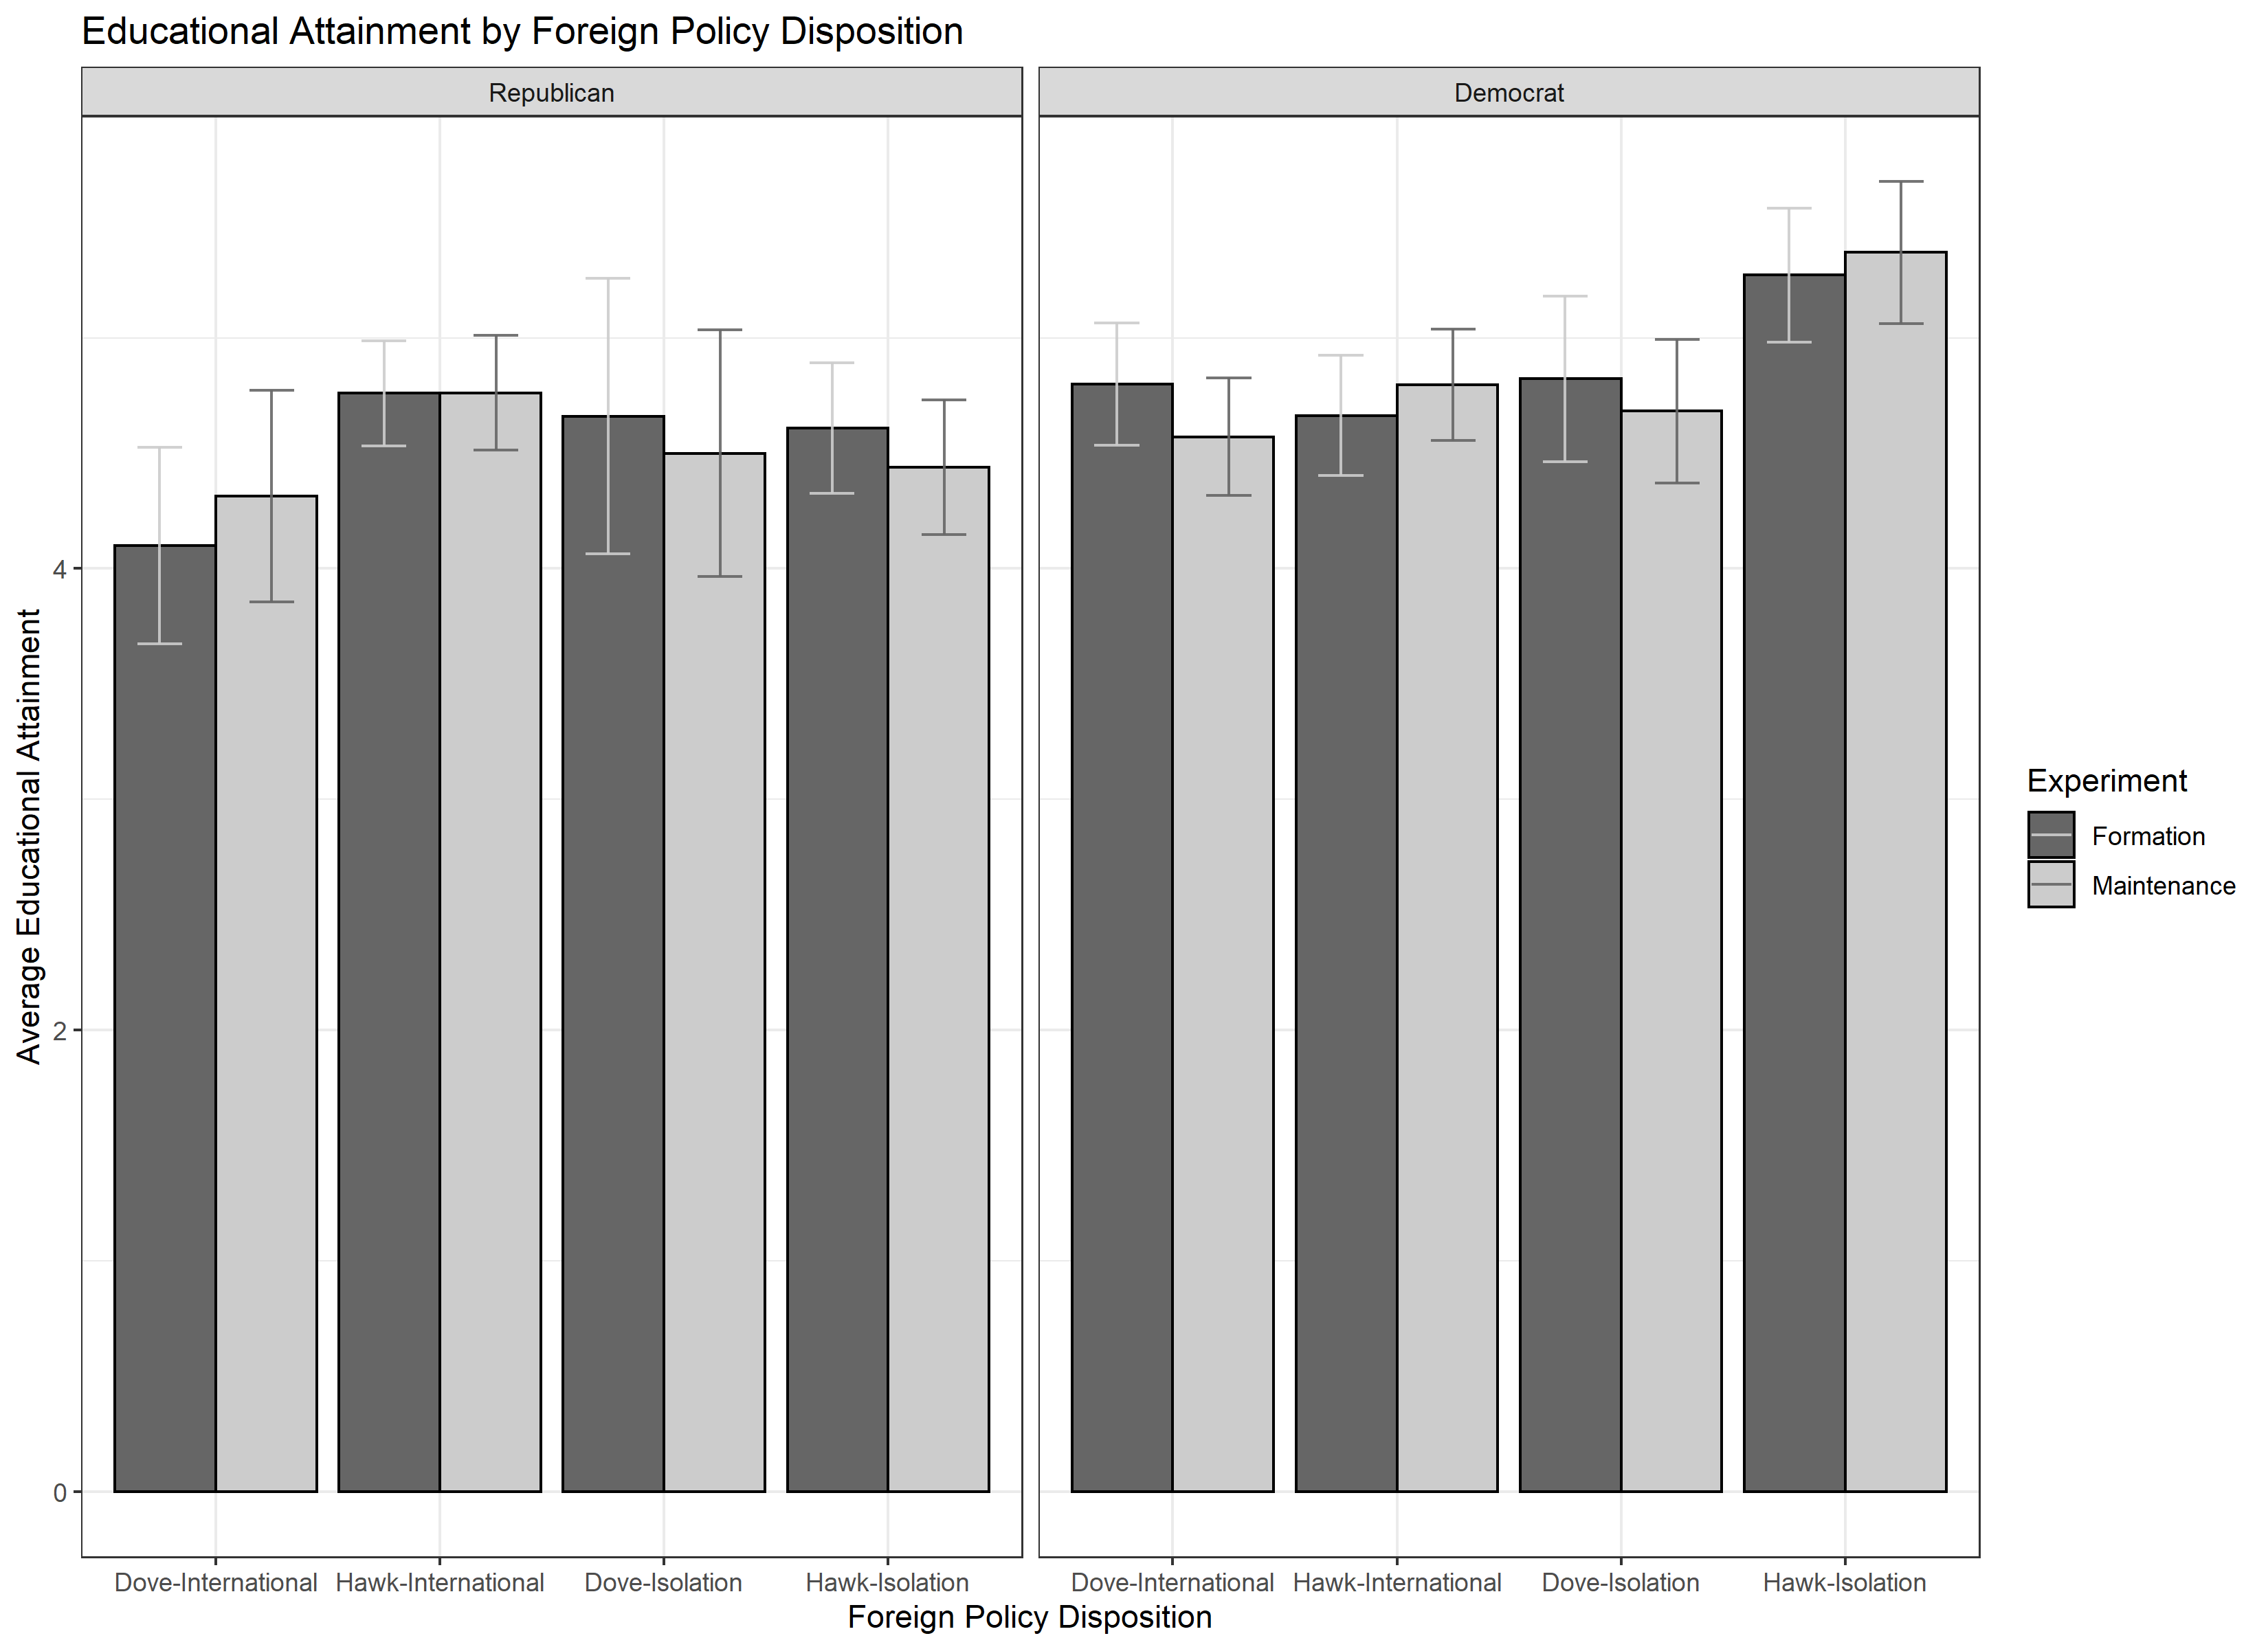
\includegraphics[width=0.95\textwidth]{part-educ-plots.png}
	\caption{Bar chart of partisan affiliation strength across foreign policy dispositions. Colors distinguish between the alliance formation and maintenance experiments. The error bars mark 95\% confidence interval of average partisan attachment.}
	\label{fig:part-educ-plots}
\end{figure}




\newpage




\section{Conjoint Treatment Frequency}

\autoref{fig:treat-freq} shows that the conjoint attributes appeared at similar rates in both experiments. 
 
\begin{figure}[htbp]
	\centering
		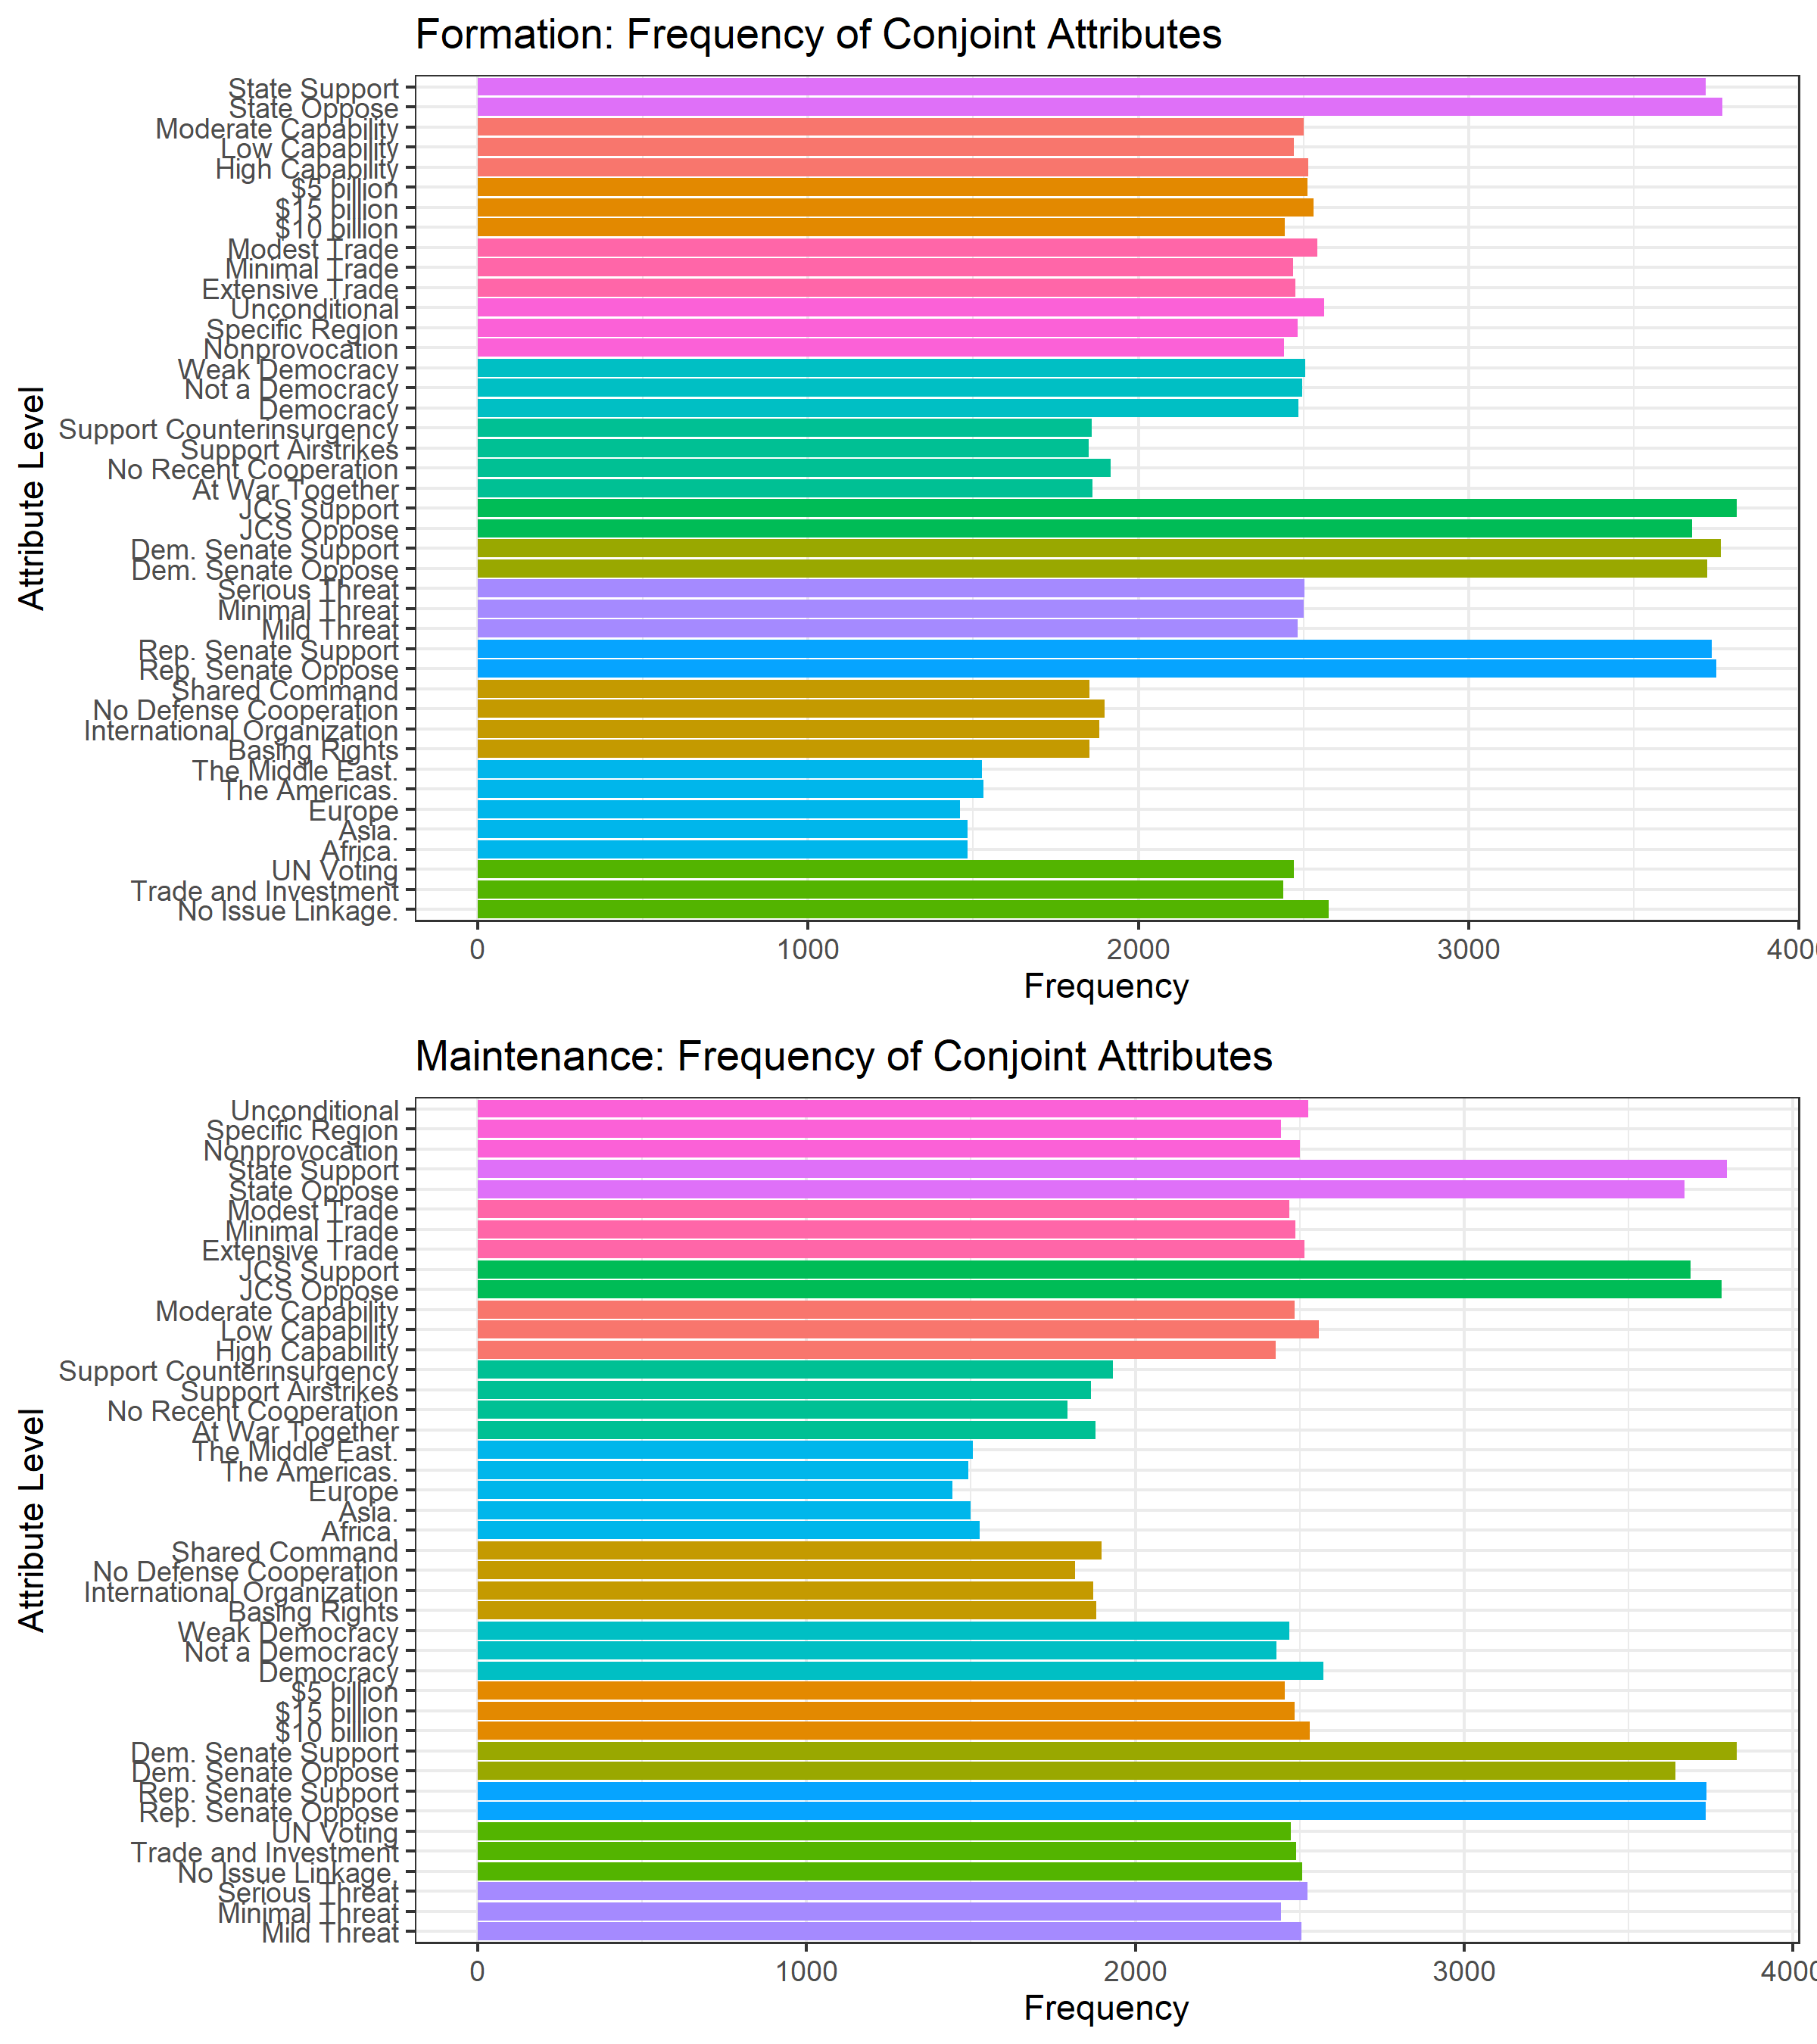
\includegraphics[width=0.95\textwidth]{treat-freq.png}
	\caption{Frequency of each conjoint experiment attribute in the alliance formation and maintenance conjoint experiments. Colors mark the attribute, while the y-axis values specify each level and the x-axis is the number of times an attribute level appeared in the conjoint alliance tables.}
	\label{fig:treat-freq}
\end{figure}


% Bibliography
\newpage 
 
\bibliography{../../MasterBibliography} 


\end{document}
